\documentclass[12pt,a4paper]{article}
\usepackage[top=2cm,bottom=2cm,left=3cm,right=2cm,includehead,includefoot,heightrounded]{geometry}
\usepackage[utf8]{vntex}
\usepackage{amsmath}
\usepackage{amsfonts}
\usepackage{amssymb}
\usepackage{caption}
\usepackage{graphicx}
\usepackage{fancyhdr}
\usepackage{fancybox}
\usepackage{lastpage}
\usepackage{listings}
\usepackage{courier}
\usepackage{indentfirst}
\usepackage{float}
\usepackage{enumitem}
\usepackage{longtable, tabularx}
\usepackage{color}
\usepackage[table,xcdraw]{xcolor}
\usepackage[normalem]{ulem}
\usepackage{multirow}
\usepackage{pdfpages}
\usepackage{times}
\usepackage{lscape}
\usepackage{titlesec}
\usepackage{rotating}
\usepackage{xurl}
\usepackage{etoolbox}
\usepackage{varwidth}
\usepackage{xcolor}
\usepackage[unicode]{hyperref}
\usepackage[flushmargin]{footmisc}

\addtolength{\footnotesep}{1mm}

\hypersetup{
  colorlinks,
  citecolor=blue,
  linkcolor=blue,
  urlcolor=blue}

\useunder{\uline}{\ul}{}

\setcounter{tocdepth}{3}
\setcounter{secnumdepth}{3}

\lstset{
tabsize = 4,
showstringspaces = false,
numbers = left,
commentstyle = \color{green},
keywordstyle = \color{blue},
stringstyle = \color{red},
rulecolor = \color{black},
basicstyle = \small \ttfamily,
breaklines = true,
numberstyle = \tiny,
}

\pagestyle{fancy}
\let\Sectionmark\sectionmark
\def\sectionmark#1{\def\Sectionname{#1}\Sectionmark{#1}}
\let\Subsectionmark\subsectionmark
\def\subsectionmark#1{\def\Subsectionname{#1}\Subsectionmark{#1}}
\let\Subsubsectionmark\subsubsectionmark
\def\subsubsectionmark#1{\def\Subsubsectionname{#1}\Subsubsectionmark{#1}}
\setlength{\headheight}{31pt}
\renewcommand{\headrulewidth}{2pt}
\renewcommand{\footrulewidth}{1pt}
\fancyhf{}
\fancyhead[L]{
  \begin{picture}(25,15)(0,0)
   \put(0,-8){
\includegraphics[width=9mm, height=9mm]{Img/Logo_BK.png}}
  \end{picture}
  \begin{tabular}{l}
    \textbf{Trường Đại học Bách Khoa - ĐHQG HCM}\\
    \textbf{Khoa Khoa học và Kỹ thuật Máy tính}
  \end{tabular}
}
\fancyhead[R]{
  \begin{tabular}{r}
    \textbf{LVTN - Survival2D}\\
    \textbf{\nouppercase{\leftmark}}
  \end{tabular}
}
\fancyfoot[C]{
  Trang {\thepage}/\pageref{LastPage}
}
\renewcommand\large{\fontsize{13pt}{13pt}\selectfont}
% \renewcommand{\sectionmark}[1]{\markboth{\MakeUppercase{\chaptername\ \thesection.\ #1}}{}}
\renewcommand{\sectionmark}[1]{\ifthenelse{\equal{0}{\thesection}}{\markboth{\MakeUppercase{#1}}{}}{\markboth{\MakeUppercase{\chaptername\ \thesection.\ #1}}{}}}
\newcommand{\todo}[1]{\textcolor{red}{\textit{//TODO: #1}}}
\begin{document}
  \newgeometry{top=2cm,bottom=2cm,left=3cm,right=2cm}
  \begin{titlepage}
    \thisfancypage{
      \doublebox}{}
    \begin{center}
    {\fontsize{15pt}{15pt}\selectfont
        ĐẠI HỌC QUỐC GIA THÀNH PHỐ HỒ CHÍ MINH\\
        TRƯỜNG ĐẠI HỌC BÁCH KHOA\\
        KHOA KHOA HỌC VÀ KỸ THUẬT MÁY TÍNH\\
        --------------------------o0o--------------------------
      }
    \end{center}
    \vspace{1cm}
    \begin{figure}[h!]
      \centering
      
\includegraphics[width=3cm]{Img/Logo_BK.png}
    \end{figure}
    \vspace{1cm}
    \begin{center}
      \textbf{\fontsize{16pt}{16pt}\selectfont BÁO CÁO\\}
      \textbf{\fontsize{16pt}{16pt}\selectfont LUẬN VĂN TỐT NGHIỆP ĐẠI HỌC\\}
      \vspace{1cm}
      \textbf{\fontsize{25pt}{25pt}\selectfont GAME SURVIVAL2D\\}
      \vspace{1cm}
      \fontsize{15pt}{15pt}\selectfont Ngành: Khoa học Máy tính\\
    \end{center}
    \vspace{1cm}
    \begin{table}[h]
      \centering
      \fontsize{15pt}{15pt}\selectfont
      \begin{tabular}{rrll}
        & \textbf{Hội đồng}: & \textbf{Khoa học Máy tính} & \\
        & \textbf{GVHD}: & \textbf{ThS. Vương Bá Thịnh} & \\
        & \textbf{GVPB}: & \textbf{KS. Trần Huy} & \\
        \multicolumn{4}{c}{\textbf{---o0o---}} \\
        & \textbf{SVTH 1:} & \textbf{Trần Minh Quân} & \textbf{(1712831)} \\
        & \textbf{SVTH 2:} & \textbf{Nguyễn Minh Tiến} & \textbf{(1713484)} \\
      \end{tabular}
    \end{table}
    \vspace{3cm}
    \begin{center}
      {\fontsize{15pt}{15pt}\selectfont TP. Hồ Chí Minh, Tháng 05/2023}
    \end{center}
  \end{titlepage}
  \restoregeometry

  % 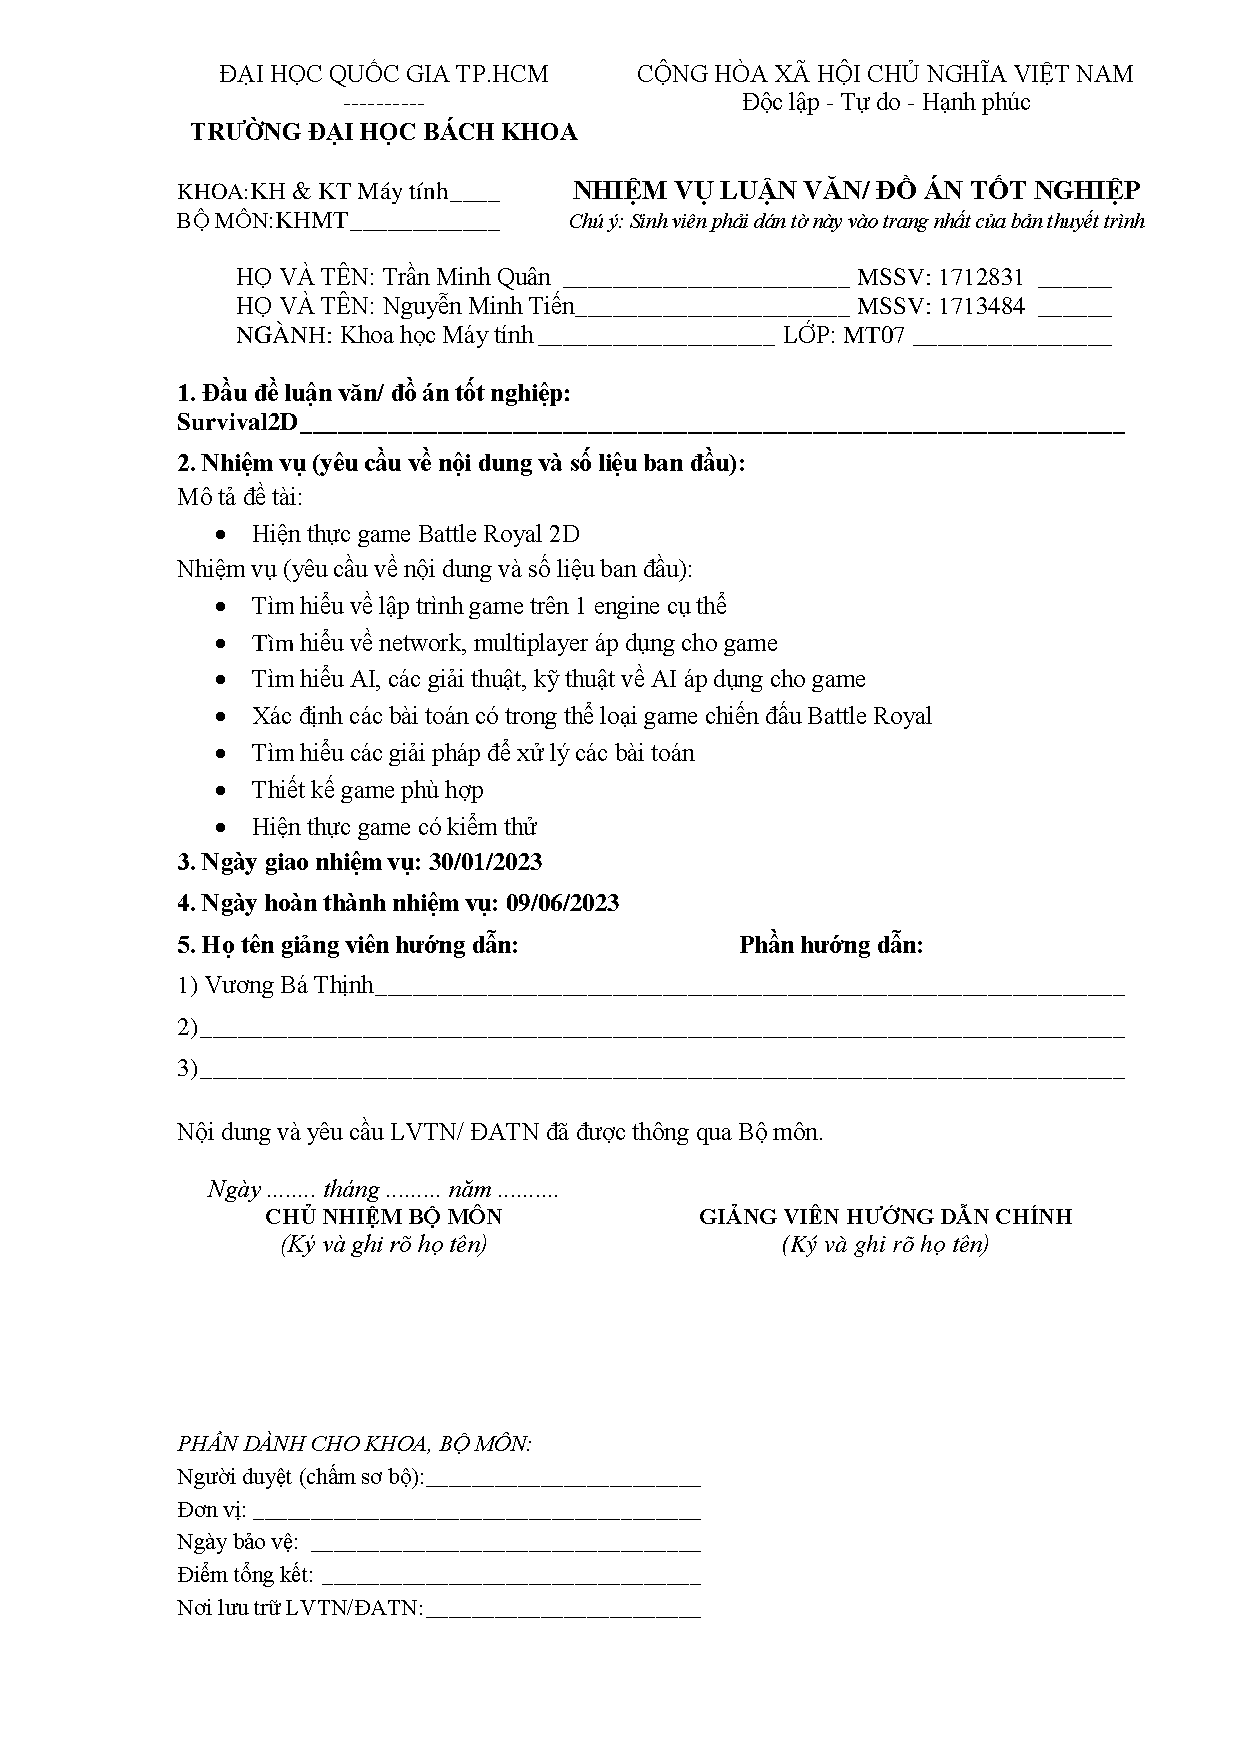
\includepdf[pages=-]{phieunhiemvu.pdf}
  
  \newpage
  \section*{\centering LỜI CAM ĐOAN}\sectionmark{Lời cam đoan}
  Nhóm xin cam đoan đề tài này là thành quả nghiên cứu của riêng mình, dưới sự hướng dẫn của ThS. Vương Bá Thịnh. Các nội dung nghiên cứu, phân tích và kết quả trong đề tài này là trung thực và chưa công bố dưới bất kỳ hình thức nào trước đây.

  Nếu phát hiện có bất kỳ sự gian lận nào, nhóm hoàn toàn chịu trách nhiệm về nội dung đề tài luận văn của mình và chịu mọi hình thức kỷ luật trước Ban chủ nhiệm Khoa và Ban giám hiệu nhà trường.

  \newpage
  \section*{\centering LỜI CẢM ƠN}\sectionmark{Lời cảm ơn}
  Trước hết, nhóm xin cảm ơn thầy Vương Bá Thịnh đã đồng hành cùng nhóm trong suốt thời gian thực hiện đề tài. Cảm ơn thầy Trần Huy vì những góp ý quý giá của thầy trong buổi phản biện đề tài, đã giúp nhóm nhận ra nhiều thiếu sót trước đó và chỉnh sửa lại hoàn thiện hơn. Cảm ơn các thầy, cô trong khoa Khoa học và Kỹ thuật Máy tính, trường Đại học Bách Khoa, Đại học Quốc gia Thành phố Hồ Chí Minh đã truyền đạt kiến thức trong những năm học tập. Những tri thức quý báu ấy đã giúp nhóm có thể vận dụng để làm nên đề tài này.
  
  Nhóm cũng xin cảm ơn các sếp, các bạn đồng nghiệp tại ZingPlay Game Studios, quá trình làm việc ở đây đã giúp các thành viên trong nhóm trau dồi kinh nghiệm thực tế trong quá trình làm ra một game. Các bạn cũng là những người tạo nguồn cảm hứng cho việc lựa chọn một chủ đề về game làm đề tài luận văn tốt nghiệp.

  Vì khả năng của bản thân còn hạn chế, trong quá trình làm đề tài nhóm không tránh khỏi những sai sót, kính mong nhận được ý kiến đóng góp từ thầy cô và các bạn để đề tài được hoàn thiện hơn.

  Cuối cùng, nhóm xin chân thành cảm ơn thầy cô và các bạn đã dành thời gian đọc tài liệu này.
  
  \newpage
  \section*{\centering TÓM TẮT ĐỀ TÀI}\sectionmark{Tóm tắt đề tài}
  \textbf{Survival2D} là game bắn súng Battle Royale lấy ý tưởng từ game Player Unknown Battle Ground (PUBG). \textbf{Survival2D} sử dụng đồ hoạ 2D, không yêu cầu phần cứng cao; thích hợp chơi trên trình duyệt web, điện thoại, có thể tiếp cận với các nền tảng không thường được sử dụng để chơi game nhiều như Linux và MacOS.
  
  Báo cáo này gồm 9 chương, bao gồm: giới thiệu đề tài, thiết kế game, công nghệ sử dụng, phân tích hệ thống, thiết kế hệ thống, kiểm thử, đánh giá kết quả đạt được, định hướng phát triển và công cụ sử dụng.
  
  Chương giới thiệu đề tài trình bày tổng quan về nội dung, mục tiêu và giới hạn của đề tài.

  Chương thiết kế game trình bày về luật game và các phần liên quan đến thiết kế của game.
  
  Chương công nghệ sử dụng trình bày các công nghệ đã được sử dụng khi triển khai hệ thống.
  
  Chương phân tích hệ thống trình bày các vấn đề lớn gặp phải để hiện thực được game.
  
  Chương thiết kế hệ thống trình bày định hướng giải quyết các vấn đề lớn kể trên.

  Chương kiểm thử trình bày các kết quả kiểm thử sau khi hiện thực đề tài.

  Chương đánh giá kết quả đạt được trình bày các kết quả mà nhóm đã đạt được sau quá trình thực hiện luận văn, và đánh giá kết quả này.
  
  Chương định hướng phát triển trình bày ưu điểm, nhược điểm và hướng phát triển của đề tài.

  Chương công cụ sử dụng liệt kê các công cụ mà nhóm đã sử dụng trong quá trình thực hiện đề tài, tạo thành sản phẩm.
  
  \newpage
  % \renewcommand\contentsname{Mục lục}
  % \addcontentsline{toc}{section}{Mục lục}
  \tableofcontents
  
  \newpage
  \renewcommand\listfigurename{Danh sách hình ảnh}
  % \addcontentsline{toc}{section}{Danh sách hình ảnh}
  \listoffigures
  
  \newpage
  % \renewcommand\listtablename{Danh sách bảng}
  % \addcontentsline{toc}{section}{Danh sách bảng}
  \listoftables
  
  \newpage
  \section{Giới thiệu đề tài}
  \subsection{Sơ lược về thể loại game Battle Royale}

  Battle Royale là thể loại game bắn súng sinh tồn nhiều người chơi (multiplayer), với yếu tố sống còn được đặt lên hàng đầu. Trong mỗi trận đấu, người chơi phải thu thập vũ khí, trang bị để trở nên mạnh hơn, khi thời gian trôi qua thì khu vực an toàn sẽ thu hẹp lại buộc các người chơi phải chiến đấu với nhau, và người sống sót cuối cùng là người chiến thắng. Bên cạnh tính hành động, chiến thuật, Battle Royale còn đòi hỏi người chơi tinh thần đồng đội khi chơi theo nhóm, hỗ trợ lẫn nhau để giành chiến thắng cuối cùng.

  \subsection{Vấn đề của thể loại game Battle Royale}
  Trên thị trường hiện tại đã có một số tựa game Battle Royale nổi tiếng và thành công như PUBG, CS:GO, Valorant, PUBG Mobile, Free Fire,... nhưng tất cả đều có những nhược điểm nhất định. Những tựa game kể trên đều có đồ hoạ 3D, yêu cầu cấu hình máy trung bình đến cao, khó tiếp cận những người dùng phổ thông. Một vài game khi đã có được lượng người chơi khủng thì lại không giữ được lâu.
  
  Lấy ví dụ với PUBG, tựa game đã từng rất hot ở thời điểm năm 2018 với hơn 3 triệu người chơi nhưng hiện nay chỉ còn khoảng 1/10 con số này:
  \begin{figure}[H]
      \centering
      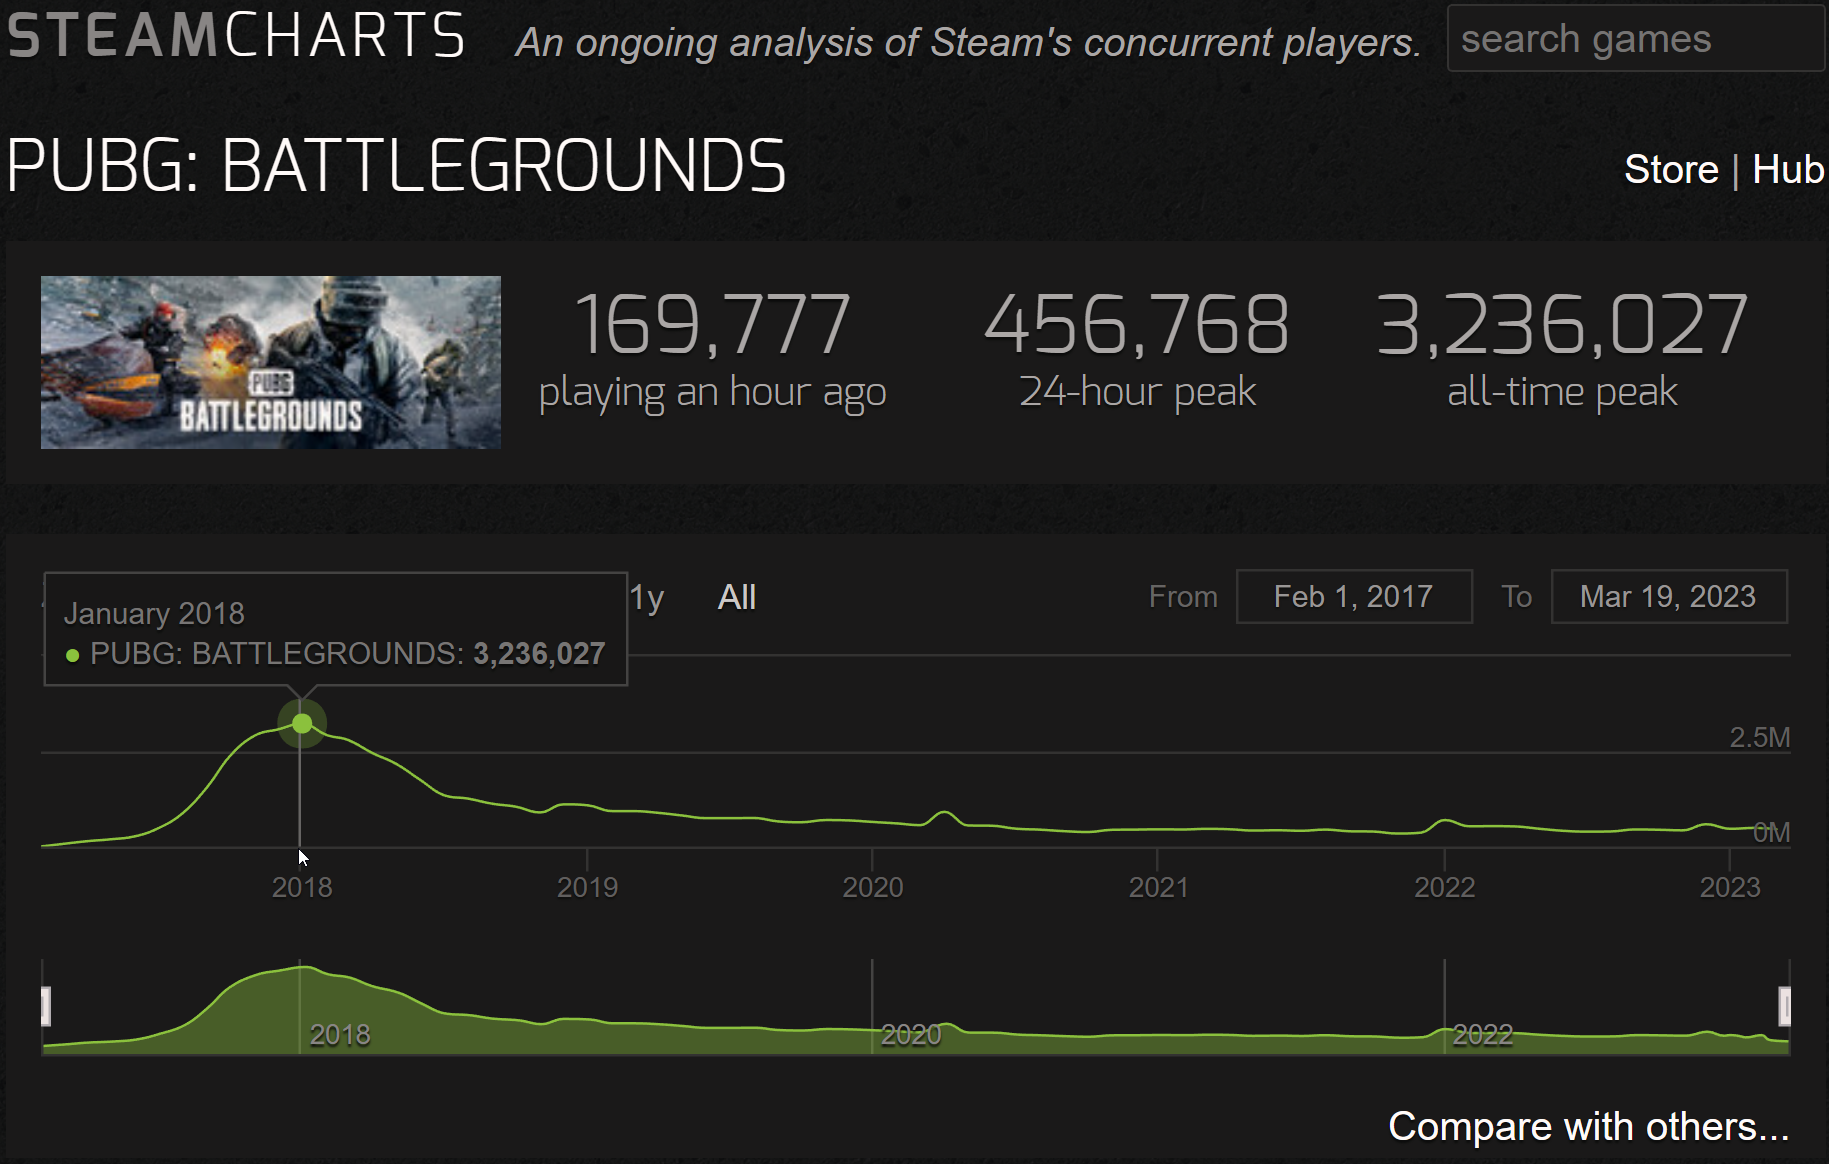
\includegraphics[width=\textwidth]{Img/intro/PUBG.png}
      \caption[Biểu đồ PUBG]{Biểu đồ lượng người chơi của PUBG{\protect\footnotemark}}
  \end{figure}
  \footnotetext{Nguồn: \url{https://steamcharts.com/app/578080##All}}
  
  Hai trong số nhiều lý do dẫn đến việc PUBG đi xuống đó là nạn hack cheat và gameplay nhàm chán không có nhiều thay đổi đáng kể từ lúc phát hành.\footnotemark
  Nạn hack/cheat\footnotemark là điều khá thường thấy ở các tựa game online nói chung và game bắn súng Battle Royale nói riêng. Nhiều tựa game đã "chết" vì lý do chính là nạn hack quá nhiều. Nạn hack vừa làm mất cân bằng game, gây bất lợi cho người chơi không dùng hack, vừa làm mất uy tín của nhà phát hành.
  
  Một trong những thể loại hack phổ biến của dòng game Battle Royale là cheat ESP. Đây là tình trạng người chơi có thể sử dụng công cụ bên ngoài, truy cập trái phép vào dữ liệu của game; để có thể nhìn xuyên địa hình, vật thể, thấy được người chơi khác nhằm chiếm lợi thế trong game.
  
  \footnotetext{PUBG và những lý do trở thành dead game: \url{https://www.youtube.com/watch?v=i6KC0xFBn5U}}

  \subsection{Mục tiêu của Survival2D}

  Nhận ra thiếu sót của các tựa game Battle Royale hiện có, nhóm mong muốn tạo ra một tựa game mới, thể loại chiến đấu sinh tồn, tên là \textbf{Survival2D}. \textbf{Survival2D} sẽ khắc phục những điểm chưa tốt của những tựa game đi trước, giải quyết được các vấn đề của dòng game Battle Royale, với các đặc điểm sau:
  
  \begin{itemize}
      \item \textit{Thể loại Battle Royale multiplayer, đồ hoạ 2D}: Game nhiều người chơi cùng lúc, đồ hoạ đơn giản, không yêu cầu cấu hình cao, có thể chơi trên đa nền tảng, dễ tiếp cận với nhiều người chơi ở các tập người chơi khác nhau.
      \item \textit{Hạn chế hack/cheat ESP}: Như đã nói ở trên, các dòng game Battle Royale thường có hạn chế là bị hack ESP. \textbf{Survival2D} sẽ phát triển cơ chế bảo mật để không thể hack cheat ESP, mang lại trải nghiệm tốt hơn cho người chơi.
      \item \textit{Có người chơi máy}: Có người chơi máy để đấu với người chơi khi số lượng người chơi online thấp, dẫn đến không thể ghép trận với các người chơi khác. Bot đảm bảo có thể thực hiện các hành động một player thông thường có thể làm: di chuyển, nhặt vũ khí, vật phẩm, chiến đấu,... và có thể cạnh tranh chiến thắng với người chơi thật.
  \end{itemize}
  \footnotetext{Những phương thức để giết chết một game online (GameK): \url{https://gamek.vn/game-online/nhung-phuong-thuc-de-giet-chet-mot-game-online-20130531061110655.chn}}
  
  \subsection{Giới hạn}
  
  Trong quá trình phát triển \textbf{Survival2D}, nhóm nhận thấy một số chức năng hay, có thể đưa vào mở rộng game để tăng trải nghiệm người chơi nhưng vì giới hạn về nhân lực và thời gian, nhóm chưa hoàn thành được trong đề tài này, như là: chơi theo nhóm, cho âm thanh vào game, phương tiện di chuyển, cho phép người chơi tương tác nhiều hơn với đồng đội (tin nhắn, thoại,...). Thay vào đó, nhóm sẽ ưu tiên phát triển đầy đủ các tính năng cơ bản của một game chiến đấu, và sau đó tập trung vào những vấn đề chính để hoàn thành mục tiêu của đề tài, bao gồm:

  \begin{itemize}
      \item Hiện thực game đồ hoạ 2D trên nền tảng web (và có khả năng mở rộng lên đa nền tảng), thoả mãn yêu cầu:
        \begin{itemize}
            \item Gameplay đầy đủ tính năng của một game Battle Royale
            \item Đáp ứng được 5-10 người chơi cùng lúc
            \item Đồng bộ dữ liệu giữa các client giống nhau theo thời gian thực
            \item Ping trung bình dưới 50ms trong điều kiện mạng phổ thông ở Việt Nam
        \end{itemize}
      \item Hiện thực phương pháp giải quyết nạn cheat ESP
      \item Hiện thực người chơi máy áp dụng các giải thuật AI, có đầy đủ các hành vi chơi game giống với người chơi thật.
  \end{itemize}

\newpage
\section{Thiết kế game}
  Dưới đây là các thiết kế của game \textbf{Survival2D}:
  \subsection{Luật game}
  Trò chơi sinh tồn: người chơi lập nhóm gồm 1 hoặc nhiều người, sau đó được đưa vào một bản đồ, chiến đấu với nhau đến khi chỉ còn 1 người hoặc 1 nhóm cuối cùng.
  
  Khi vào một trận đấu, người chơi sẽ xuất hiện ngẫu nhiên trên map, nếu là nhóm thì vị trí các thành viên sẽ gần nhau. Sau đó người chơi tìm nhặt vũ khí, vật phẩm trên map, chiến đấu với nhau để sinh tồn cho đến khi chỉ còn 1 người hoặc 1 nhóm; nhóm cuối cùng này sẽ là nhóm chiến thắng.
  
  Người chơi có một lượng máu nhất định, máu sẽ giảm khi người chơi bị bắn trúng. Có thể dùng vật phẩm hồi máu để tăng máu trở lại. Nếu chơi đơn thì hết máu sẽ chết, nếu chơi nhóm thì hết máu sẽ bị vào trạng thái "knock", trạng thái này người chơi sẽ có "thanh máu knock", thanh máu này giảm dần theo thời gian, hết thanh máu knock sẽ chết hẳn. Trong trạng thái knock, đồng đội có thể cứu, sau đó người chơi sẽ trở lại trạng thái bình thường với rất ít máu.

  \subsection{Bản đồ}
  Bản đồ hình chữ nhật, trên bản đồ rải rác các vật cản, vật phẩm. Các vật cản, vật phẩm trên bản đồ và vị trí ban đầu của người chơi được sắp xếp để đảm bảo cân bằng giữa các người chơi.

  \subsection{Vùng an toàn (Safe zone)}\label{safezone}\mbox{}

  \begin{figure}[H]
      \centering
      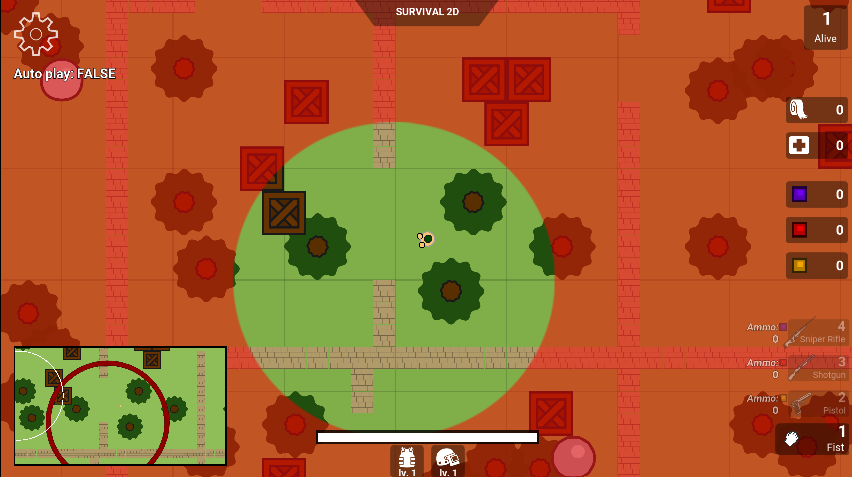
\includegraphics[width=1\textwidth]{Img/game_screen_shoot/safe_zone.png}
      \caption{Vùng an toàn (Safe zone) trong \textbf{Survival2D}}
  \end{figure}
  
  Lấy ý tưởng từ PUBG, \textbf{Survival2D} cũng có một vùng bao quanh được gọi là vùng an toàn (safe zone), còn có tên khác là \textit{bo}. Người chơi ở ngoài vòng \textit{bo} này sẽ bị mất máu mỗi giây. Đây là biện pháp để sau khi người chơi đã tiêu diệt bớt đối thủ thì sẽ nhanh chóng tìm được đối thủ khác (do đứng bên ngoài \textit{bo} sẽ bị bất lợi mất máu, người chơi sẽ cố gắng tập trung lại bên trong vòng \textit{bo} này để được lợi thế), và cũng hạn chế người chơi thích ẩn nấp, rình rập, tránh chiến đấu để sinh tồn. \textit{Bo} sẽ thu hẹp lại sau một thời gian, và đến một lúc sẽ không còn nữa, đồng nghĩa tất cả người chơi đều sẽ bị mất máu đến khi trò chơi kết thúc.

  \subsection{Vật cản}
  \begin{figure}[H]
      \centering
      
\includegraphics[width=0.2\textwidth]{Img/game_screen_shoot/tree.png}
      
\includegraphics[width=0.2\textwidth]{Img/game_screen_shoot/stone_1.png}
      
\includegraphics[width=0.2\textwidth]{Img/game_screen_shoot/crate.png}
      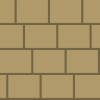
\includegraphics[width=0.2\textwidth]{Img/game_screen_shoot/wall.png}
      \caption{Vật cản trong \textbf{Survival2D}: cây, đá, thùng, tường}
  \end{figure}
  \textbf{Survival2D} có các loại vật cản sau:
\begin{table}[H]
\centering
\begin{tabular}{|l|l|l|l|}
\hline
\multicolumn{1}{|c|}{\textbf{Vật cản}} & \multicolumn{1}{c|}{\textbf{Hình dạng}} & \multicolumn{1}{c|}{\textbf{Kích thước}} & \multicolumn{1}{c|}{\textbf{Đặc tính}} \\ \hline
Cây & Tròn & \begin{tabular}[c]{@{}l@{}}Thân cây: 50x50\\ Tán lá: 150x150\end{tabular} & \begin{tabular}[c]{@{}l@{}}Có thể bị phá huỷ\\ Bao gồm thân cây và tán lá\\ Có thể nấp dưới tán lá\end{tabular} \\ \hline
Thùng & Vuông & 200x200 & \begin{tabular}[c]{@{}l@{}}Có thể bị phá huỷ\\ Khi bị phá huỷ rơi ra vật phẩm\end{tabular} \\ \hline
Đá & Tròn & 100x100 & \begin{tabular}[c]{@{}l@{}}Có thể bị phá huỷ\\ Chủ yếu để tránh né đạn của địch\end{tabular} \\ \hline
Tường & Vuông & 100x100 & \begin{tabular}[c]{@{}l@{}}Không thể bị phá huỷ\\ Liên kết với nhau để phân chia bản đồ\\ Tạo hình dạng giống mê cung\end{tabular} \\ \hline
\end{tabular}
\caption{Chi tiết các loại vật cản trong \textbf{Survival2D}}
\end{table}

  \subsection{Người chơi}
  \begin{figure}[H]
      \centering
      
\includegraphics[width=0.5\textwidth]{Img/game_screen_shoot/player.png}
      \caption{Người chơi trong \textbf{Survival2D}: tay không và cầm súng}
  \end{figure}
  Khi vừa vào trận đấu, người chơi sẽ có sẵn 100 máu. Người chơi được biểu diễn là 2 hình tròn đồng tâm gồm hình tròn ngoài bán kính 30 thể hiện \textit{cơ thể}, hình tròn trong bán kính 10 thể hiện \textit{đầu}, cùng với 2 hình tròn nhỏ ở phía trước thể hiện 2 \textit{tay}. Khi \textit{cơ thể} bị đấm trúng hoặc bị đạn xuyên qua, người chơi sẽ nhận sát thương và mất máu. Sát thương trúng vào \textit{đầu} sẽ tăng lên nhiều lần so với trúng vào \textit{cơ thể}.

  \subsection{Vũ khí}
  \textbf{Survival2D} có các loại vũ khí sau:
\begin{table}[H]
\centering
\begin{tabular}{|l|c|c|c|c|l|}
\hline
\multicolumn{1}{|c|}{\textbf{Vũ khí}} & \textbf{\begin{tabular}[c]{@{}c@{}}Tầm\\ bắn\end{tabular}} & \textbf{\begin{tabular}[c]{@{}c@{}}Sát thương\\ lên cơ thể\end{tabular}} & \textbf{\begin{tabular}[c]{@{}c@{}}Sát thương\\ lên đầu\end{tabular}} & \textbf{\begin{tabular}[c]{@{}c@{}}Sức\\ chứa\end{tabular}} & \multicolumn{1}{c|}{\textbf{Đặc điểm}}                                                          \\ \hline
Tay không                             & 10                                                         & 5                                                                        & 15                                                                    &                                                             & \begin{tabular}[c]{@{}l@{}}Không cần đạn để tấn công\\ Không cần thay đạn\end{tabular}          \\ \hline
Súng ngắn                             & 500                                                        & 10                                                                       & 30                                                                    & 20                                                          & \begin{tabular}[c]{@{}l@{}}Lượng đạn súng ngắn\\ trên bản đồ nhiều\end{tabular}                 \\ \hline
Súng săn                              & 500                                                        & 20                                                                       & 60                                                                    & 5                                                           & \begin{tabular}[c]{@{}l@{}}Khi bắn tạo ra 5 luồng đạn\\với độ lệch không xác định\end{tabular} \\ \hline
Súng bắn tỉa                          & 1500                                                       & 30                                                                       & 90                                                                    & 10                                                          & Tầm bắn xa, sát thương lớn                                                                      \\ \hline
\end{tabular}
\caption{Thông số các loại vũ khí trong \textbf{Survival2D}}
\end{table}

   \begin{figure}[H]
      \centering
      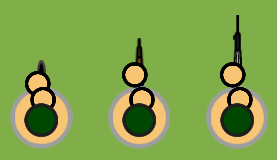
\includegraphics[width=0.5\textwidth]{Img/game_screen_shoot/player_gun.png}
      \caption{Các loại súng trong \textbf{Survival2D}. Từ trái qua: súng ngắn, súng săn và súng bắn tỉa}
  \end{figure}

  \subsection{Trang bị}
  \textbf{Survival2D} có các loại trang bị sau:
\begin{table}[H]
\centering
\begin{tabular}{|l|l|}
\hline
\multicolumn{1}{|c|}{\textbf{Trang bị}} & \multicolumn{1}{c|}{\textbf{Tác dụng}} \\ \hline
Nón & Giảm 30\% sát thương vào đầu \\ \hline
Giáp & Giảm 30\% sát thương lên cơ thể \\ \hline
\end{tabular}
\caption{Chỉ số các loại trang bị trong \textbf{Survival2D}}
\end{table}
  \begin{figure}[H]
      \centering
      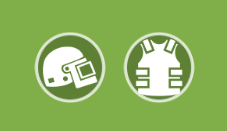
\includegraphics[width=0.5\textwidth]{Img/game_screen_shoot/trang_bi.png}
      \caption{Nón và giáp trong \textbf{Survival2D}}
  \end{figure}
  
  \subsection{Vật phẩm}
  \textbf{Survival2D} có các loại vật phẩm sau:
\begin{table}[H]
\centering
\begin{tabular}{|l|l|}
\hline
\multicolumn{1}{|c|}{\textbf{Vật phẩm}} & \multicolumn{1}{c|}{\textbf{Tác dụng}} \\ \hline
Bộ sơ cứu & Hồi 80\% máu đã mất \\ \hline
Băng cứu thương & Hồi 20\% máu đã mất \\ \hline
\end{tabular}
\caption{Chỉ số các loại vật phẩm trong \textbf{Survival2D}}
\end{table}
  \begin{figure}[H]
      \centering
      
\includegraphics[width=0.5\textwidth]{Img/game_screen_shoot/items.png}
      \caption{Bộ sơ cứu và băng cứu thương trong \textbf{Survival2D}}
  \end{figure}
  
  \newpage
  \section{Công nghệ sử dụng}
  \subsection{Client}
  \subsubsection{Cocos2d-x}
  \textbf{Survival2D} là game trực tuyến nhiều người chơi, và hướng đến nền tảng trình duyệt; vì vậy client của \textbf{Survival2D} yêu cầu một game engine phải gọn nhẹ và có khả năng hỗ trợ đa nền tảng. Cocos2d-x là một engine phát triển game nổi tiếng, ra mắt từ lâu nhưng vẫn đang được sử dụng phổ biến hiện nay, đáp ứng được những yêu cầu trên.
  
  \paragraph{Ưu điểm}
  \begin{itemize}
      \item Miễn phí và có mã nguồn mở.
      \item Gọn nhẹ, dễ dàng cài đặt và sử dụng, có thể chạy mượt mà trên các máy tính với cấu hình không cần quá cao.
      \item Hỗ trợ nhiều ngôn ngữ lập trình khác nhau, trong đó có C++ để tối ưu hiệu năng, hay JavaScript để lập trình nhanh chóng, dễ dàng.
      \item Hỗ trợ phát triển chủ yếu game đồ hoạ 2D, Cocos2d-x vẫn là một engine mạnh mẽ, tốc độ phát triển và dựng game nhanh.
      \item Hỗ trợ đa nền tảng, đáp ứng mục tiêu của game là tiếp cận được nhiều người chơi, bên cạnh đó cũng mang lại tiện lợi trong quá trình phát triển game, giúp nhóm dễ dàng test game mà không sợ thiếu thiết bị.
  \end{itemize}

  \paragraph{Nhược điểm}
  \begin{itemize}
      \item Engine đã cũ, không có nhiều tiện ích như các engine khác.
      \item Tài liệu khó tìm, ít nhận được sự hỗ trợ từ cộng đồng.
      \item Còn tồn tại một số lỗi nhưng đã không còn được bảo trì, không được nâng cấp và vá lỗi.
  \end{itemize}

  Tuy có vài nhược điểm như đã nêu trên nhưng các nhược điểm này không quá lớn; bên cạnh đó những ưu điểm của Cocos2d-x là rất phù hợp với mục tiêu của đề tài: game 2D, gọn nhẹ, dễ tiếp cận nhiều tập người chơi.
  
  \paragraph{Một số engine khác để so sánh}
  \subparagraph{Unity}
  \begin{itemize}
      \item Ưu điểm:
      \begin{itemize}
          \item Miễn phí.
          \item Phổ biến, có sẵn nhiều tài liệu để học và cộng đồng đông đảo dễ tìm kiếm sự hỗ trợ, có nhiều asset và plugin.
          \item Hỗ trợ đa nền tảng.
          \item Cung cấp nhiều tính năng có sẵn: editor mạnh mẽ, trực quan, hỗ trợ xây dựng scene,... hỗ trợ yếu tố vật lý, âm thanh,...
      \end{itemize}
      \item Nhược điểm:
      \begin{itemize}
          \item Mã nguồn đóng.
          \item Có quá nhiều thành phần khiến người mới tiếp cận bị choáng ngợp.
          \item Hỗ trợ game 3D nên khá nặng, cần máy tính đủ mạnh để sử dụng, không cần thiết đối với quy mô của đề tài.
          \item Khó kiểm thử do không mở được 2 instance game cùng lúc trong khi đang phát triển.
      \end{itemize}
  \end{itemize}
  \subparagraph{Unreal Engine}
  \begin{itemize}
      \item Ưu điểm:
      \begin{itemize}
          \item Miễn phí
          \item Hiệu năng tuyệt vời, do tận dụng sự tối ưu của C++
          \item Mã nguồn có thể truy cập được
      \end{itemize}
      \item Nhược điểm:
      \begin{itemize}
          \item Chỉ hỗ trợ C++, khó dùng.
          \item Khá nặng, chú trọng đồ hoạ 3D (thích hợp cho game AAA hơn), không cần thiết đối với quy mô và mục tiêu của \textbf{Survival2D}.
          \item Asset store chưa bằng Unity.
      \end{itemize}
  \end{itemize}
  \subparagraph{Cocos Creator}
  \begin{itemize}
      \item Ưu điểm:
      \begin{itemize}
          \item Là phiên bản engine thế hệ mới của Cocos2d-x.
          \item Khắc phục lỗi từ Cocos2d-x, cung cấp thêm những tính năng mới, có editor mạnh, trực quan như Unity.
          \item Có tài liệu tham khảo tốt hơn, cộng đồng phát triển hơn.
      \end{itemize}
      \item Nhược điểm:
      \begin{itemize}
          \item Tuy mới nhưng chưa hoàn thiện, vẫn còn khó sử dụng, khó tích hợp với các library của NodeJS để mở rộng, chưa đạt được hiệu quả cao.
          \item Tương tự Unity, Cocos Creator đã chú trọng hơn về game 3D, không cần thiết đối với quy mô của đề tài.
      \end{itemize}
  \end{itemize}

  Tổng hợp lại từ ưu nhược điểm của các engine phổ biến kể trên, bảng so sánh dưới đây thể hiện mức độ hiệu quả, đáp ứng yêu cầu về 3 tiêu chí khi chọn một engine để phát triển \textbf{Survival2D} cơ bản như sau:

\begin{table}[H]
\centering
\begin{tabular}{|l|l|l|l|l|}
\hline
                                                                               & Cocos2d-x & Unity & Unreal Engine & Cocos Creator \\ \hline
\begin{tabular}[c]{@{}l@{}}Hỗ trợ phát triển tốt\\ game đồ hoạ 2D\end{tabular} & Có        & Có    & Có            & Có            \\ \hline
Engine gọn nhẹ                                                                 & Có        & Không & Không         & Không         \\ \hline
Dễ sử dụng                                                                     & Có        & Có    & Không         & Có            \\ \hline
\end{tabular}
\caption{So sánh mức độ đáp ứng yêu cầu giữa các game engine}
\end{table}

  Đa số các engine tuy mạnh và nhiều tiện ích nhưng đều hướng đến phát triển game 3D, game cấu hình cao, rất dư thừa vì \textbf{Survival2D} không dùng đến những tiện ích đó, hơn nữa các phần không cần thiết này có thể ảnh hưởng đến hiệu năng của \textbf{Survival2D}. Vì vậy Cocos2d-x là sự lựa chọn vừa đủ và phù hợp nhất để nhóm phát triển client của \textbf{Survival2D}.
  
  \subsection{Server}
  \subsubsection{Java}
  \paragraph{Tổng quan}\mbox{}\\
  Là một game nhiều người chơi, server của \textbf{Survival2D} cần hỗ trợ nhiều người chơi cùng lúc, xử lý nhiều trận đấu cùng lúc, đồng thời có thể tối ưu hoá bộ nhớ bởi vì lượng object trong một trận đấu là cực kỳ nhiều. Nhóm lựa chọn Java vì Java có thể thoả mãn những yêu cầu trên.

  \paragraph{Ưu điểm}
  \begin{itemize}
    \item Ngôn ngữ bậc cao: Java là ngôn ngữ bậc cao, hướng đối tượng dễ tiếp cận.
    \item Đa nền tảng: Java có thể chạy trên nhiều kiến trúc máy tính và hệ điều hành khác nhau.
    \item Bảo mật cao: Java có tính bảo mật cao, bao gồm kiểm soát quyền truy cập, phát hiện và ngăn chặn các lỗ hổng bảo mật, và mã hóa dữ liệu để bảo vệ thông tin của người dùng.
    \item Xử lý đa luồng hiệu quả: Java hỗ trợ xử lý đa luồng, giúp tăng hiệu suất và độ tin cậy của các ứng dụng phát triển trên nền tảng Java.
    \item Quản lý bộ nhớ tự động: Java có bộ thu gom rác tự động, giúp quản lý bộ nhớ và giải phóng bộ nhớ không còn sử dụng nữa.
    \item Độ tin cậy cao: Java có tính năng kiểm tra kiểu dữ liệu trực tiếp trong quá trình biên dịch, giúp giảm thiểu khả năng xảy ra lỗi liên quan đến kiểu dữ liệu.
    \item Kho thư viện phong phú: Java có kho thư viện của bên thứ 3 rất đa dạng, hỗ trợ giải quyết nhiều vấn đề khác nhau mà không phải code lại từ đầu.
  \end{itemize}

  \paragraph{Nhược điểm}
  \begin{itemize}
      \item Java chạy trên máy ảo Java Virtual Machine (JVM) nên tốc độ sẽ kém hơn khi so sánh với các ngôn ngữ compile ra ngôn ngữ máy như C++.
      \item Để hiện thực một hàm thực thi một tác vụ giống nhau, code của Java có thể dài hơn khi so sánh với một số ngôn ngữ khác, ví dụ Python.
      \item Không hỗ trợ tốt phát triển các ứng dụng desktop cần đồ hoạ.
  \end{itemize}

  Những nhược điểm bên trên không ảnh hưởng quá nhiều đến \textbf{Survival2D}, nhưng những ưu điểm lại hoàn toàn đáp ứng yêu cầu \textbf{Survival2D} đặt ra. Vì vậy nhóm chọn Java làm ngôn ngữ để hiện thực server.

  \subsubsection{Netty}
  Lập trình socket là một lĩnh vực khó khăn và phức tạp, nhưng lại rất cần thiết cho các ứng dụng network, đặc biệt là game nhiều người chơi như \textbf{Survival2D}. Để lập trình socket, chúng ta cần phải biết nhiều thứ từ mạng máy tính, các giao thức cho đến các kỹ thuật lập trình. Những phần này không phải là mục tiêu đề tài này muốn chú trọng, vì vậy nhóm sử dụng một framework có sẵn hỗ trợ lập trình socket nhanh chóng, dễ dàng, đó là \textbf{Netty}.
  
Netty là một NIO (Non-blocking Input Output) client server framework cho Java, cho phép phát triển ứng dụng mạng nhanh chóng và dễ dàng. Netty rất đơn giản và thuận tiện cho lập trình mạng, hỗ trợ các giao thức kết nối TCP và UDP.

  \paragraph{Tính năng của Netty}
  \begin{itemize}
      \item \textbf{Thiết kế}: Netty có thiết kế thống nhất về api, hỗ trợ nhiều kiểu truyền tải, blocking và non-blocking, dựa trên mô hình sự kiện linh hoạt và có thể mở rộng.
      \item \textbf{Dễ dàng sử dụng}: Netty có document, hướng dẫn và ví dụ cụ thế; không cần cài thêm thư viện phụ nào.
      \item \textbf{Hiệu năng}: Tăng tốc độ lưu thông, giảm độ trễ, tối thiểu hoá tài nguyên sử dụng và hạn chế copy bộ nhớ không cần thiết.
      \item \textbf{Bảo mật}: Netty hỗ trợ SSL/TLS và StartTLS.
      \item \textbf{Cộng đồng}: Netty có cộng đồng sử dụng to lớn, các bản cập nhật được phát hành thường xuyên.
  \end{itemize}

  % \begin{figure}[H]
  %   \centering
  %   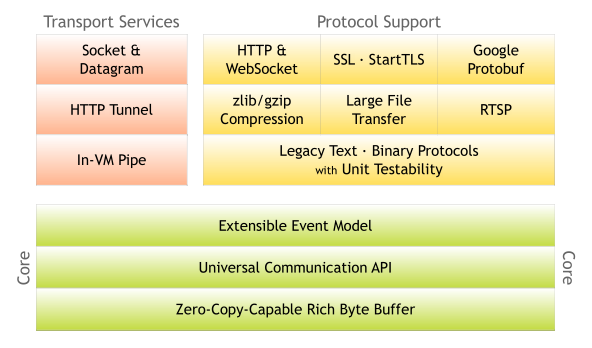
\includegraphics[width=\textwidth]{Img/netty/components.png}
  %   \caption{Kiến trúc của Netty\protect\footnotemark}
  % \end{figure}
  % \footnotetext{Nguồn: \url{https://netty.io}}
  
  \subsubsection{WebSocket}
  \textbf{Survival2D} thuộc dạng game trực tuyến nhiều người chơi (Massively Multiplayer Online - MMO), mỗi hành động của người chơi này phải được người chơi khác biết trong thời gian sớm nhất để tạo cảm giác gần như là đồng thời. Vì vậy việc trao đổi thông tin giữa client và server phải đảm bảo nhanh nhất có thể. Với mục tiêu phát triển trên nền tảng trình duyệt, nhóm lựa chọn giao thức phổ biến, dễ sử dụng và được nhiều trình duyệt hỗ trợ, đó là \textbf{WebSocket}.
  
  \textbf{WebSocket} là một giao thức truyền tin dựa trên kết nối TCP, cho phép tạo phiên giao tiếp tương tác hai chiều giữa máy khách và máy chủ. Sử dụng \textbf{WebSocket}, ta có thể gửi tin nhắn đến máy chủ và nhận các phản hồi theo hướng sự kiện mà không cần phải gửi gói tin thăm dò đến máy chủ để đợi hồi đáp. \textbf{WebSocket} hỗ trợ gói tin giao tiếp ở cả dạng text và binary; là một giao thức truyền tin dễ sử dụng, có độ trễ thấp và dễ xử lý lỗi.

  \paragraph{Ưu điểm}\mbox{}
  
  \begin{itemize}
      \item Giao thức phổ biến, dễ sử dụng, được hỗ trợ bởi nhiều trình duyệt web
      \item Hỗ trợ gói tin giao tiếp ở dạng text và binary, thích hợp kết hợp với FlatBuffers
      \item Độ trễ thấp do không phải gửi gói tin thăm dò để đợi hồi đáp
      \item Dựa trên kết nối TCP nên việc gửi nhận đảm bảo gói tin không bị thất lạc, dễ xử lý lỗi
  \end{itemize}

  \paragraph{Nhược điểm}\mbox{}
  
  \begin{itemize}
      \item Vì dựa trên kết nối TCP nên tốc độ gửi nhận chưa thể bằng UDP
  \end{itemize}

  \subsubsection{FlatBuffers}
  Để đảm bảo trải nghiệm game trực tuyến nhiều người chơi được mượt mà, cần phải đảm bảo độ trễ khi gửi/nhận gói tin là thấp nhất có thể. Phương án mà nhóm đưa ra là cố gắng giảm thiểu kích thước gói tin sao cho nhỏ nhất, để thời gian gửi ngắn đi. Và \textbf{Survival2D} có sử dụng FlatBuffers để thực hiện điều này.
  
  FlatBuffers là một thư viện thực hiện việc serialize và deserialize tương tự như Protocol Buffer (Protobuf) nhưng được đánh giá là tốt hơn.

  \paragraph{Ưu điểm}
  \begin{itemize}
      \item Nhanh hơn khi so sánh với các phương thức khác.
        \item Chỉ cần định nghĩa schema, không cần parse, unpack phức tạp như Protobuf.
        \item Hỗ trợ những trường optional.
        \item Hỗ trợ nhiều ngôn ngữ lập trình, trong đó có Java và JavaScript - 2 ngôn ngữ đang sử dụng cho server và client của \textbf{Survival2D}.
  \end{itemize} 
  
  \paragraph{Nhược điểm}
  \begin{itemize}
      \item File schema cần được định dạng, compile mới sử dụng được.
      \item Data dạng binary, không thể đọc hiểu trực tiếp. Dẫn đến khó debug hơn.
  \end{itemize}

  \begin{figure}[H]
    \centering
    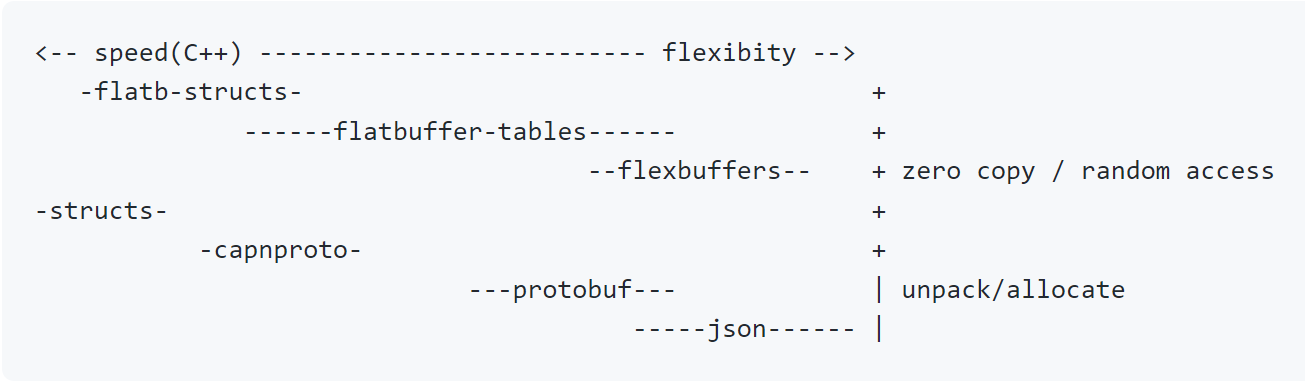
\includegraphics[width=\textwidth]{Img/flatbuffers/compare.png}
    \caption{So sánh FlatBuffers so với các phương thức khác \protect\footnotemark}
    \label{flatbuffers_compasions}
  \end{figure}
  \footnotetext{Nguồn: \url{https://github.com/google/flatbuffers/wiki/Why-FlatBuffers-vs-other-options\%3F}}

  Các bảng so sánh cho thấy FlatBuffers có hiệu năng vượt trội so với các phương thức khác, chỉ kém raw structs; lại linh động, dễ truy xuất, khắc phục được nhược điểm của raw structs.

  \begin{landscape}
\begin{table}[H]
\centering
\begin{tabular}{|c|c|c|c|c|c|c|}
\hline
\rowcolor[HTML]{374F7F} 
{\color[HTML]{FFFFFF} \textbf{}}                                                                  & {\color[HTML]{FFFFFF} \textbf{\begin{tabular}[c]{@{}c@{}}FlatBuffers\\ (binary)\end{tabular}}} & {\color[HTML]{FFFFFF} \textbf{\begin{tabular}[c]{@{}c@{}}Protocol Buffers\\ LITE\end{tabular}}} & {\color[HTML]{FFFFFF} \textbf{Rapid JSON}}                        & {\color[HTML]{FFFFFF} \textbf{\begin{tabular}[c]{@{}c@{}}FlatBuffers\\ (JSON)\end{tabular}}} & {\color[HTML]{FFFFFF} \textbf{pugixml}}                           & {\color[HTML]{FFFFFF} \textbf{Raw structs}}                   \\ \hline
\rowcolor[HTML]{FFFFFF} 
\begin{tabular}[c]{@{}c@{}}Decode + Traverse + Dealloc\\ (1 million times, seconds)\end{tabular}  & 0.08                                                                                           & 302                                                                                             & 583                                                               & 105                                                                                          & 196                                                               & 0.02                                                          \\ \hline
\rowcolor[HTML]{FFFFFF} 
\begin{tabular}[c]{@{}c@{}}Decode/Traverse/Dealloc\\ (breakdown)\end{tabular}                     & 0 / 0.08 / 0                                                                                   & 220 / 0.15 / 81                                                                                 & 294 / 0.9 / 287                                                   & 70 / 0.08 / 35                                                                               & 41 / 3.9 / 150                                                    & 0 / 0.02 / 0                                                  \\ \hline
\rowcolor[HTML]{FFFFFF} 
\begin{tabular}[c]{@{}c@{}}Encode\\ (1 million times, seconds)\end{tabular}                       & 3.2                                                                                            & 185                                                                                             & 650                                                               & 169                                                                                          & 273                                                               & 0.15                                                          \\ \hline
\rowcolor[HTML]{FFFFFF} 
\begin{tabular}[c]{@{}c@{}}Wire format size\\ (normal / zlib, bytes)\end{tabular}                 & 344 / 220                                                                                      & 228 / 174                                                                                       & 1475 / 322                                                        & 1029 / 298                                                                                   & 1137 / 341                                                        & 312 / 187                                                     \\ \hline
\rowcolor[HTML]{FFFFFF} 
\begin{tabular}[c]{@{}c@{}}Memory needed to \\ store decoded wire\\ (bytes / blocks)\end{tabular} & 0 / 0                                                                                          & 760 / 20                                                                                        & 65689 / 4                                                         & 328 / 1                                                                                      & 34194 / 3                                                         & 0 / 0                                                         \\ \hline
\rowcolor[HTML]{FFFFFF} 
\begin{tabular}[c]{@{}c@{}}Transient memory \\ allocated during decode \\ (KB)\end{tabular}       & 0                                                                                              & 1                                                                                               & 131                                                               & 4                                                                                            & 34                                                                & 0                                                             \\ \hline
\rowcolor[HTML]{FFFFFF} 
\begin{tabular}[c]{@{}c@{}}Generated source \\ code size (KB)\end{tabular}                        & 4                                                                                              & 61                                                                                              & 0                                                                 & 4                                                                                            & 0                                                                 & 0                                                             \\ \hline
\rowcolor[HTML]{FFFFFF} 
\begin{tabular}[c]{@{}c@{}}Field access in \\ handwritten traversal code\end{tabular}             & \begin{tabular}[c]{@{}c@{}}typed\\ accessors\end{tabular}                                      & \begin{tabular}[c]{@{}c@{}}typed\\ accessors\end{tabular}                                       & \begin{tabular}[c]{@{}c@{}}manual\\ error\\ checking\end{tabular} & \begin{tabular}[c]{@{}c@{}}typed\\ accessors\end{tabular}                                    & \begin{tabular}[c]{@{}c@{}}manual\\ error\\ checking\end{tabular} & \begin{tabular}[c]{@{}c@{}}typed but\\ no safety\end{tabular} \\ \hline
\rowcolor[HTML]{FFFFFF} 
\begin{tabular}[c]{@{}c@{}}Library source code \\ (KB)\end{tabular}                               & 15                                                                                             & \begin{tabular}[c]{@{}c@{}}some subset\\ of 3800\end{tabular}                                   & 87                                                                & 43                                                                                           & 327                                                               & 0                                                             \\ \hline
\end{tabular}
\caption{Bảng đánh giá hiệu năng của FlatBuffers\protect\footnotemark}
\end{table}
\footnotetext{Nguồn: \url{https://google.github.io/flatbuffers/flatbuffers\_benchmarks.html}\\
Bảng so sánh FlatBuffers với các phương thức serialization khác: \url{https://en.wikipedia.org/wiki/Comparison\_of\_data-serialization\_formats##Overview}}
\end{landscape}

  \paragraph{Ứng dụng vào Survival2D}\label{test_ping}\mbox{}

   Json là phương thức serialize phổ biến, dễ sử dụng khi phát triển các ứng dụng liên quan đến javascript và trình duyệt; vì vậy nhóm tiến hành so sánh FlatBuffers và json khi ứng dụng vào \textbf{Survival2D} để cho thấy sự hiệu quả của FlatBuffers:
   
   Các thông số được đo gồm có: kích thước gói tin và thời gian độ trễ khi truyền tải (ping time).
   
   Các gói tin được đo gồm có: Gói ping, gói player di chuyển (gói được gửi/nhận nhiều nhất game) và gói match info (gói tin có kích thước to nhất game, với thông tin của 1000 map objects và 100 players).
   
   Việc đo đạc ping time được thực hiện trên 2 môi trường: môi trường dev localhost và môi trường live (một server thật đặt tại Singapore).
   
   Thông số đo đạc được như sau:

  \begin{table}[H]
  \centering
  \begin{tabular}{|l|ll|l|}
  \hline
  \multirow{2}{*}{Gói tin} & \multicolumn{2}{l|}{Kích thước (đơn vị byte)} & \multirow{2}{*}{\begin{tabular}[c]{@{}l@{}}Tỉ lệ kích cỡ của FlatBuffers\\ khi so sánh với Json\end{tabular}} \\ \cline{2-3}
                           & \multicolumn{1}{l|}{Json}     & FlatBuffers   &                                                                                                         \\ \hline
  Ping                     & \multicolumn{1}{l|}{29}       & 36            & 124.14\%                                                                                                   \\ \hline
  PlayerMove               & \multicolumn{1}{l|}{115}      & 64            & 55.65\%                                                                                                 \\ \hline
  MatchInfo                & \multicolumn{1}{l|}{22809}    & 5396         & 23.66\%                                                                                                 \\ \hline
  \end{tabular}
  \caption{Kích thước của các gói tin quan trọng khi so sánh giữa Json và FlatBuffers}
  \textit{(Kích thước nhỏ hơn là tốt hơn)}
  \end{table}

  \begin{figure}[H]
    \centering
    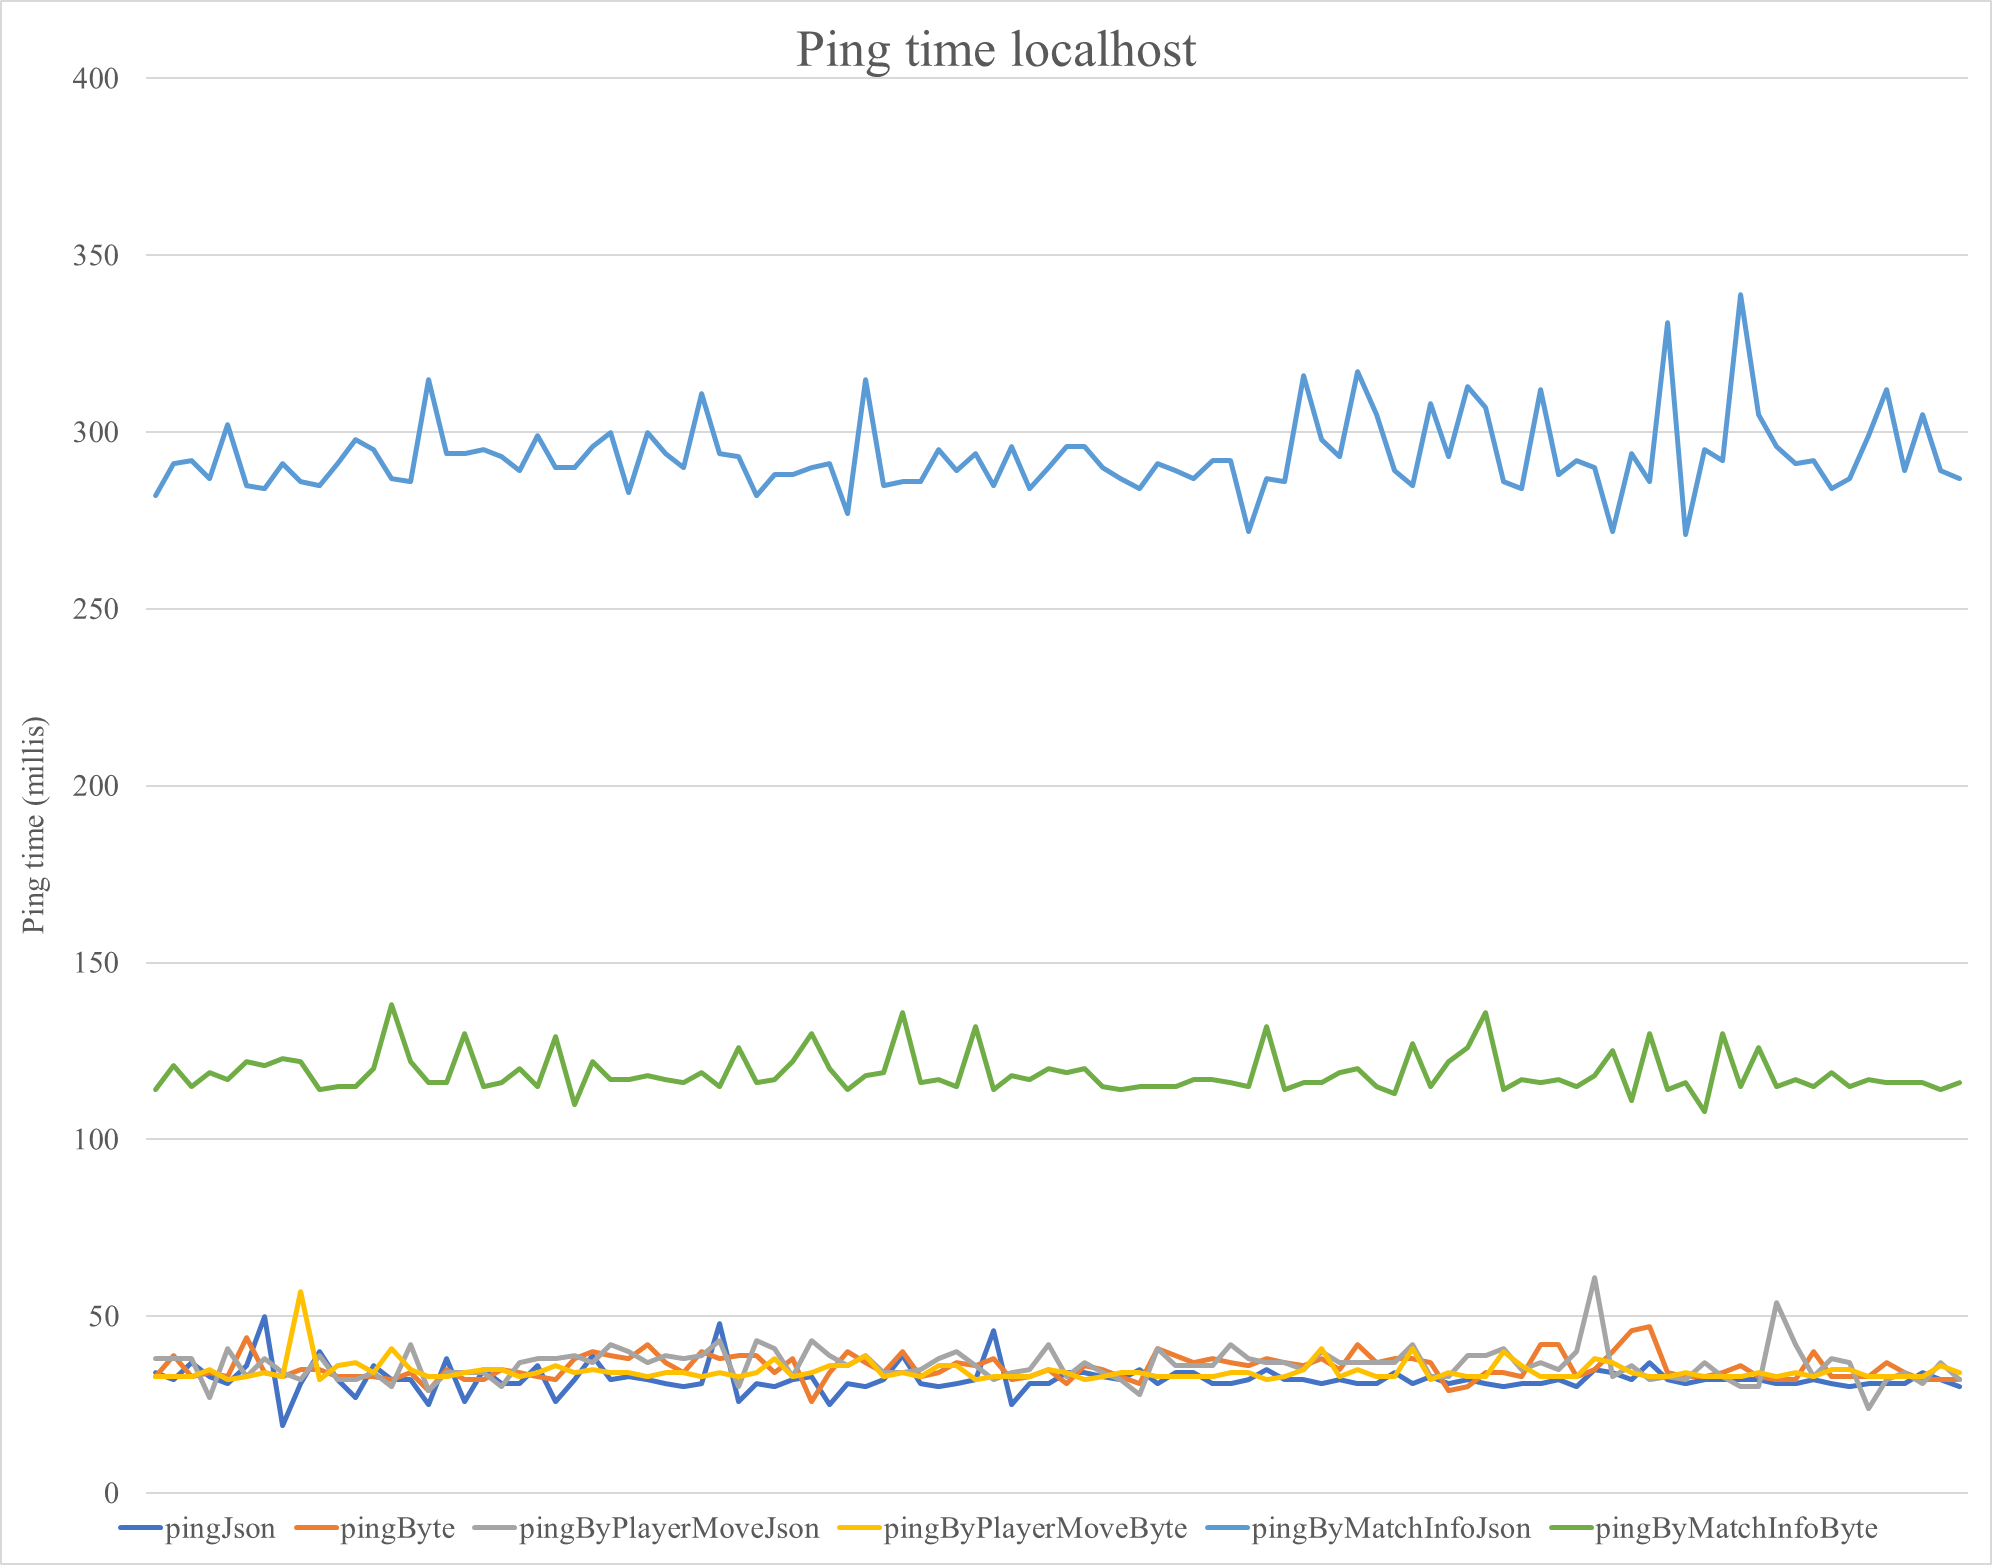
\includegraphics[width=\textwidth]{Img/flatbuffers/pinglocalhost.png}
    \caption{Biểu đồ độ trễ của các gói tin khi so sánh trên localhost}
  \end{figure}

  \begin{table}[H]
  \centering
  \begin{tabular}{|l|ll|l|}
  \hline
  \multirow{2}{*}{Gói tin} & \multicolumn{2}{l|}{Ping time trung bình (đơn vị millis)} & \multirow{2}{*}{\begin{tabular}[c]{@{}l@{}}Tỉ lệ ping time của FlatBuffers\\ khi so sánh với Json\end{tabular}} \\ \cline{2-3}
                           & \multicolumn{1}{l|}{Json}   & FlatBuffers &                                                                                                            \\ \hline
  Ping                     & \multicolumn{1}{l|}{32.28}  & 35.53       & 110.07\%                                                                                                   \\ \hline
  PlayerMove               & \multicolumn{1}{l|}{36.35}  & 34.41       & 94.66\%                                                                                                    \\ \hline
  MatchInfo                & \multicolumn{1}{l|}{293.24} & 118.7       & 40.48\%                                                                                                    \\ \hline
  \end{tabular}
  \caption{Độ trễ (ping time) trung bình của các gói tin quan trọng khi so sánh giữa Json và FlatBuffers trên môi trường localhost}
  \textit{(Độ trễ nhỏ hơn là tốt hơn)}
  \label{pinglive}
  \end{table}

  \begin{figure}[H]
    \centering
    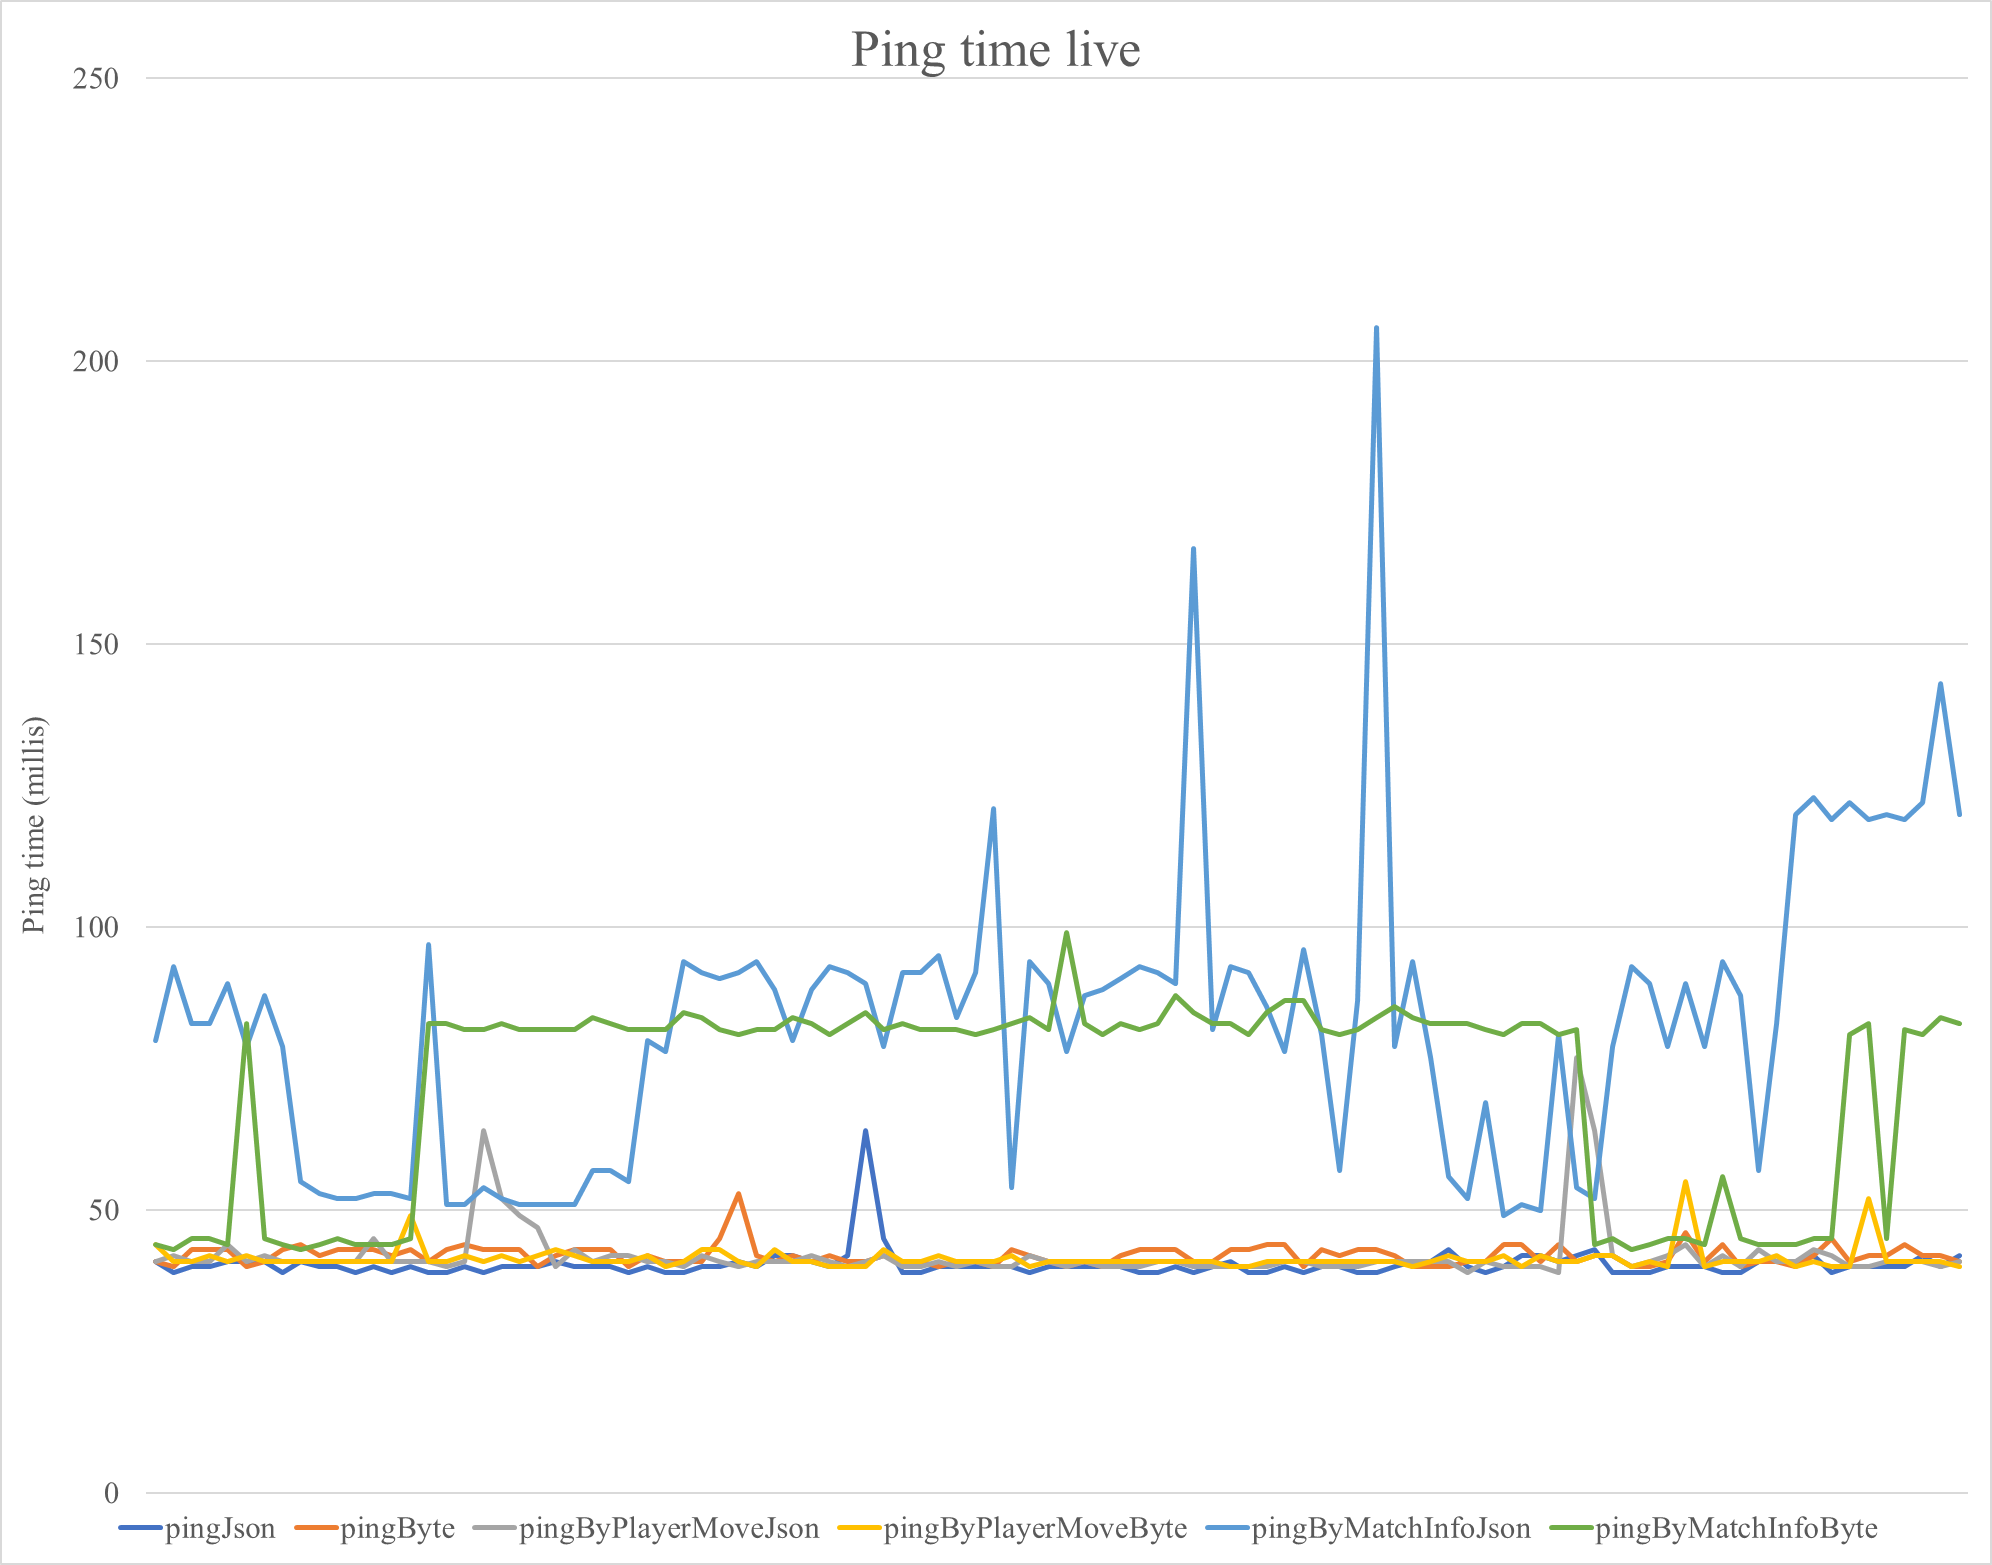
\includegraphics[width=\textwidth]{Img/flatbuffers/pinglive.png}
    \caption{Biểu đồ độ trễ của các gói tin khi so sánh trên server thật đặt tại Singapore}
  \end{figure}

  \begin{table}[H]
  \centering
  \begin{tabular}{|l|ll|l|}
  \hline
  \multirow{2}{*}{Gói tin} & \multicolumn{2}{l|}{Ping time trung bình (đơn vị millis)} & \multirow{2}{*}{\begin{tabular}[c]{@{}l@{}}Tỉ lệ ping time của FlatBuffers\\ khi so với Json\end{tabular}} \\ \cline{2-3}
                           & \multicolumn{1}{l|}{Json}           & FlatBuffers         &                                                                                                            \\ \hline
  Ping                     & \multicolumn{1}{l|}{40.4}           & 42.03               & 104.03\%                                                                                                   \\ \hline
  PlayerMove               & \multicolumn{1}{l|}{42}             & 41.44               & 98.67\%                                                                                                    \\ \hline
  MatchInfo                & \multicolumn{1}{l|}{83.39}          & 71.93               & 86.26\%                                                                                                    \\ \hline
  \end{tabular}
  \caption{Độ trễ (ping time) trung bình của các gói tin quan trọng khi so sánh giữa Json và FlatBuffers trên server thật đặt tại Singapore}
  \textit{(Độ trễ nhỏ hơn là tốt hơn)}
  \end{table}
  
  Các so sánh trên cho thấy được FlatBuffers đã giúp \textbf{Survival2D} giảm packet size và ping time đáng kể. Gói tin càng lớn thì độ hiệu quả của FlatBuffers càng cao. Điều này rất thích hợp để phát triển \textbf{Survival2D} thêm, vì khi đó số lượng gói tin lẫn kích thước gói tin sẽ ngày càng tăng.
  
  \newpage
  \section{Phân tích hệ thống}
  Tổng quan về hệ thống game, muốn phát triển \textbf{Survival2D} với những tính năng đáp ứng mục tiêu đề ra, trước hết ta cần phải có một môi trường gameplay cơ bản. Một gameplay chiến đấu sẽ có các phần chính đó là bản đồ (map), người chơi (player) và các đối tượng khác (objects), vật phẩm người chơi như súng, đạn,...
  
  Từ đó, nhóm đưa ra phân tích về hệ thống cần thiết kế của game có những vấn đề quan trọng bao gồm:
  \begin{itemize}
      \item Bản đồ (Map), và các đối tượng trên map: cách tạo ra map và quản lý các đối tượng hiệu quả.
      \item Giải pháp để hạn chế hack/cheat.
      \item Hiện thực người chơi máy (bot).
  \end{itemize}
  \subsection{Bản đồ (Map)}
  Bản đồ (map) là một mô phỏng của chiến trường, nơi mà các người chơi sẽ đối đầu với nhau trực tiếp ở trên đó. Là game chiến đấu thời gian thực nhiều người chơi nên map là một phần rất quan trọng ảnh hưởng đến chất lượng và sự hấp dẫn của game. Do đó, việc có một hệ thống tạo và quản lý map hiệu quả là rất cần thiết.
  
  Một số vấn đề của khâu thiết kế và quản lý map có thể kể đến như là độ rộng của map, quản lý logic map, hiển thị map, thiết kế vật thể trên map (map object),...
  \begin{figure}[H]
      \centering
      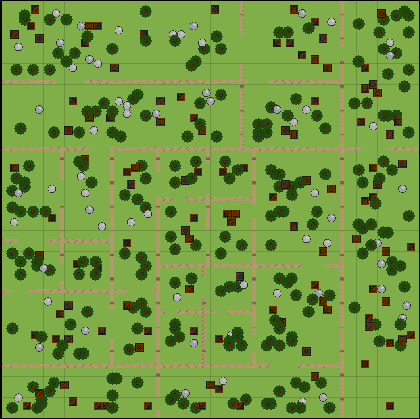
\includegraphics{Img/tilemaps/Main_Small_Map.png}
      \caption{Bản đồ tổng thể trong \textbf{Survival2D} \cite{bib16}}
  \end{figure}
  \subsubsection{Map lớn}
  Để mô phỏng chiến trường 2D mà trong đó có 100 người chơi được phân bố vị trí đảm bảo cách xa nhau, ta cần có một map với diện tích đủ rộng. Ví dụ một người chơi chiếm diện tích 1 $m^2$ được quy đổi vào game là 1 cell, người chơi được sinh ra ở vị trí an toàn là trong phạm vi bán kính 100 cells không có địch, ta tạm xem như một vùng an toàn như vậy có diện tích 100 x 100 cells, 100 vùng như vậy tương đương 100 x 100 x 100 = 1000000 cells, vậy có nghĩa là map có diện tích khoảng 1000000 cells. Lúc này game sẽ gặp hai vấn đề cần giải quyết:
  \begin{itemize}
    \item Hiển thị map (client): Với máy tính sử dụng 16-bit màu, mỗi pixel sẽ dùng 4 bits để hiển thị màu sắc của chúng, tương tự sẽ là 8 bits đối với 32-bit màu. Ví dụ mỗi cell tương ứng 32 x 32 pixels, 1000000 cells tương ứng 32 x 32 x 1000000 = 1024000000 pixels, lúc này để hiển thị được toàn bộ map, ta cần khoảng 488 megabytes đối với 16-bit màu và khoảng gần 1 gigabytes đối với 32-bit màu, thực sự lớn.
    \item Xử lý logic trên map (chủ yếu với server): Nếu xử lý logic trên toàn map, ta phải xử lý cho hàng trăm người chơi và rất nhiều những đối tượng khác trên map như đạn, súng, vật phẩm, vật cản,... cùng một lúc. Ví dụ trong một game có 100 người chơi, tương tác nhặt súng nhặt đạn, sau đó giả sử mỗi người bắn 2-3 viên đạn -> số lượng object lên đến 150-200 objects (chưa tính vật cản), vậy số phép tính toán là cực lớn.
  \end{itemize}
  \subsubsection{Các đối tượng trên map (map objects)}
  Trong game, ngoài người chơi thì ta còn có những objects khác bao gồm đạn, vật phẩm, vật cản như cây, đá, tường,...(hình \ref{mapobjects}) 

  \begin{figure}[H]
      \centering
      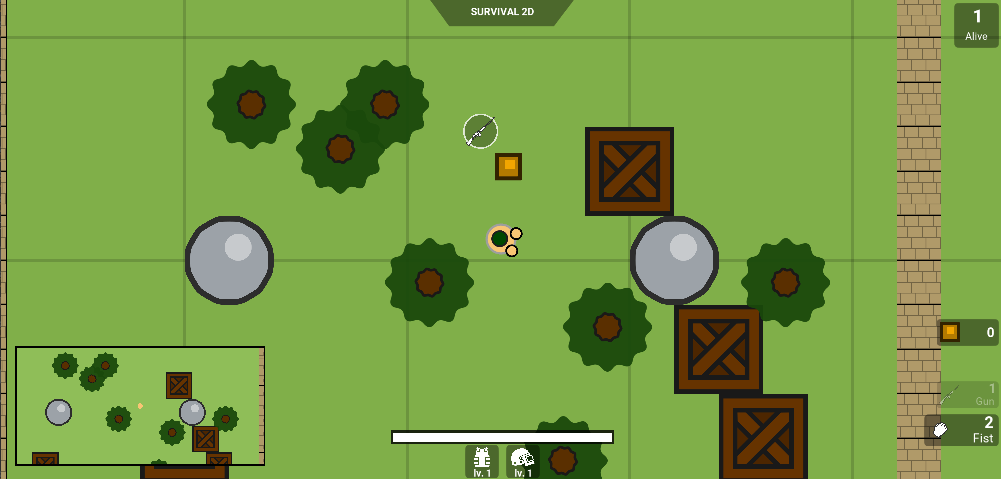
\includegraphics[width=\textwidth]{Img/map/objects.png}
      \caption{Các objects trong \textbf{Survival2D}}
      \label{mapobjects}
  \end{figure}
  
  Tuỳ vào loại object mà chúng sẽ có những logic cần phải xử lý khác nhau. Để quản lý tốt chúng, ta cũng sẽ phải có một hệ thống quản lý map objects, hệ thống đó cần đáp ứng được những vấn đề sau:
  \begin{itemize}
      \item Nhiều loại object, số lượng objects lớn.
      \begin{itemize}
          \item Các object trong game sẽ được phân thành nhiều lớp và có những thuộc tính, hành vi nhất định.
          \item Một số lớp sẽ có số object cố định, nhưng một số lớp thì không, và thậm chí là số lượng còn là rất lớn, sinh ra, tồn tại, mất đi liên tục và có thể gần như cùng lúc trong một số trường hợp.
      \end{itemize}
      \item Các objects tương tác với nhau chặt chẽ.
  \end{itemize}
  
  \subsubsection{Thiết kế (design) map}
  Bản thân của map cũng là một object của game, cũng sẽ được thiết kế logic và có hệ thống quản lý như các objects khác. Tuy nhiên vẫn còn vấn đề về design map nữa đó là việc ta phải thiết kế tất cả các thuộc tính của map như là hình dạng, độ rộng, vị trí objects phân bố trên map, thời gian chúng xuất hiện,...
  
  Để game thu hút người chơi, map còn đòi hỏi các vật cản được sắp xếp tự nhiên, hợp lý; các vật phẩm xuất hiện phải cân bằng, không thiên vị cho một player nào. Bên cạnh đó map cũng phải liên thông được, tránh player bị kẹt, không có cách nào để di chuyển đển khu vực khác trên bản đồ.
  
  Với map có diện tích lớn như 10000x10000 pixels của \textbf{Survival2D}, việc thiết kế đảm bảo tất cả các yêu cầu trên là một vấn đề khó.
  
  \subsection{Người chơi máy (bot)}
  Người chơi máy (bot) là một phần hầu như không thể thiếu trong khá nhiều thể loại game và đặc biệt là game chiến đấu. Trong nhiều trường hợp, sự thể hiện của người chơi máy có ảnh hưởng rất lớn tới sự thành công của game. Lấy ví dụ, khi game không có nhiều người chơi đang chơi cùng lúc do nhiều lý do khác nhau (game chưa thu hút nhiều người chơi, thời điểm ít người chơi trong ngày,...) thì bot sẽ giúp cho game vẫn giữ được sự nhộn nhịp và đảm bảo cho trận đấu vẫn có thể diễn ra hấp dẫn.
  
  Có nhiều vấn đề về việc thiết kế bot, ví dụ như làm sao để bot di chuyển thông minh, tự nhiên, hành vi giống như người chơi thật trong vài tình huống, bên cạnh đó lại không quá áp đảo người chơi để giữ cho người chơi cảm giác hưng phấn,... Thiết kế bot cũng là một vấn đề khó.
  
  \subsection{Hạn chế hack}
  Một trong những vấn đề lớn của game online là nạn hack/cheat. Hack cheat làm mất cân bằng game, gây bất lợi cho người chơi không dùng hack, từ đó người chơi dễ nản chí và bỏ game; khi đó tổng lượng người chơi giảm, người chơi hack cũng sẽ không gắn bó với game lâu dài, lại làm mất uy tín của nhà phát hành, ảnh hưởng đến các sản phẩm khác. Vì vậy cơ chế bảo mật để chống hack cũng là một vấn đề khó và quan trọng không kém.
  
  \subsubsection{Hạn chế hack ESP \textit{(Extra Sensory Perception)}}
  
  Hack map, hack ESP, hack xuyên tường,... là các thể loại hack phổ biến trên các game bắn súng. Những tựa game bắn súng nổi tiếng như PUBG, CS:GO, Valorant,... đều bị các vấn nạn hack kể trên.
  \paragraph{Nguyên nhân:}\mbox{}
  
  Do các thông tin cần biết để biểu diễn, render ở client quá lớn, ví dụ người chơi ở bên kia tường khi di chuyển ta sẽ nghe tiếng chân; người chơi nấp sau tường nhưng vẫn sẽ có đổ bóng; người chơi ở quá xa, khi bắn súng ta vẫn nhìn thấy tia lửa,... Client cần biết thông tin như người chơi đó đang đứng hay ngồi, quay mặt về hướng nào,... để biểu diễn cho chính xác. Dẫn đến server phải gửi rất nhiều thông tin người chơi khác (mà về mặt logic người chơi không được biết) để client hiển thị cho đúng. Các modder tận dụng lỗ hổng này khai thác, lấy những thông tin bị che dấu đi này để làm các bản hack cho người chơi biết trạng thái của người chơi khác, gọi là hack ESP.

  Ví dụ trong hình \ref{cheat_esp_pubgm}, người chơi thấy được vị trí đối thủ dù bị khuất tầm nhìn, có được lợi thế khi giao tranh.
  \begin{figure}[H]
    \centering
    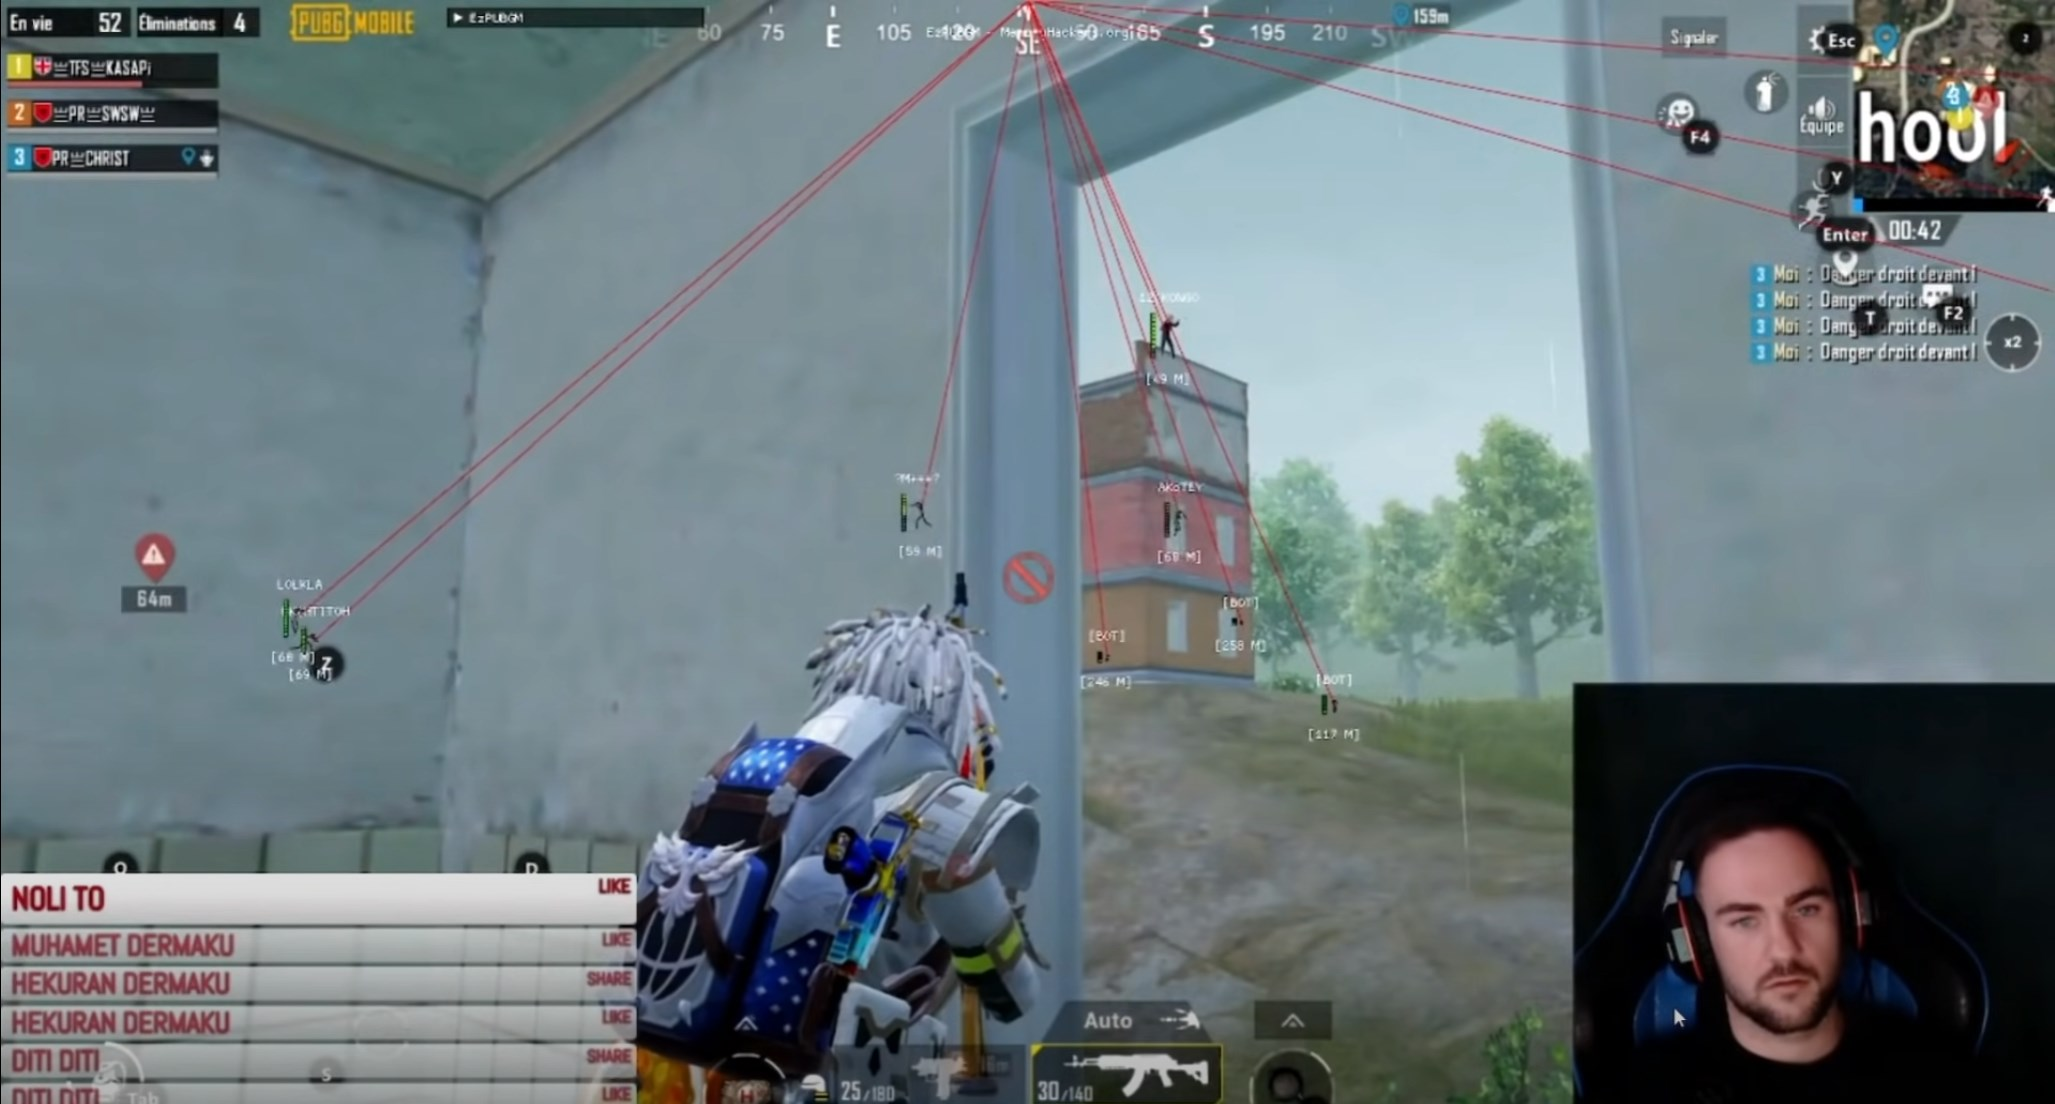
\includegraphics[width=\textwidth]{Img/cheat/cheat_esp_pubgm.jpg}
    \caption{Người chơi cheat ESP trong game PUBG Mobile\protect\footnotemark}
    \label{cheat_esp_pubgm}
  \end{figure}
  \footnotetext{Nguồn: \url{https://www.youtube.com/watch?v=v8Cwrn-waf4}}
  
  \paragraph{Cách khắc phục ở Survival2D:}\mbox{}
  
  Do \textbf{Survival2D} là game 2D đơn giản, những logic quản lý thông tin về vùng nhìn thấy của người chơi rất dễ thực hiện, nên server sẽ tính toán luôn phần này thay client.
  
  Ví dụ trong hình \ref{antihackesp}: Người chơi P1 đứng dưới tán cây, có vùng nhìn màu xanh. Người chơi P2 đứng ngoài tán cây, có vùng nhìn màu cam. Vùng nhìn của người chơi P2 bị che mất đi các vật thể ở bên dưới tán cây. Lúc server gửi thông tin trong vùng nhìn về cho người chơi P2 sẽ lược bỏ các thông tin nằm dưới tán cây, do đó người chơi P2 sẽ không biết gì về người chơi P1. Còn khi server thông tin về cho người chơi P1, thì sẽ gửi luôn thông tin của người chơi P2 do không bị cản trở. Điều này cũng áp dụng cho các công trình gây cản trở tầm nhìn khác ví dụ nhà, hầm,... và các object di chuyển trên map (ví dụ người chơi, đạn,...). Cơ chế này làm cho modder không thể hack ESP được.
  
  \begin{figure}[H]
    \centering
    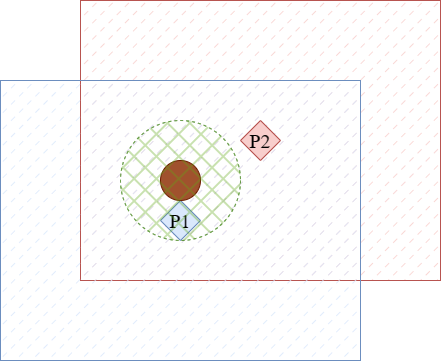
\includegraphics[width=0.7\textwidth]{Img/anticheat/PlayerView.png}
    \caption{Mô tả cơ chế chống hack ESP bằng vùng nhìn trong \textbf{Survival2D}}
    \label{antihackesp}
  \end{figure}
  
  \subsubsection{Hạn chế các hack khác}
  Các trường thông tin người chơi như tên, máu, lượng đạn,... của người chơi đều được xác thực thông qua session của người chơi, vì vậy sẽ không thể có việc người chơi B có thể can thiệp vào thông tin của người chơi A.
  
  Các thông tin hiển thị ở client, về máu, súng, lượng đạn, sát thương của súng... của bản thân và đối thủ đều là do server trả về, vì vậy các giá trị trong bộ nhớ của client chỉ mang tính chất dùng để hiển thị trên game. Dù modder có thay đổi giá trị này thì cũng chỉ có thể làm hiển thị ở client của bản thân sai khác đi chứ không ảnh hưởng đến logic thật sự của server gửi cho những client khác.
  
  \newpage
  \section{Thiết kế hệ thống}
  Từ những phân tích ở phần trước, nhóm đưa ra các giải pháp tương ứng cho các vấn đề đặt ra như sau:
  \begin{itemize}
      \item Thiết kế hệ thống quản lý map
      \begin{itemize}
          \item Thiết kế map
          \item Thiết kế objects và hệ thống quản lý objects
          \item Sinh map ngẫu nhiên
      \end{itemize}
      \item Thiết kế mô hình client-server
      \begin{itemize}
          \item Thiết kế cơ bản
          \item Kỹ thuật dự đoán phía client
      \end{itemize}
      \item Thiết kế người chơi máy (bot)
      \begin{itemize}
          \item Thuật toán tìm đường đi cho bot
          \item Xây dựng cây hành vi (behavior tree) quản lý hành vi cho bot
          \item Thiết kế độ khó cho bot
      \end{itemize}
  \end{itemize}
  \subsection{Thiết kế hệ thống quản lý map}
  \subsubsection{Thiết kế map}
  Map được thiết kế theo góc nhìn từ trên xuống (top-down), và các objects map cũng sẽ được chiếu lên map theo góc nhìn như vậy.
  \begin{itemize}
      \item Quản lý map và các objects map bằng ma trận hai chiều.

      Một ma trận 2 chiều tương ứng với hệ trục toạ độ \textit{Oxy}, được sử dụng để mô phỏng map và quản lý vị trí cũng như kích thước của toàn bộ các đối tượng có trên map.
      
      \item Load map từng phần.
      
      Thay vì load toàn bộ map (objects map) ngay từ đầu, map sẽ được load từng phần theo từng khu vực mà người chơi đang nhìn thấy, điều này sẽ giúp tăng tốc độ tính toán hơn và giảm thời gian chờ khởi tạo trận đấu. Khi người chơi vào trận, ta có thể biết vị trí hiện tại của người chơi và dựa vào đó, phần map đầu tiên sẽ được load, các objects ở quanh khu vực đó được tạo ra. Khi người chơi di chuyển, tuỳ vào vị trí của người chơi mà các phần khác sẽ được load tiếp theo. Khi load từng phần như vậy, phần map được load là một vùng lớn hơn vùng nhìn tối đa của người chơi, để không gây hiện tượng các objects tạo ra bị chậm khi người chơi đã di chuyển đến đó.
      
      \item Chia nhỏ map, quản lý theo từng đoạn (chunk).
      
      Tương tự hiển thị map trên client, phần xử lý logic ta cũng có thể chia nhỏ map theo chunks, và chỉ quản lý logic trên từng vùng rồi kết nối chúng lại với nhau. Mỗi người chơi ở trong chunk sẽ đăng ký theo dõi các sự kiện của chunk đó, khi di chuyển qua khu vực khác thì sẽ huỷ đăng ký với chunk cũ và lại đăng ký vào chunk mới. Với phương án này, khi có các sự kiện diễn ra ở mỗi chunk, ta chỉ cần xử lý sự kiện đó trong chính chunk đó mà không cần duyệt toàn map hay broadcast cho toàn bộ người chơi khác trên map, vừa giảm được khối lượng tính toán mà vừa giúp game có tính bảo mật, chống cheat khiến người chơi không thể biết được những sự kiện xảy ra ở ngoài vùng nhìn thấy của người chơi đó.
  \end{itemize}
  
  \subsubsection{Thiết kế và quản lý các objects}
  \paragraph{Thiết kế class diagram của các objects}\mbox{}

  Các object trong một trận đấu của Survival2D được thiết kế theo hướng đối tượng (OOP), kết hợp với design patterns thích hợp.

  Nhận thấy một số thuộc tính tồn tại ở nhiều class, và các thuộc tính này có tính chất, hành động giống nhau. Nhóm đã định nghĩa ra nhiều interface phổ biến để các class khác kế thừa. Và do java không cho phép đa kế thừa, nhóm đã hiện thực những method dùng chung này bằng tính năng default method của java.
  
  Ví dụ: Interface \textit{HasHp} và \textit{Destroyable} không liên quan đến nhau. class \textit{Container} do có thể bị phá huỷ nên sẽ hiện thực interface \textit{Destroyable}; nhưng \textit{Container} khi bị đánh sẽ hao mòn dần chứ không bị phá huỷ ngay, nên sẽ hiện thực interface \textit{HasHp} để thể hiện "độ bền". Khi bị đánh, \textit{Container} sẽ gọi \textit{reduceHp} của \textit{HasHp}, và để hiện thực \textit{isDestroyed} của \textit{Destroyable}, \textit{Container} sẽ gọi \textit{isDestroyed} của \textit{HasHp}, chứ không phải hiện thực lại. Code bên dưới mô tả cho ví dụ này, các class, field và method không liên quan đã được ẩn đi để tránh nhầm lẫn.

  \begin{lstlisting}[language=java]
public interface HasHp {

  double getHp();

  void setHp(double hp);

  default void reduceHp(double hp) {
    setHp(getHp() - hp);
  }

  default boolean isAlive() {
    return getHp() > 0;
  }

  default boolean isDestroyed() {
    return !isAlive();
  }
}
  \end{lstlisting}

  \begin{lstlisting}[language=java]
public interface Destroyable {
  void setDestroyed(boolean destroyed);
  
  boolean isDestroyed();
  
  default void markDestroyed() {
    setDestroyed(true);
  }
}
  \end{lstlisting}

    \begin{lstlisting}[language=java]
//Irrelevant classes, fields and methods have been hidden
public class Container implements Destroyable, HasHp {
  double hp;

  @Override
  public boolean isDestroyed() {
    return HasHp.super.isDestroyed();
  }
}
  \end{lstlisting}

  Nhờ mô hình trên mà \textbf{Survival2D} chỉ hiện thực logic 1 lần ở interface chung, tránh bị trùng lặp code.
  
  Class diagram cho các lớp (class) quan trọng trong một trận đấu như sau:

  \begin{sidewaysfigure}[H]
    \centering
    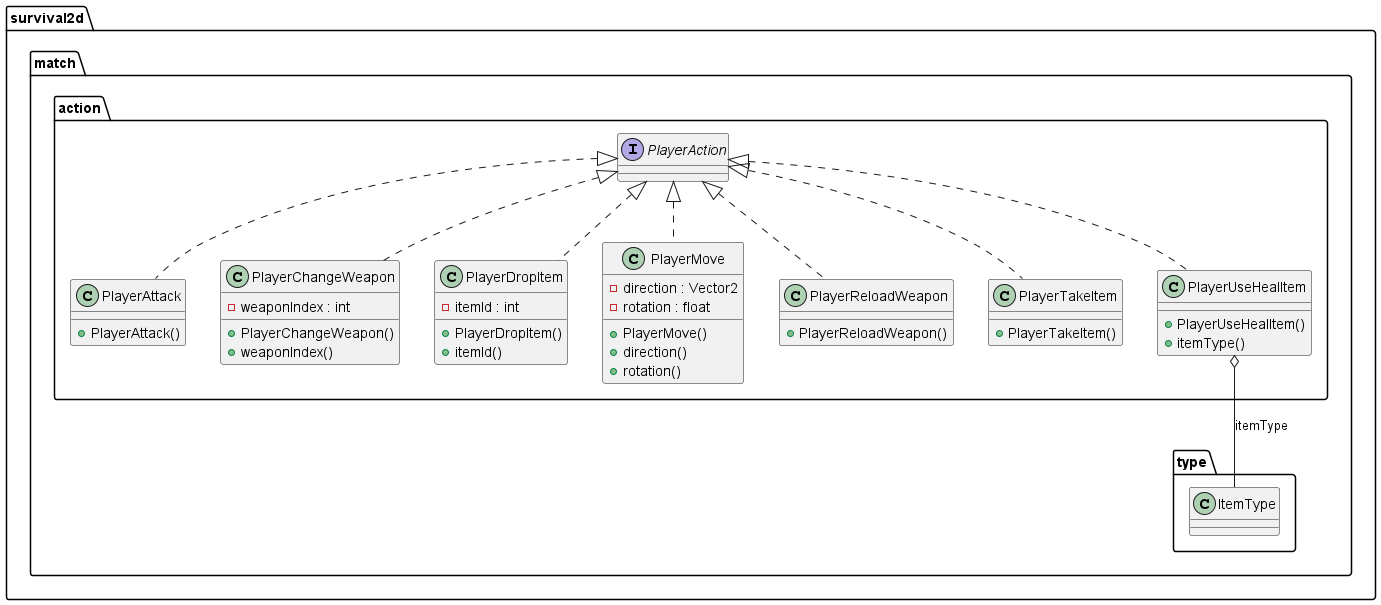
\includegraphics[width=\textwidth]{Img/uml/action.png}
    \caption{Diagram các action của player}
  \end{sidewaysfigure}

  \begin{figure}[H]
    \centering
    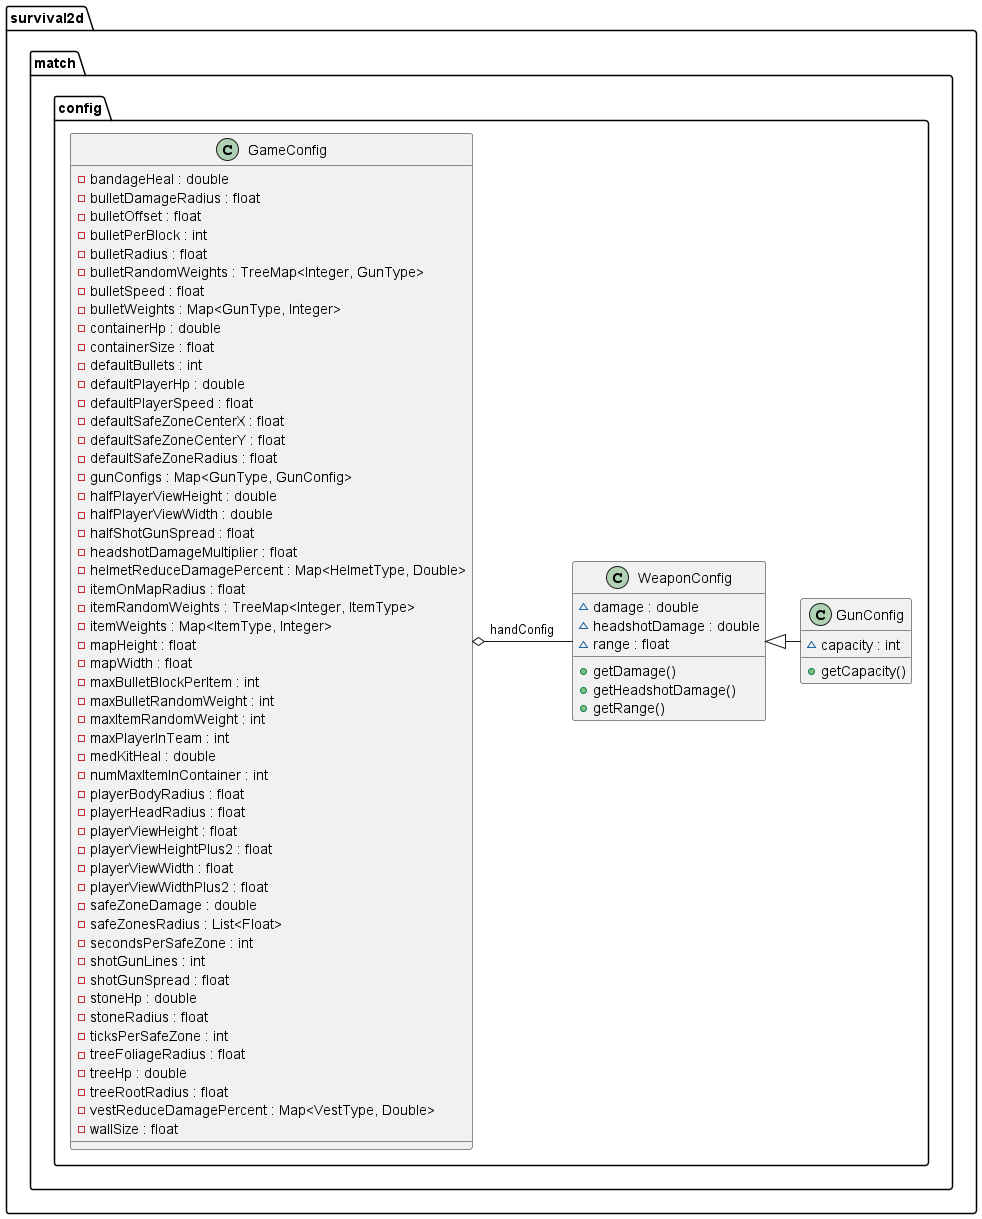
\includegraphics[width=\textwidth,height=0.95\textheight,keepaspectratio]{Img/uml/config.png}
    \caption{Diagram của class GameConfig, chứa các config cần thiết trong game}
  \end{figure}
  
  \begin{figure}[H]
    \centering
    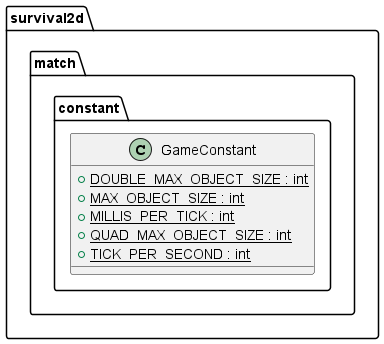
\includegraphics[width=0.6\textwidth]{Img/uml/constant.png}
    \caption{Diagram của class GameConstant, chứa các thông số sẽ không bao giờ đổi trong game}
  \end{figure}

  \begin{figure}[H]
    \centering
    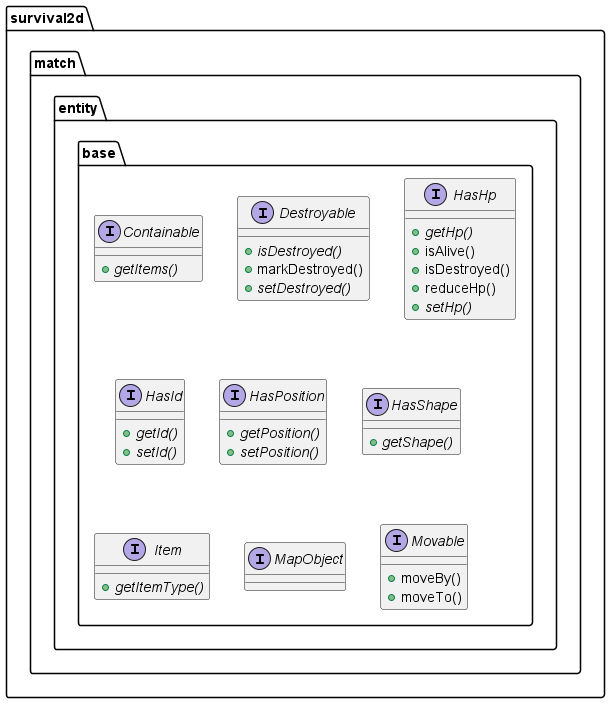
\includegraphics[width=0.8\textwidth]{Img/uml/base.png}
    \caption{Diagram của các class cơ bản}
    Các interface này sẽ được các class khác kế thừa và tận dụng logic đã hiện thực.
  \end{figure}

  \begin{sidewaysfigure}
    \centering
    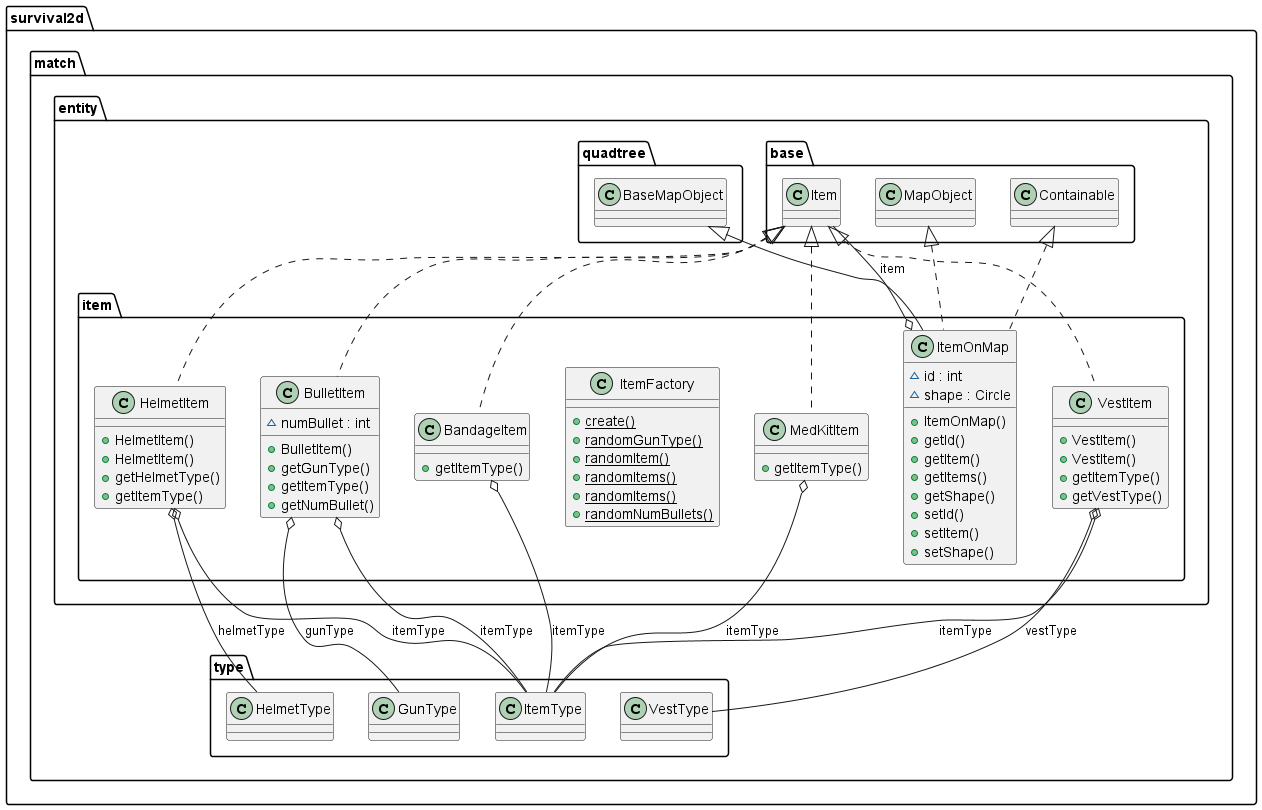
\includegraphics[width=\textwidth]{Img/uml/item.png}
    %Có tricky ở đây, các item type nằm ở package base chứ không trong item
    \caption{Diagram của các item}
    Các item sẽ có method getItemType để biết loại item; và có thêm type cụ thể của từng loại item (như GunType, BulletType,...).
  \end{sidewaysfigure}

  \begin{figure}[H]
    \centering
    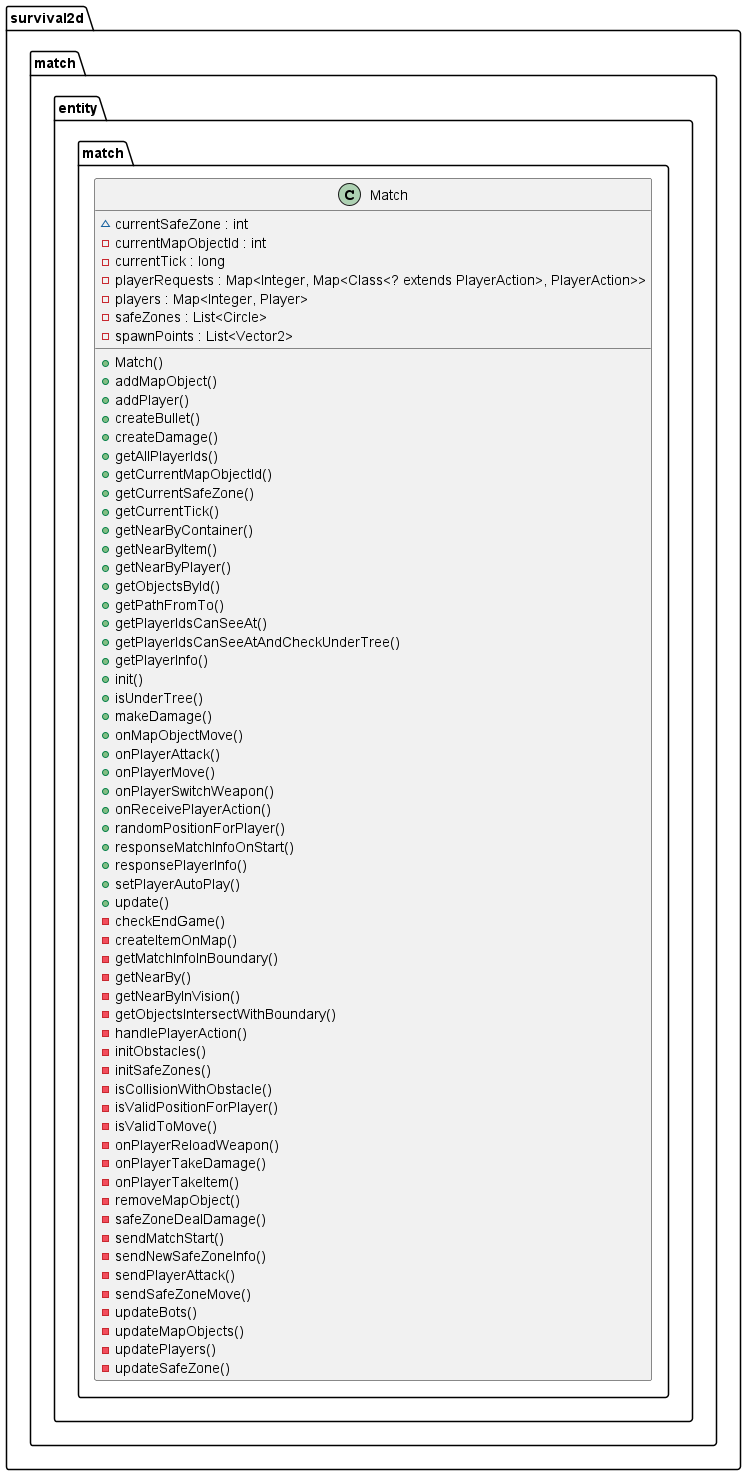
\includegraphics[width=\textwidth,height=0.95\textheight,keepaspectratio]{Img/uml/match.png}
    \caption{Diagram của trận đấu}
    Trận đấu chứa thông tin của toàn bộ objects trong một game, cũng là nơi thực thi logic game.
  \end{figure}

  \begin{sidewaysfigure}
    \centering
    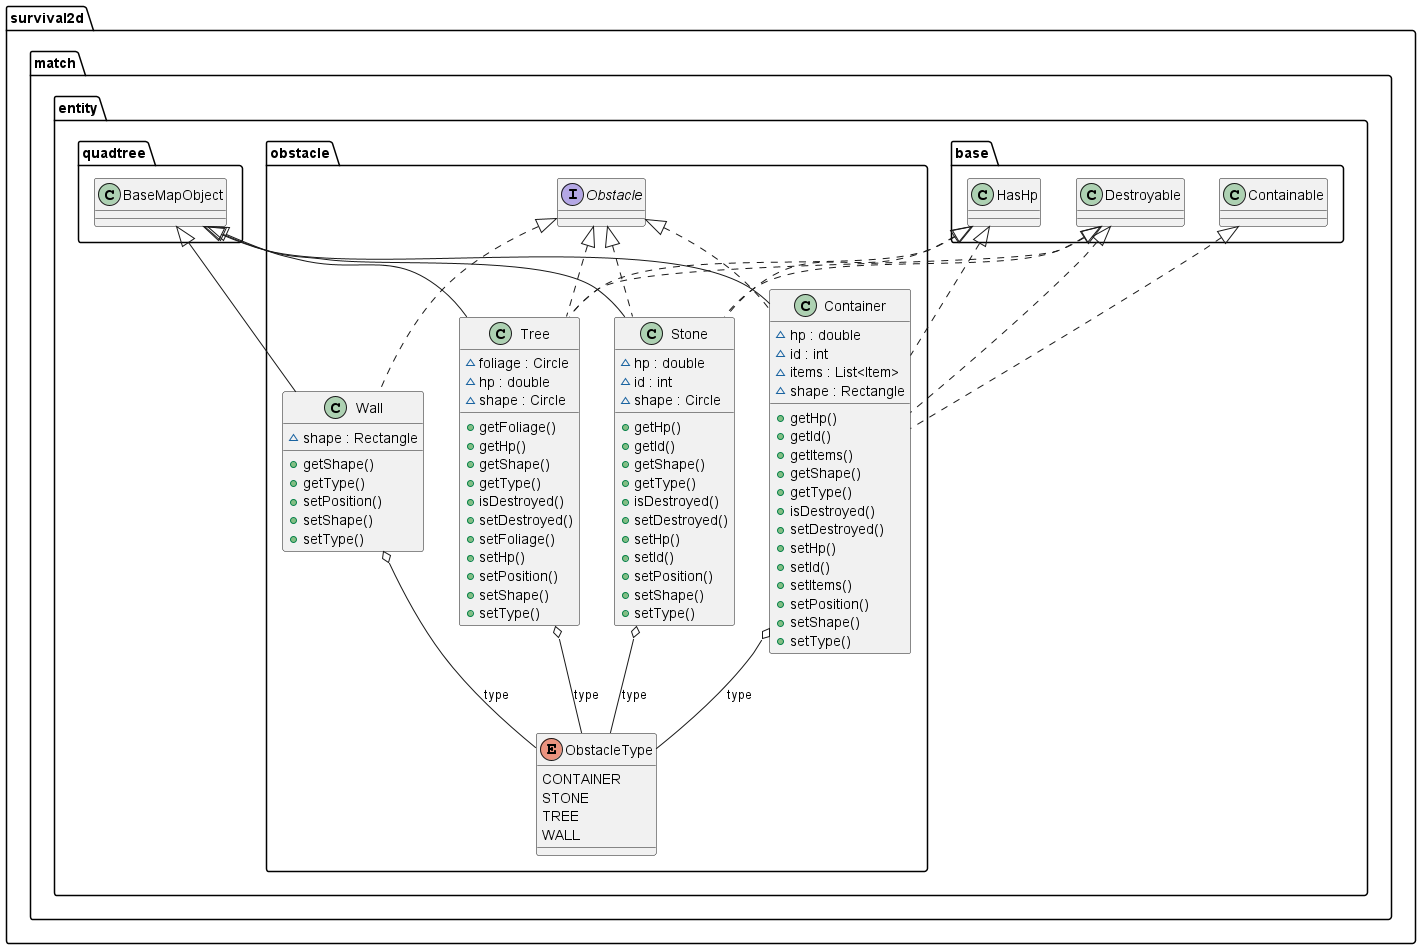
\includegraphics[width=0.9\textwidth]{Img/uml/obstacle.png}
    \caption{Diagram của các vật cản}
    Các vật cản của \textbf{Survival2D} tuy ít nhưng mỗi loại vật cản lại mang vai trò riêng biệt.
  \end{sidewaysfigure}

  \begin{figure}[H]
    \centering
    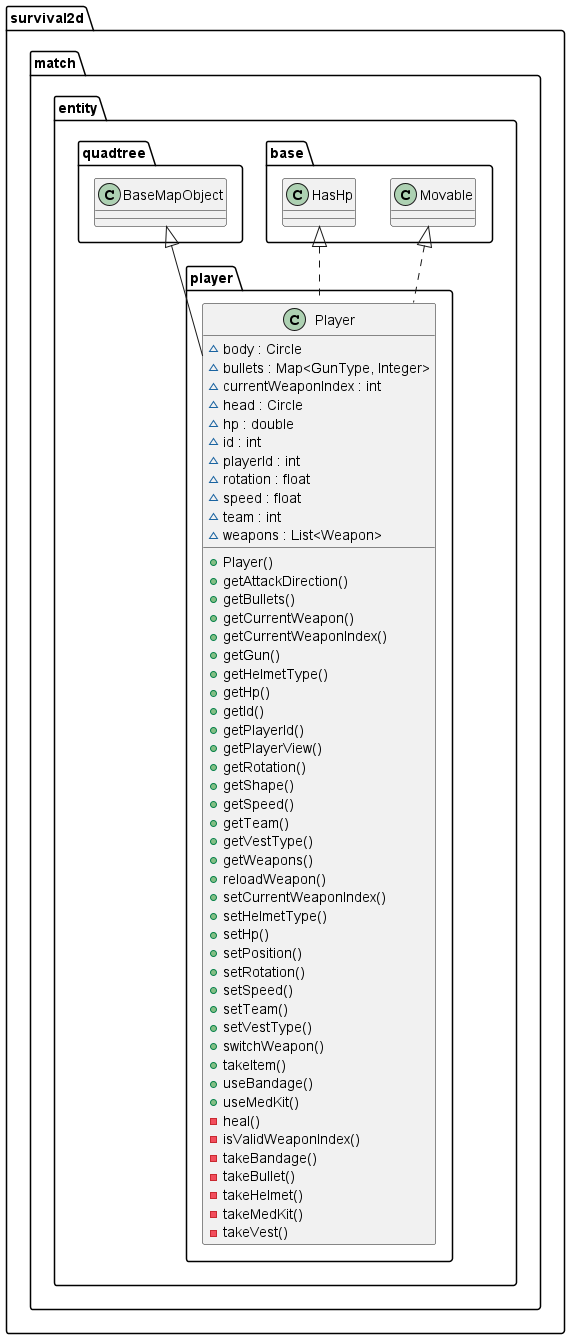
\includegraphics[width=\textwidth,height=0.95\textheight,keepaspectratio]{Img/uml/player.png}
    \caption{Diagram của player}
    Class Player chứa nhiều thông tin về vũ khí, trang bị mà người chơi đang nắm giữ.
  \end{figure}

  \begin{figure}[H]
    \centering
    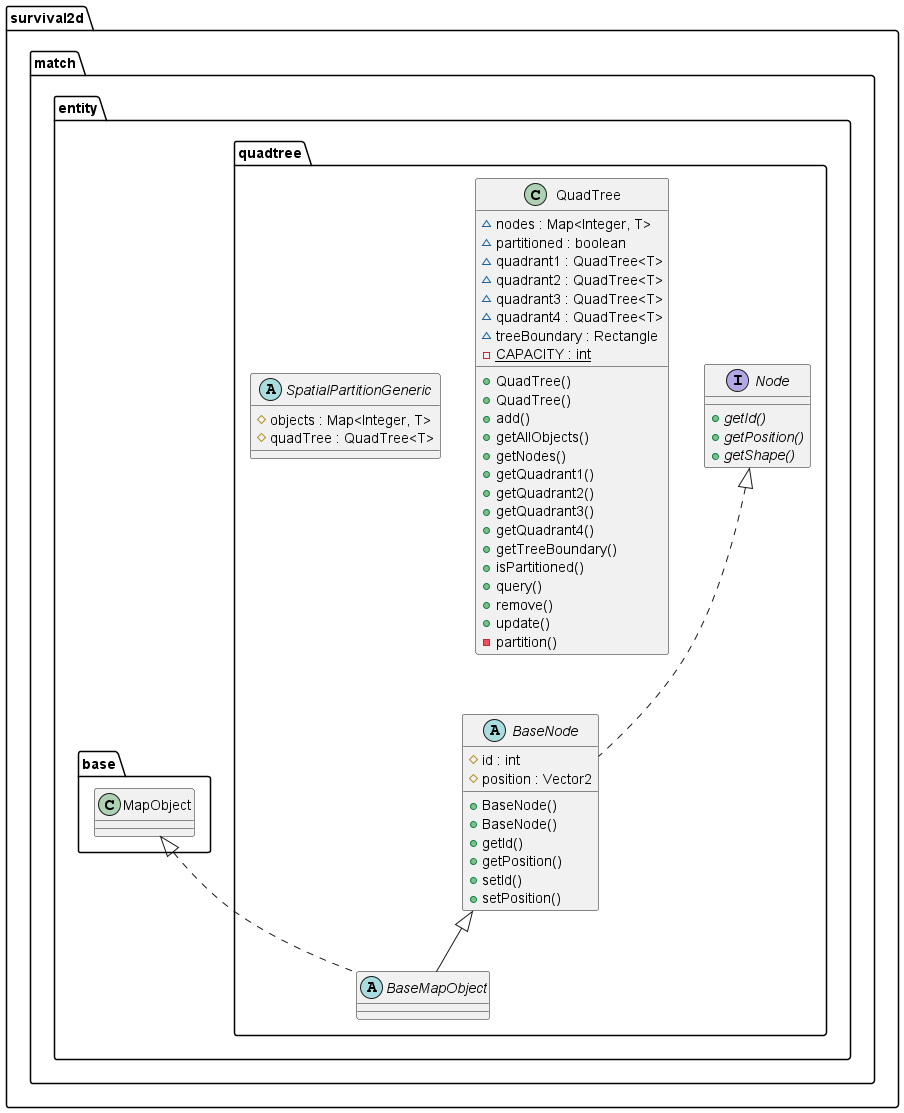
\includegraphics[width=\textwidth,height=0.9\textheight,keepaspectratio]{Img/uml/quadtree.png}
    \caption{Diagram của quadtree}
    Các class này dùng để cải thiện truy xuất object trong match.
  \end{figure}

  \begin{figure}[H]
    \centering
    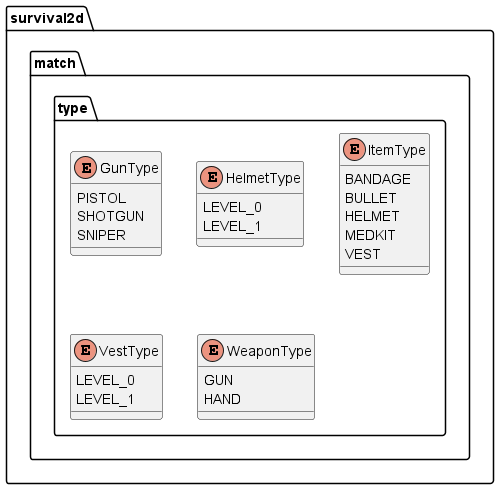
\includegraphics[width=0.6\textwidth]{Img/uml/type.png}
    \caption{Diagram của các enum}
    Các enum này chứa thông số để config cho game.
  \end{figure}

  \begin{sidewaysfigure}
    \centering
    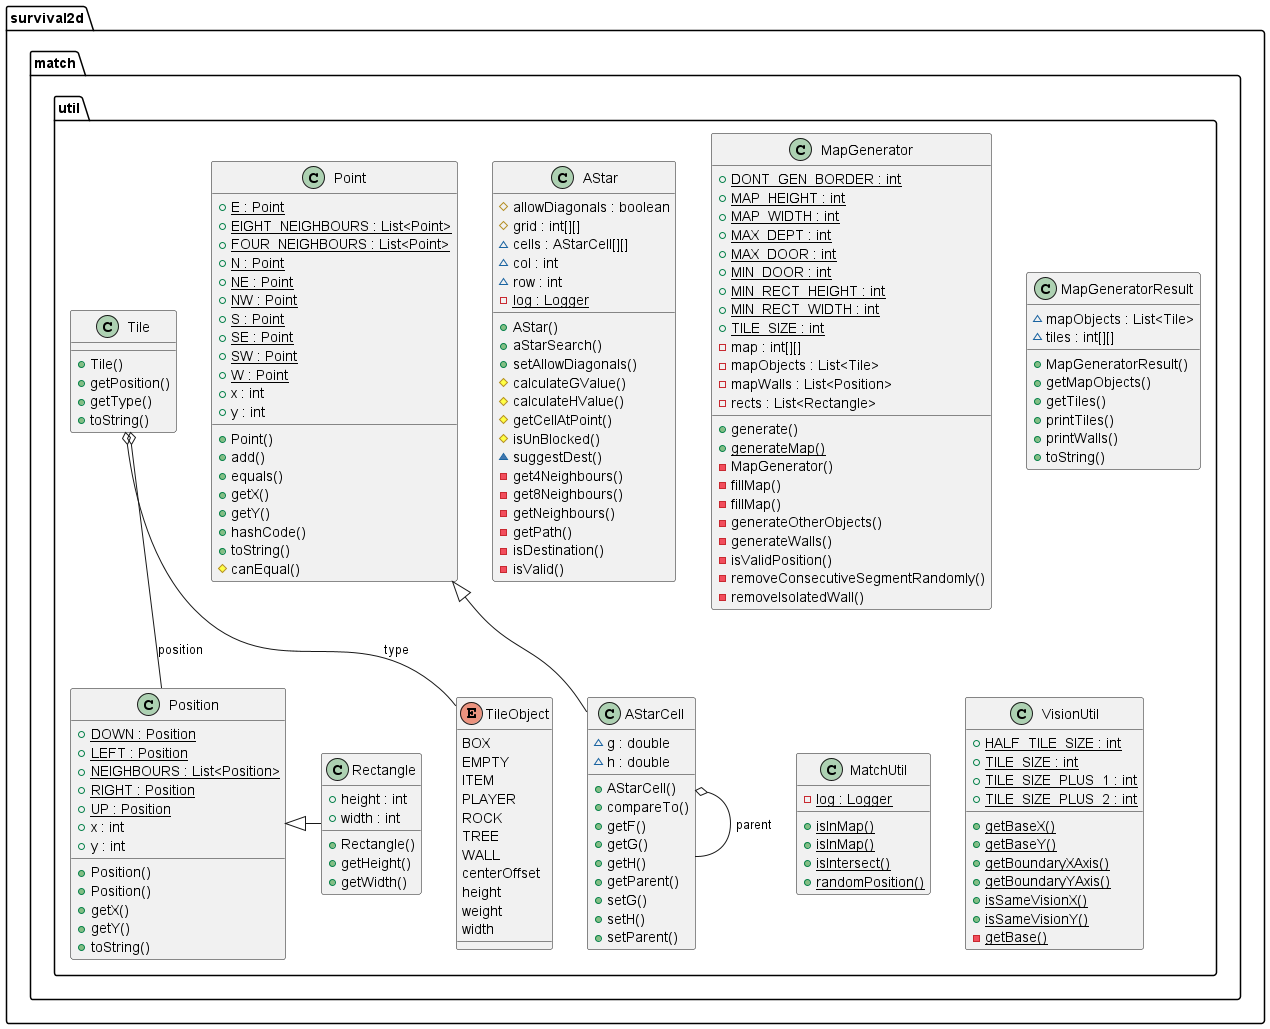
\includegraphics[width=0.8\textwidth]{Img/uml/util.png}
    \caption{Diagram của các class hỗ trợ}
    Các class này thực hiện những việc phổ biến, sử dụng lại nhiều trong game.
  \end{sidewaysfigure}

  \begin{figure}[H]
    \centering
    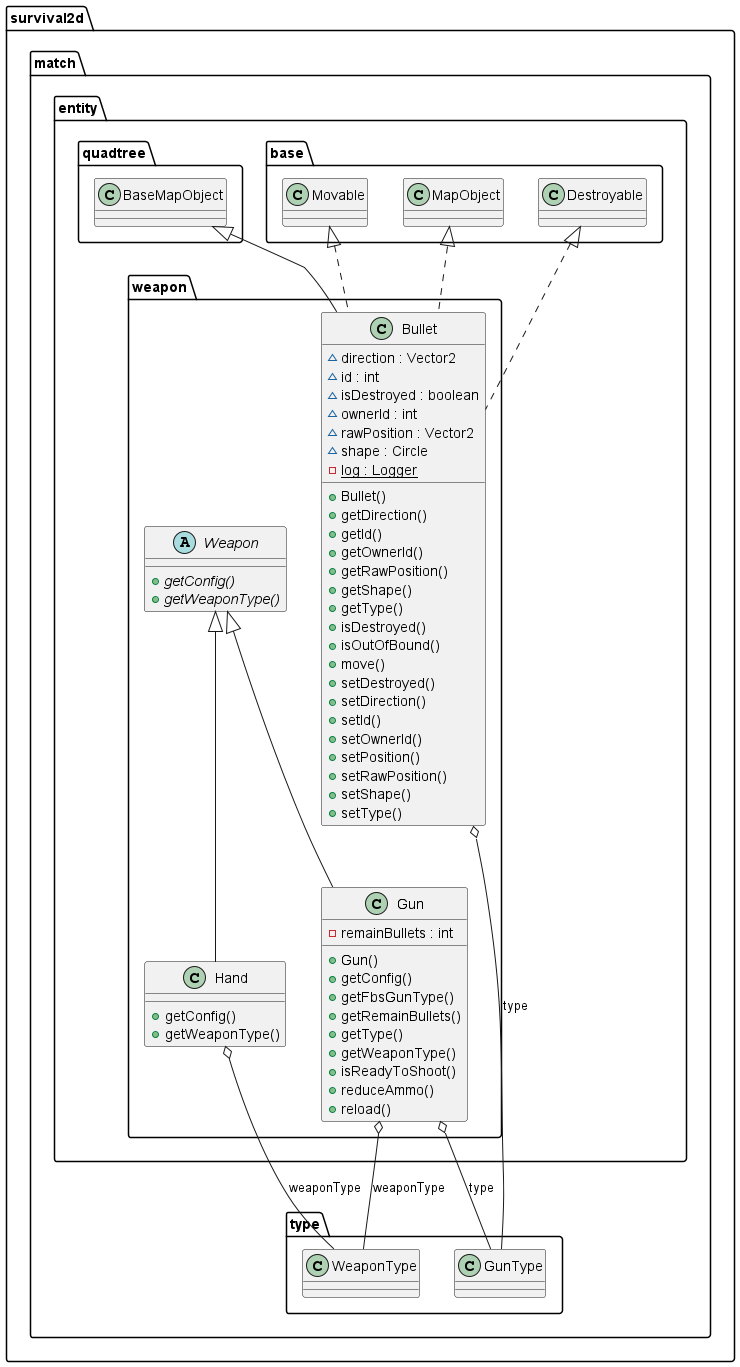
\includegraphics[width=\textwidth,height=0.9\textheight,keepaspectratio]{Img/uml/weapon.png}
    \caption{Diagram của các class vũ khí trong \textbf{Survival2D}}
    Các class này cho biết trạng thái của vũ khí và cho phép lấy chỉ số của vũ khí trong game dễ dàng hơn.
  \end{figure}

  \subsubsection{Quản lý các object trong map}

  \paragraph{Vấn đề}\mbox{}
  
  Trong một map lớn, rất nhiều objects, và thời gian cập nhật của mỗi vòng lặp logic cũng rất nhanh, nên khi các object tương tác với nhau, nếu phải duyệt qua toàn bộ các objects khác thì chi phí vòng lặp tăng lên nhiều lần. Ví dụ để khi đạn di chuyển, nếu ta phải duyệt qua toàn bộ map objects và players để kiểm tra va chạm và tính toán sát thương thì sẽ tốn chi phí $n^2$, với lượng map objects lên đến hàng nghìn của \textbf{Survival2D}, và không chỉ mỗi việc kiểm tra va chạm của đạn, còn có va chạm của player để cản player di chuyển,... thì đây là một chi phí lớn. Vì vậy cần có giải pháp để có thể tìm ra các vật thể xung quanh một object nhanh hơn, đảm bảo vòng lặp xử lý logic của game xử lý nhanh, đáp ứng được yêu cầu realtime.
  
  Và đó lí do nhóm áp dụng mẫu thiết kế \textit{Spatial Partition} (tạm dịch \textit{"Phân vùng không gian"}) để quản lý các object.

  \paragraph{Giải pháp}\mbox{}

   Ý tưởng của mẫu thiết kế \textit{Phân vùng không gian} cũng giống với Binary search trên mảng 1 chiều. Đơn giản hóa bài toán "Tìm các vật thể xung quanh bán kính \textit{x} của một vị trí cho trước trên một bản đồ 2D" thành "Tìm các số có khoảng cách so với một số cho trước $\le$ \textit{x} trong một mảng 1 chiều". Để giải quyết bài toán này, nếu đảm bảo các phần tử trong mảng đã được sắp xếp, ta có thể dùng Binary search để tìm các số thích hợp, thay vì phải duyệt qua toàn bộ mảng.

   Mẫu thiết kế Phân vùng không gian cũng giống vậy, nhưng mở rộng ra cho không gian 2 chiều. Nó cho phép xác định nhanh các đối tượng xung quanh một vị trí cho trước; bằng cách sử dụng cấu trúc dữ liệu được sắp xếp theo vị trí 2 chiều của chúng. Nhờ vậy khi thực hiện một thao tác như kiểm tra va chạm ở trên, không cần phải kiểm tra vị trí của \textit{mọi} đối tượng so với vị trí của đối tượng cần xét va chạm.
   
   Cấu trúc dữ liệu có thể được sử dụng để lưu trữ các đối tượng chuyển động và hoặc đứng yên; với các đối tượng chuyển động, chúng sẽ được gỡ ra và chèn lại mỗi khi vị trí của chúng thay đổi. Trong \textbf{Survival2D}, nhóm sử dụng Quadtree, cấu trúc này sẽ giảm độ phức tạp về thời gian của việc tìm kiếm các đối tượng trong một phạm vi nhất định từ $O(n^2)$ còn $O(n*log(n))$, giảm đáng kể các tính toán cần thiết trong trường hợp có số lượng lớn đối tượng.

   Hình \ref{spatial_pattern_quadtree} biểu diễn mẫu thiết kế Phân vùng không gian sử dụng cấu trúc dữ liệu QuadTree, map sẽ được chia thành nhiều vùng nhỏ cho đến khi mỗi vùng chỉ chứa tối đa 2 objects.

   \begin{figure}[H]
      \centering
      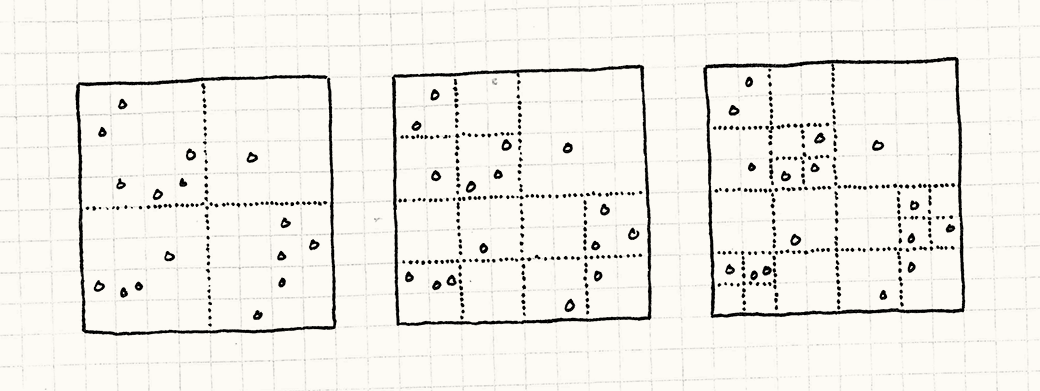
\includegraphics[width=\textwidth]{Img/map/spatial-partition-quadtree.png}
      \caption{Mẫu thiết kế Phân vùng không gian sử dụng cấu trúc dữ liệu QuadTree\protect\footnotemark}
      \label{spatial_pattern_quadtree}
  \end{figure}
  \footnotetext{Nguồn: \url{https://gameprogrammingpatterns.com/spatial-partition.html}}
  
  \subsubsection{Sinh map ngẫu nhiên}
  Để có được một cấu trúc map (map config) phù hợp, thiết kế thủ công sẽ giúp ta tinh chỉnh chính xác được những gì ta muốn trên một map để map cân bằng và thú vị. Tuy nhiên, việc này sẽ tốn rất nhiều thời gian, nên sẽ khó tạo ra được nhiều map. Nếu game chỉ có một hoặc hai map lặp đi lặp lại thì người chơi sẽ cảm thấy nhàm chán, do đó một thuật toán sinh map ngẫu nhiên sẽ được xây dựng trong game để đáp ứng được sự đa dạng về trải nghiệm của người chơi.
  
  Thuật toán sẽ sinh ra một config chứa thông tin của map gồm kích thước, hình dạng (dựa theo từng tile của tilemaps), vị trí các objects trên map,... sau đó game sẽ đọc config, tạo logic map và render map.

  \paragraph{Thuật toán tạo bản đồ}\mbox{}

  Chia map 10000x10000 pixels ban đầu thành nhiều ô, mỗi ô có kích thước 100x100 pixels. Map ban đầu sẽ trở thành một map 100x100 ô, tổng quát là một hình chữ nhật có chiều dài $W$, chiều rộng $H$. Để đảm bảo những "khu vực" được ngăn cách bởi tường đủ lớn, ta sẽ gọi khoảng chiều dài, chiều rộng nhỏ nhất này là $minSpace$. Sau đó chọn một giá trị $v$ sao cho $minSpace \le v \le W$ và một giá trị $h$ sao cho $minSpace \le h \le H$. Sau đó thêm một hàng tường có $x = v$ hoặc $y = h$. Ta được 4 đoạn tường nhỏ chia cắt map. Để đảm bảo map liên thông với nhau, ta sẽ "đục" 3 trên 4 tường này để tạo lối đi. Ngoài ra để đảm bảo dễ dàng di chuyển giữa các vùng, ta cũng tiến hành đục nếu tường quá dài (có độ dài lớn hơn $L$ cho trước). Và đệ quy hàm này cho 4 hình chữ nhật mới (sau khi bị chia cắt bởi 2 đường kẻ); cho đến khi $W, H < minSpace/2$ (để đảm bảo khu vực mới tạo ra không quá nhỏ như đã nói ở trên).

  Sau đó ta sẽ tạo ra những vật cản khác trên map cho từng "khu vực". Để đảm bảo vật cản mới sinh ra không bịt kín lối đi, ta sẽ gen vật cản cách tường một khoảng là $offset$. Các vật cản này được tạo ra theo tỉ lệ trong config cho trước. Với mỗi "khu vực" ta cũng chọn ra một ô trống để đánh dấu có thể cho người chơi xuất hiện tại ô này; để sau khi gen map, ta có một list những vị trí có thể cho người chơi xuất hiện. Bằng cách này, có thể đảm bảo mỗi player ban đầu sẽ có được một khu vực an toàn, nhưng vẫn có vật phẩm, đảm bảo cân bằng game. Hình \ref{genmap} mô tả cho thuật toán này.
  
  \begin{figure}[H]
  \centering
  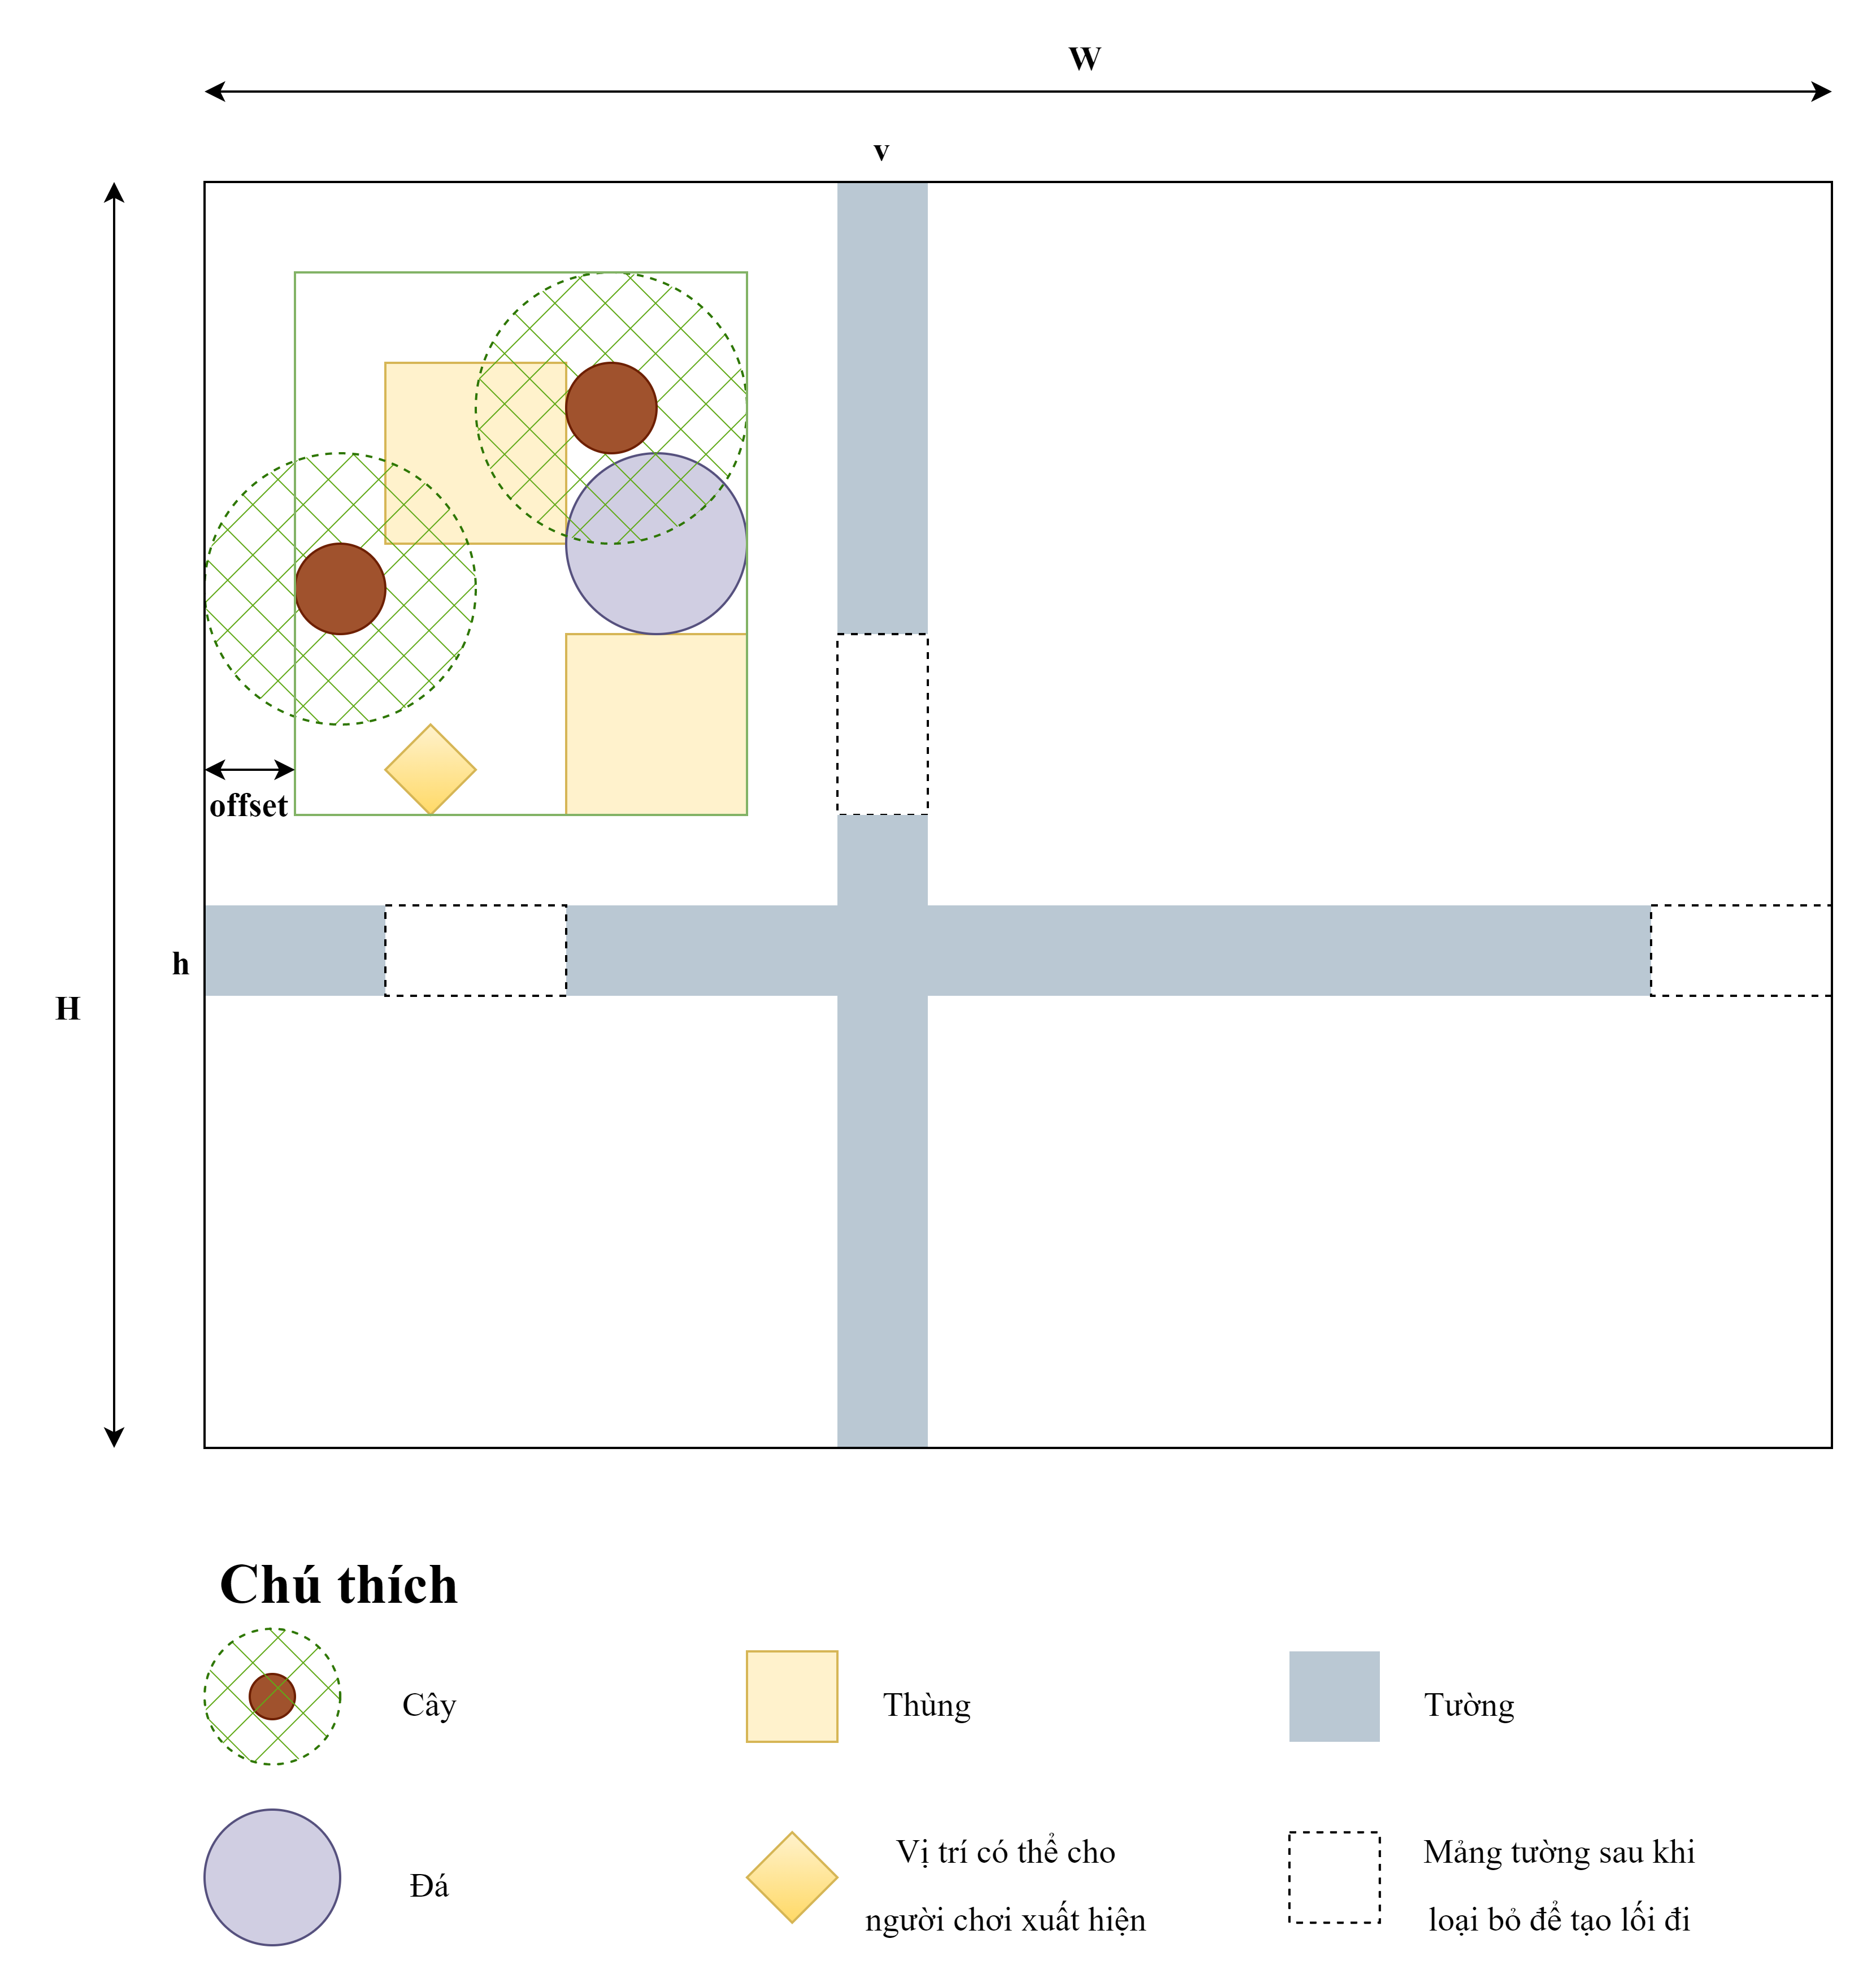
\includegraphics[width=\textwidth]{Img/map/genmap.png}
  \caption{Mô tả thuật toán tạo bản đồ}
  \label{genmap}
  \end{figure}
  
  Sử dụng thuật toán này cho map ban đầu, ta có thể đạt được kết quả là map như trong hình \ref{mapoverview}.

  \begin{figure}[H]
  \centering
  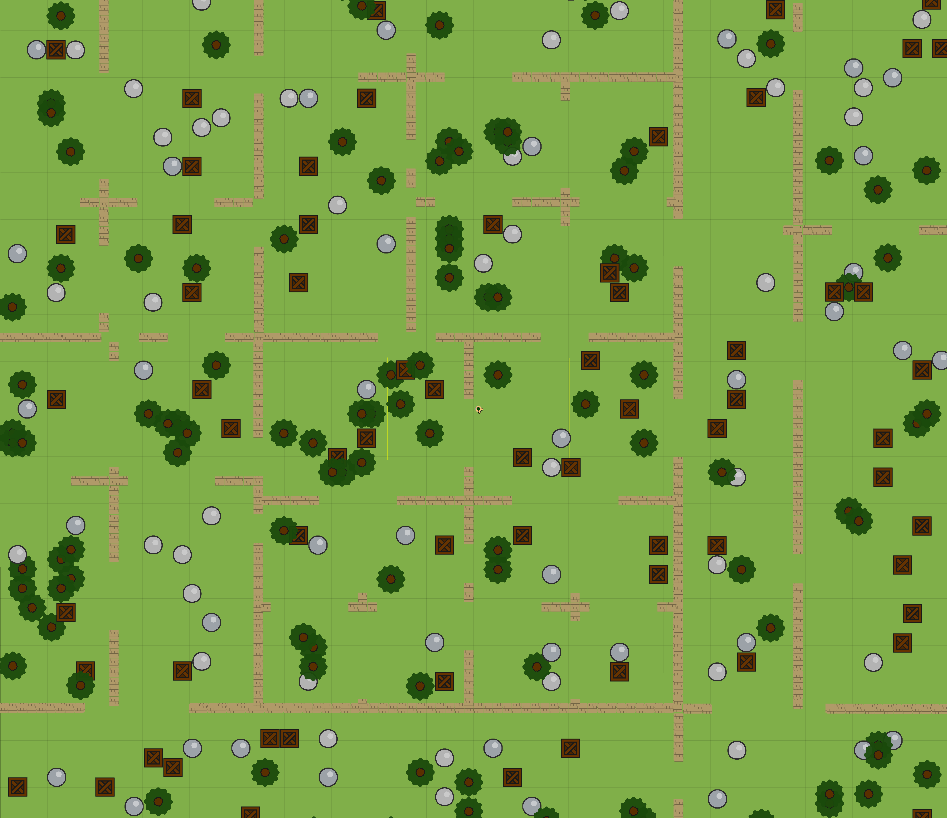
\includegraphics[width=\textwidth]{Img/map/overview.png}
  \caption{Tổng thể map được tạo ra bởi thuật toán tạo bản đồ}
  \label{mapoverview}
  \end{figure}

  \begin{it}
    \paragraph{Chú thích}
    \begin{itemize}
      \item Các đường màu vàng cam, liên kết với nhau là tường.
      \item Các hình tròn màu xanh lá có viền răng cưa, bao quanh một hình tròn màu nâu là cây (phần màu nâu là gốc cây, phần màu xanh là tán cây).
      \item Các hình tròn màu xám là đá.
      \item Các hình vuông có dấu chéo là các thùng gỗ có chứa item.
    \end{itemize}
  \end{it}
  
  \subsection{Thiết kế mô hình client-server}
  \subsubsection{Thiết kế cơ bản}
  Hầu hết các trò chơi trực tuyến ngày nay đều được thiết kế theo mô hình client-server. Trong thiết kế này, có một server duy nhất chịu trách nhiệm xử lý các logic chính của game. Server này sau đó được kết nối đến một hoặc nhiều client. Các client này có nhiệm vụ thu thập các input từ người chơi, sau đó gửi đến server để xử lý, server sử dụng các input đó để cập nhật lại các thông số của các vật thể trong trò chơi (như vị trí, trạng thái, ...) rồi gửi lại các cập nhật đó cho client hiển thị.
  Mỗi client và server đều chạy các vòng game loop của riêng mình và xử lý các công việc khác nhau trong vòng lặp đó.
  
  Đối với client, vòng lặp sẽ được chạy mỗi frame và làm các công việc như sau:
  \begin{enumerate}
      \item Thu thập các input của người chơi.
      \item Đóng gói và gửi các input của người chơi cùng với frametime.
      \item Đọc các gói tin trả về từ server và cập nhật lại thông tin của các vật thể cần hiển thị.
      \item Render game
  \end{enumerate}
  
  Đối với server, vòng lặp sẽ có dạng như sau:
  \begin{enumerate}
      \item Đọc các input từ client.
      \item Xử lý các input từ client.
      \item Mô phỏng game sử dụng frame time.
      \item Tạo các gói cập nhật của game tương ứng với từng client và gửi đi.
  \end{enumerate}
  
  Với cấu trúc client-server đơn giản như trên, về cơ bản hệ thống sẽ hoạt động như sau: Đầu tiên client tạo và gửi các input từ người dùng đến cho server, server sau đó xử lý và cập nhật lại trạng thái tất cả các vật thể cho client để client hiển thị.

  \begin{figure}[H]
  \centering
  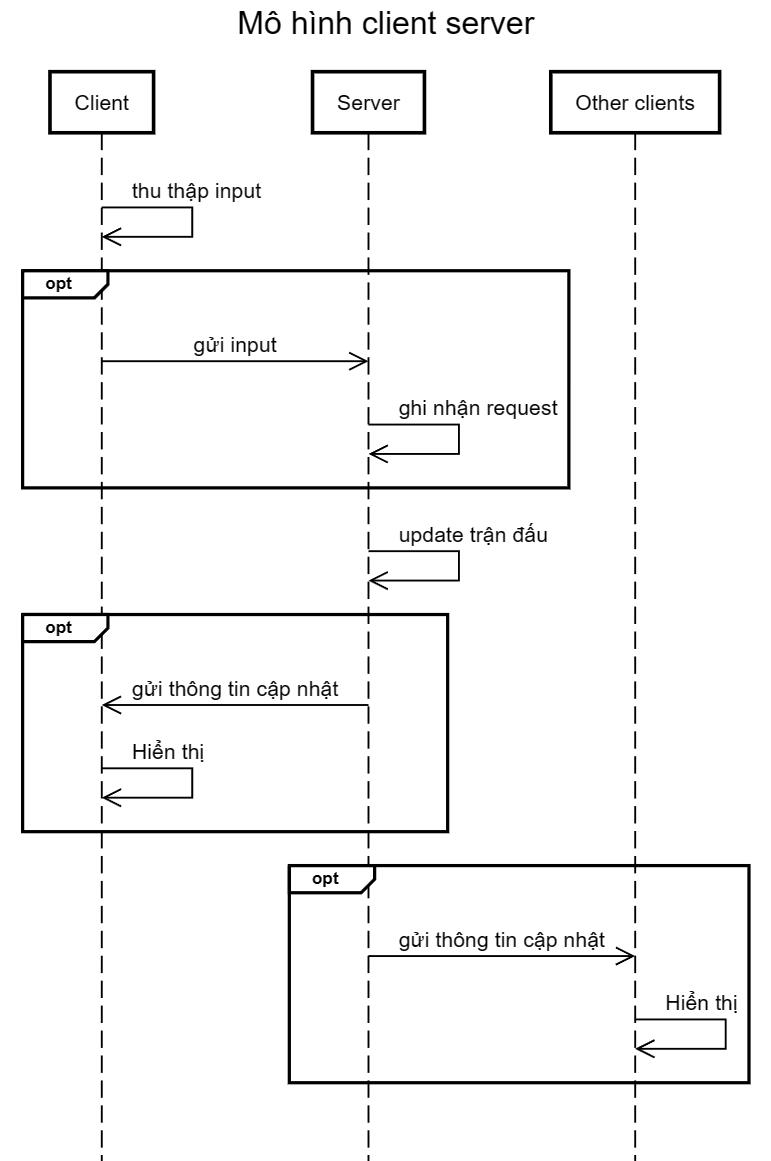
\includegraphics[width=\textwidth,height=0.9\textheight,keepaspectratio]{Img/clientserver/Client-Server.png}
  \caption{Minh hoạ mô hình client-server}
  \end{figure}
  
  Thiết kế trên tuy khá đơn giản và dễ hiện thực nhưng lại gặp nhiều vấn đề khi triển khai trên môi trường mạng. Vấn đề lớn nhất chính là sự ảnh hưởng của độ trễ khi gửi gói tin đến trải nghiệm chơi game của người chơi. Giả sử một gói tin input của người chơi mất một khoảng thời gian 50ms để đi từ client đến server, đợi server xử lý rồi trả ngược kết quả về cho client, và gói tin trả về này cũng mất 50ms mới đến nơi, thì tất cả các hành động của người chơi đều sẽ phải đợi 100ms sau mới thấy được kết quả của hành động đó trên màn hình. Nếu trong một trò chơi một người, ta có thể tạm chấp nhận độ trễ đó, nhưng trong một trò chơi nhiều người với diễn biến nhanh và chỉ cho phép sai lệch tối đa vài chục mili giây, ta cần có các kỹ thuật để hạn chế sự ảnh hưởng của vấn đề độ trễ này đến trải nghiệm người chơi.
  
  \subsubsection{Kỹ thuật dự đoán phía client}
  Một kỹ thuật để hạn chế ảnh hưởng của độ trễ mạng là client thay vì chỉ thực hiện các chức năng đơn giản là thu thập input và render theo kết quả trả về từ server thì sẽ tự thực hiện hành động của người chơi ngay sau khi nhận được input một cách địa phương trên client đó mà không cần đợi kết quả trả về từ server.
  
  Điều này không có nghĩa là mỗi client sẽ chạy một logic khác nhau mà server vẫn sẽ xử lý input của người chơi như bình thường và sau đó khi client nhận được gói tin kết quả, client sẽ sửa lại trạng thái của các object trong game cho đúng với kết quả trong gói tin đó. Điểm trừ của kỹ thuật này là khi client sửa lại trạng thái các vật thể theo kết quả, có thể sẽ gây ra một sự "giật" nhẹ; nếu việc này xảy ra quá thường xuyên sẽ ảnh hưởng đến trải nghiệm game của người chơi.
  
  \subsection{Thiết kế người chơi máy (bot)}
  \subsubsection{Thuật toán tìm đường đi cho bot}
  Thuật toán tìm đường đi ngắn nhất cần được áp dụng cho bot khi bot cần di chuyển đến khu vực an toàn, đi nhặt trang bị hay chạy trốn một cách nhanh nhất. Tuy nhiên ở trường hợp tìm địch và chiến đấu, đường đi của bot cần phải linh hoạt và tự nhiên hơn (đi vòng, né tránh,...), do đó giải thuật cần được cải tiến, hoặc thậm chí sẽ phải dùng thêm giải thuật khác để đáp ứng điều này.

  Trước tiên, giải pháp mà \textbf{Survival2D} sử dụng là giải thuật A*. Trong khoa học máy tính, A* là thuật toán tìm kiếm trong đồ thị và là một thuật toán tìm kiếm theo lựa chọn tốt nhất (best-first search). Thuật toán này tìm một đường đi từ một nút khởi đầu đến một nút đích cho trước (hoặc đến một nút thỏa mãn một điều kiện đích). Thuật toán này sử dụng một hàm heuristic để đánh giá và xếp loại từng nút theo ước lượng về tuyến đường tốt nhất đi qua nút đó.
  \begin{figure}[H]
      \centering
      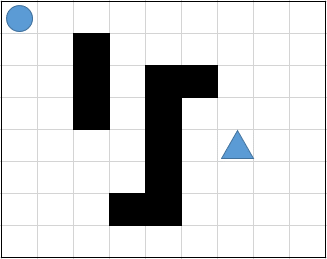
\includegraphics[width=0.5\textwidth]{Img/AI/A_Star_image1.png}
      \caption{Minh hoạ bài toán tìm đường\cite{a_star}}
  \end{figure}
  \begin{figure}[H]
      \centering
      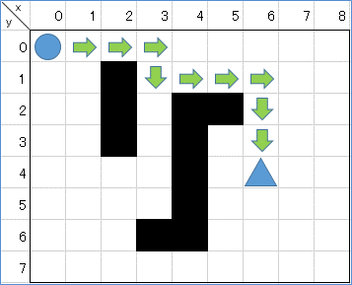
\includegraphics[width=0.5\textwidth]{Img/AI/A_Star_image2.png}
      \caption{Minh hoạ kết quả tìm đường áp dụng A*\cite{a_star}}
  \end{figure}

  \paragraph{Mô tả thuật toán}\mbox{}

  A* lưu giữ một tập các lời giải chưa hoàn chỉnh trong một hàng đợi ưu tiên (priority queue), nghĩa là các đường đi qua đồ thị, bắt đầu từ nút xuất phát. Thứ tự ưu tiên gán cho một đường đi \(x\) được quyết định bởi hàm
  \(f(x) = g(x) + h(x)\), trong đó:
  \begin{itemize}
      \item \(g(x)\): là chi phí của đường đi cho đến thời điểm hiện tại, nghĩa là tổng trọng số của các cạnh đã đi qua
      \item \(h(x)\): là hàm heuristic ước lượng về chi phí nhỏ nhất để đến đích nếu đi qua \(x\)
  \end{itemize}
  
  \subsubsection{Xây dựng cây hành vi (behavior tree) quản lý hành vi cho bot}
  Cây hành vi (behavior tree) là một mô hình toán học được sử dụng phổ biến trong các lĩnh vực như khoa học máy tính (computer science), người máy (robotics), hệ thống điều khiển (control systems) và đặc biệt là trong công nghiệp game (video game industry). Behavior tree mô tả việc chuyển đổi giữa một tập hợp hữu hạn các nhiệm vụ theo kiểu module, mỗi module là một nhiệm vụ phức tạp được tạo thành từ các nhiệm vụ nhỏ đơn giản hơn, và cái hay của behavior tree là không cần biết các nhiệm vụ nhỏ đó được hiện thực thế nào.
  
  So sánh với một mô hình khác là máy trạng thái (state machine)\cite{finite_state_machine} phổ biến không kém trong lĩnh vực khoa học máy tính và cũng có thể dùng để quản lý trạng thái cho bot, behavior tree cho thấy sự trực quan hơn, thân thiện, dễ hiểu hơn với đời sống thực khi quản lý hành vi bằng các module nhiệm vụ, quyết định hành động thực tế của nhân vật xuyên suốt game thay vì quản lý trạng thái của chúng. Không dừng lại ở đó, behavior tree thực sự mạnh khi có khả năng thực thi nhiều nhiệm vụ cùng lúc bằng cách thêm các nhiệm vụ song song, trong khi state machine chỉ có thể có một trạng thái trong một thời điểm. Bên cạnh đó tính linh hoạt và khả năng mở rộng cũng tốt hơn state machine nhờ vào cấu trúc cây. Các điểm mạnh kể trên cho thấy behavior tree cực kỳ phù hợp trong việc thiết kế bot dành cho cộng đồng phát triển game nói chung và cho \textbf{Survival2D} nói riêng.\cite{behavior_tree_wiki}

  \paragraph{Khái quát về ý tưởng của behavior tree}\mbox{}

  Như đã nêu trên, behavior tree có cấu trúc cây và là một cây gồm các nút con phân tầng, kiểm soát chuỗi các hành vi của bot. Các nút trong hay còn gọi là các cây con của behavior tree đại diện cho một nhóm các nhiệm vụ, nút càng sâu thì nhiệm vụ càng rõ ràng. Duyệt đến tầng sâu nhất ta sẽ gặp các nút lá, chính là nhiệm vụ thực sự mà bot cần phải thực hiện. Nói dễ hiểu hơn khi xét cây từ dưới lên là: các nút lá là các lệnh thực điều khiển hành vi, các nút trong "gộp nhóm" các nút lá lại theo từng nhóm nhiệm vụ. Hình \ref{fig:simple_bt_node_example} và \ref{fig:combind_bt_node_example} là một ví dụ về việc "gộp nhóm" các nhóm nhiệm vụ trong cấu trúc của behavior tree.
  \begin{figure}[H]
      \centering
      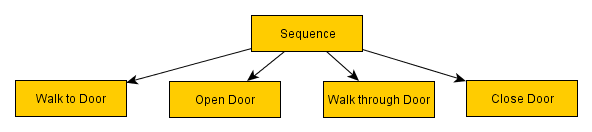
\includegraphics[width=0.75\textwidth]{Img/AI/simple-node-of-behavior-tree-1.png}
      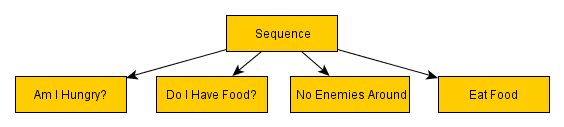
\includegraphics[width=0.75\textwidth]{Img/AI/simple-node-of-behavior-tree-2.png}
      \caption{Minh hoạ các nhiệm vụ đơn giản của behavior tree\cite{bib17}}
      \label{fig:simple_bt_node_example}
  \end{figure}
  \begin{figure}[H]
      \centering
      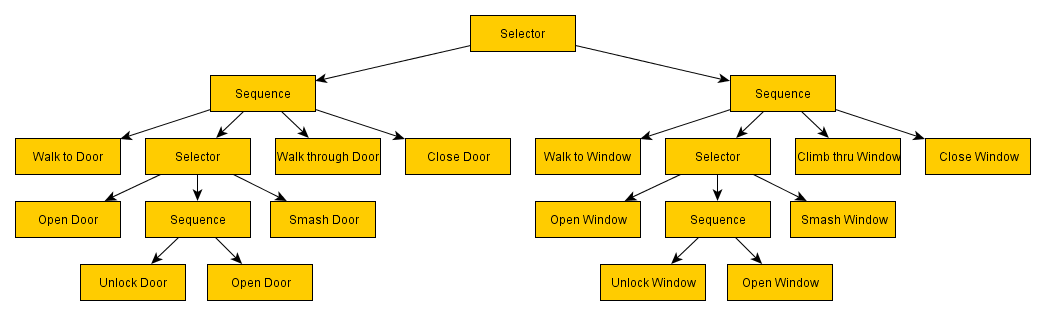
\includegraphics[width=1\textwidth]{Img/AI/complex-node-of-behavior-tree.png}
      \caption{Minh hoạ một nhiệm vụ phức tạp hơn của behavior tree\cite{bib17}}
      \label{fig:combind_bt_node_example}
  \end{figure}

  \begin{figure}[H]
      \centering
      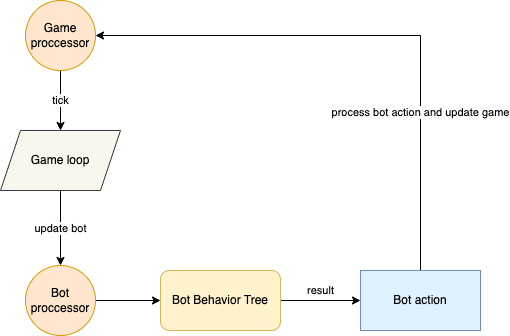
\includegraphics[width=0.7\textwidth]{Img/AI/bot_tick.png}
      \caption{Cách hoạt động của bot sử dụng behavior tree}
  \end{figure}

  Luồng thực thi của behavior tree cũng rất đơn giản. Ở mỗi thời điểm trong game (tick), ta duyệt cây tiền thứ tự (preorder), thực thi nút lá và trả về kết quả. Kết quả từ các nút con sẽ quyết định kết quả cho cha của nó theo một số quy luật cụ thể, từ đó quyết định nhiệm vụ tiếp theo sau được duyệt đến và thực thi hay là bị cắt tỉa và chuyển sang nhiệm vụ khác. Cứ thế cho đến nhiệm vụ cuối cùng theo thứ tự duyệt cây. Tập các nút lá mà ta duyệt đến được chính là các nhiệm vụ mà bot thực thi trong tick đó.

  Các kết quả mà một nút có thể trả về bao gồm:
  \begin{itemize}
      \item SUCCESS - phản ánh nhiệm vụ thành công.
      \item FAILURE - phản ánh nhiệm vụ thất bại.
      \item RUNNING - phản ánh nhiệm vụ đang trong quá trình thực thi, chưa có kết quả sau cùng.
  \end{itemize}
  \par{}

  \paragraph{Behavior tree sử dụng cho \textbf{Survival2D}}\mbox{}

  Có thể thấy quy luật quyết định kết quả của một nút trong là rất quan trọng.
  Áp dụng vào đề tài, behavior tree của \textbf{Survival2D} sử dụng những loại nút trong cơ bản sau đây:
  \begin{itemize}
      \item \textit{Sequence}
      
      Thực thi các nút con theo thứ tự, FAILURE nếu có bất cứ nút con nào FAILURE.
      
      Nút Sequence thường dùng trong các trường hợp nhiệm vụ có nhiều bước, cần phải hoàn thành hết các bước, hay đơn giản có thể dùng để kiểm tra điều kiện trước khi thực hiện nhiệm vụ.
      \begin{figure}[H]
          \centering
          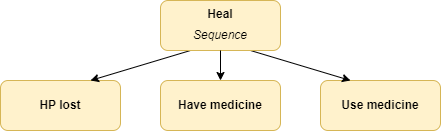
\includegraphics[width=0.75\textwidth]{Img/AI/heal.png}
          \caption{Ví dụ về nút Sequence trong \textbf{Survival2D}}
          \label{heal_node}
          Bot sẽ thực hiện các nhiệm vụ kiểm tra có bị mất máu hay không, sau đó kiểm tra có thuốc hồi máu hay không, cuối cùng là dùng thuốc để hồi máu.
      \end{figure}
      \item \textit{Selector}
      
      Thực thi các nút con theo thứ tự, SUCCESS nếu có bất cứ nút con nào SUCCESS.
      
      Nút Selector thường dùng trong các trường nhiệm vụ có nhiều cách để hoàn thành, và có thể dùng để kiểm tra điều kiện trước khi thực hiện nhiệm vụ (có thể xem Selector là đối nghịch với Sequence, Selector là phép OR và Sequence là phép AND).
      \begin{figure}[H]
          \centering
          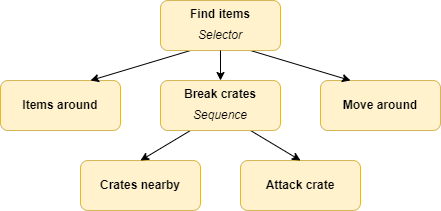
\includegraphics[width=0.75\textwidth]{Img/AI/find-items.png}
          \caption{Ví dụ về nút Selector trong \textbf{Survival2D}}
          Có nhiều cách để tìm kiếm một vật phẩm, bao gồm kiểm tra vật phẩm xung quanh, đập thùng tìm và di chuyển đến chỗ khác nếu cả hai nhiệm vụ trước đều FAILURE.
      \end{figure}
      
      \item \textit{Inverter}
      
      Thực thi nút con (Inverter chỉ có một con) sau đó trả về kết quả ngược lại với con của nó.
      
      Nút Inverter cơ bản thường dùng trong kiểm tra điều kiện, có thể tận dụng những nút có sẵn rồi đảo kết quả lại, giảm số lượng nút cần phải hiện thực.
      \begin{figure}[H]
          \centering
          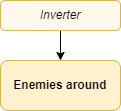
\includegraphics[width=0.2\textwidth]{Img/AI/inverter.png}
          \caption{Ví dụ về nút Inverter trong \textbf{Survival2D}}
          Đảo nghịch kết quả của nhiệm vụ kiểm tra địch xung quanh thay vì định nghĩa nhiệm vụ mới.
      \end{figure}
      \item \textit{Succeeder}
      
      Thực thi nút con (Succeeder chỉ có một con) sau đó luôn trả về SUCCESS.
      
      Nút Succeeder dùng cho những nhiệm vụ không bắt buộc, giúp chúng được thực thi nếu có thể và không quan tâm về kết quả có thành công hay không, không làm ảnh hưởng đến luồng thực thi các nhiệm vụ tiếp theo.
      \begin{figure}[H]
          \centering
          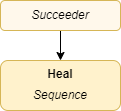
\includegraphics[width=0.2\textwidth]{Img/AI/succeeder.png}
          \caption{Ví dụ về nút Succeeder trong \textbf{Survival2D}}
          Hồi máu là một hành vi có thể xảy ra song song với nhiều hành vi khác (không để phí thời gian và đảm bảo lượng máu là tốt nhất có thể), vì vậy Succeeder giúp nhiệm vụ hồi máu được thực thi cùng với những nhiệm vụ khác.
      \end{figure}
      \item \textit{Repeat Until Success}
      
      Ngoài ra còn một loại kết quả nữa là RUNNING. Khi một nút con trả về RUNNING, kết quả của nút cha cũng sẽ là RUNNING và nhiệm vụ đó được hiểu là đang thực thi, vào tick tiếp theo nó sẽ được tiếp tục.
      
      Repeat Until Success thực thi nút con (chỉ có một con) lặp lại ở mỗi tick cho đến khi nút con SUCCESS, nếu nút con FAILURE nó sẽ trả về RUNNING. Ta cũng có thể biến đổi điều kiện một chút để có thêm giới hạn số lần lặp, dành cho các nhiệm vụ chỉ cho phép thử thực hiện lại trong một khoảng thời gian nhất định.
     \begin{figure}[H]
          \centering
          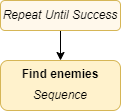
\includegraphics[width=0.2\textwidth]{Img/AI/repeat-until-success.png}
          \caption{Ví dụ về nút Repeat Until Success trong \textbf{Survival2D}}
          Trong khi đang ở trạng thái tấn công, bot sẽ đi tìm địch nếu không thấy địch, và sẽ tìm đến khi thấy địch mới chuyển sang hành động tấn công địch.
      \end{figure}
  \end{itemize}
  Từ những nút cơ bản kể trên, cấu trúc behavior tree rút gọn quản lý hành vi của bot trong \textbf{Survival2D} được xây dựng như sau:
  \begin{figure}[H]
      \centering
      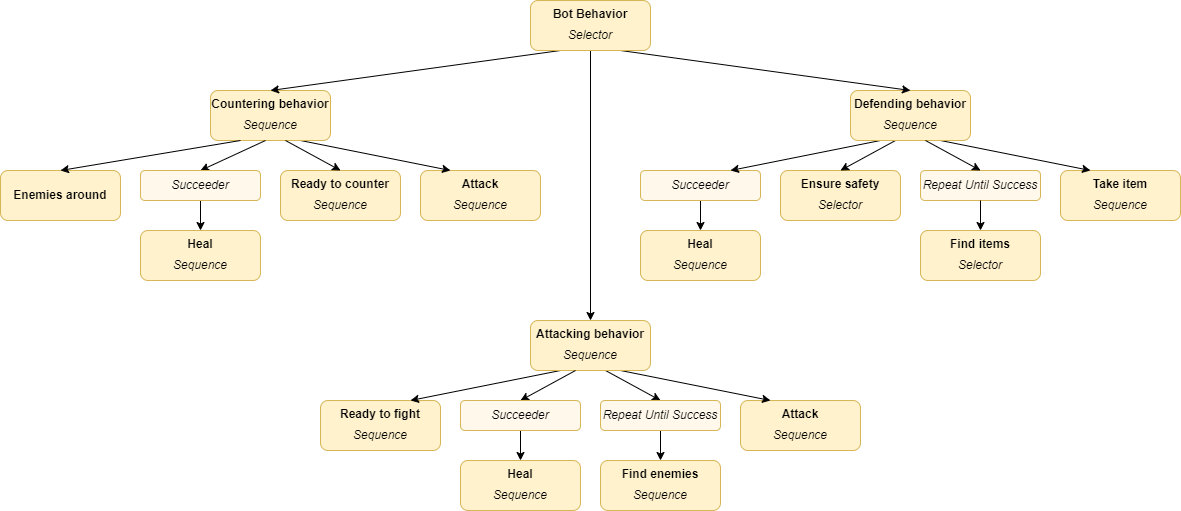
\includegraphics[width=1\textwidth]{Img/AI/bot-behavior.png}
      \caption{Behavior tree rút gọn của \textbf{Survival2D}}
  \end{figure}
  Sau mỗi tick, bot sẽ mang một trạng thái là phản công, tấn công hoặc phòng thủ, tuỳ vào nhóm hành vi tương ứng nào sẽ SUCCESS. Sở dĩ 3 trạng thái này có thể sắp xếp theo một thứ tự khác, tuy nhiên cách hiện thực các nhiệm vụ con sẽ phải thay đổi đôi chút để vừa đảm logic vừa không làm cấu trúc cây trở nên quá rối.

  Theo cách hiện thực trên, nhóm hành vi phản công được duyệt đến đầu tiên. Khi duyệt qua nhóm này, hành vi đầu tiên mà bot thực hiện là kiểm tra có địch xung quanh hay không, nếu có thì sẽ tiếp tục thực hiện nhiệm vụ tiếp theo để phản công bao gồm hồi máu, kiểm tra có đủ trang bị để phản công hay không, và sau đó tấn công kẻ địch. Nếu không có địch xung quanh, hoặc có nhưng lại không đủ trang bị, cây sẽ duyệt tiếp sang nhóm hành vi tấn công.

  Ở nhóm hành vi tấn công, đầu tiên bot kiểm tra có trang bị, máu đã sẵn sàng chiến đấu hay chưa, hồi máu nếu có thể, tìm kiếm địch và tấn công tiêu diệt địch sau khi tìm thấy. Khi không đủ sẵn sàng để tấn công nữa, cây duyệt tiếp sang nhóm hành vi cuối là nhóm phòng thủ.

  Khi chuyển sang phòng thủ, đầu tiên dĩ nhiên lại là hồi máu nếu có thể, sau thực hiện nhiệm vụ đảm bảo an toàn cho bản thân. Khi đã an toàn rồi, bot sẽ đi tìm vật phẩm để tăng cường trang bị cũng như có thêm thuốc để hồi máu, và khi đã đủ điều kiện sẵn sàng quay lại chiến đấu, bot hoàn toàn có thể quay lại nhóm hành vi phản công hoặc chủ động tấn công ở tick tiếp theo.

  Ngoài nút nhiệm vụ hồi máu (Heal) và nhiệm vụ tìm vật phẩm (Find items) đã được mô tả trong ví dụ về Sequence và Selector, cấu trúc cây trên còn có các nút nhiệm vụ khác đã được rút gọn, chưa mô tả rõ là: sẵn sàng phản công (Ready to counter), sẵn sàng chiến đấu (Ready to fight), tìm địch (Find Enemies), tấn công (Attack), bảo đảm an toàn (Ensure safety) và nhặt vật phẩm (Take item).

  \begin{figure}[H]
      \centering
      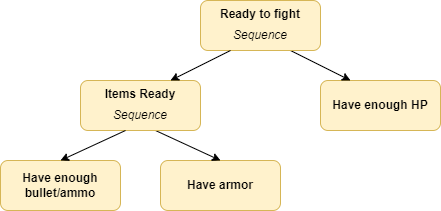
\includegraphics[width=0.75\textwidth]{Img/AI/ready-to-fight.png}
      \caption{Thiết kế của nhiệm vụ kiểm tra sẵn sàng chiến đấu}
  \end{figure}
  Bot trong \textbf{Survival2D} kiểm tra tình trạng của chính nó có sẵn sàng chiến đấu hay không bằng cách: kiểm tra vũ khí trang bị đầy đủ bao gồm đầy đủ các loại đạn, giáp, và kiểm tra máu có ở mức an toàn chưa.

  \begin{figure}[H]
      \centering
      \includegraphics[width=0.25\textwidth]{Img/AI/ready-to-counter.png}
      \caption{Thiết kế của nhiệm vụ kiểm tra sẵn sàng phản công}
  \end{figure}
  Điều kiện sẵn sàng phản công thì ít hơn so với sẵn sàng chiến đấu vì lúc đó có địch ở gần nên tình hình cấp bách hơn, chỉ cần có đủ đạn là đã phản công được.

  \begin{figure}[H]
      \centering
      \includegraphics[width=0.5\textwidth]{Img/AI/find-enemies.png}
      \caption{Thiết kế của nhiệm vụ tìm địch}
  \end{figure}
  Vì không biết được địch đang ở những vị trí nào trên map nên việc xác định vị trí chính xác để di chuyển đến là không thể, thay vào đó bot sẽ thực hiện hành vi như người chơi thông thường là sẽ di chuyển đến vùng an toàn (Safe Zone (\ref{safezone})) - khu vực có khả năng cao tìm thấy địch, vừa di chuyển vừa kiểm tra xem đã thấy địch xung quanh hay chưa.)

  \begin{figure}[H]
      \centering
      \includegraphics[width=0.5\textwidth]{Img/AI/attack.png}
      \caption{Thiết kế của nhiệm vụ tấn công}
  \end{figure}
  Sau khi đã xác định được mục tiêu, bot tiến hành tấn công bằng cách bắn và cố gắng di chuyển linh hoạt để vừa bắn vừa né nếu địch phản công, hoặc cũng có thể tránh không bị các vật cản chặn đường bắn.

  \begin{figure}[H]
      \centering
      \includegraphics[width=0.75\textwidth]{Img/AI/ensure-safety.png}
      \caption{Thiết kế của nhiệm vụ bảo đảm an toàn}
  \end{figure}
  Hành vi chính của việc bảo đảm an toàn là chạy trốn địch khi phát hiện có địch ở gần, trong lúc chạy thì nhặt luôn các vật phẩm trên đường nếu có thể.

  \begin{figure}[H]
      \centering
      \includegraphics[width=0.5\textwidth]{Img/AI/take-item.png}
      \caption{Thiết kế của nhiệm vụ nhặt vật phẩm}
  \end{figure}
  Nhiệm vụ nhặt vật phẩm đơn giản chỉ là việc di chuyển tới vật phẩm mục tiêu, nhặt vật phẩm lên và sử dụng luôn nếu cần thiết.
  \par{}

  Behavior tree được thiết kế cho bot của \textbf{Survival2D} là tương đối đơn giản, dễ hiểu nhưng đủ để bot có những hành vi thông minh, kết hợp với khả năng tìm đường đi có thể còn tốt hơn người chơi thật, giúp game không bị nhàm chán, tạo thêm nhiều sự khó khăn để người chơi trải nghiệm.
  
  \subsubsection{Thiết kế độ khó cho bot}
  Các cấp độ khó của bot thật ra cũng không có thước đo chính xác. Trong \textbf{Survival2D}, để thay đổi phong cách chơi cho bot, tạo sự đa dạng thì có một hệ số được đặt ra, tạm gọi là \textit{hệ số tự tin} \(\alpha\) (\(0 <= \alpha <= 1\)). Hệ số này sẽ ảnh hưởng đến hàm đánh giá cho những nhiệm vụ kiểm tra, khiến cho hành vi của bot sẽ khác nhau theo từng phong cách chơi.

  Ví dụ, bot có phong cách liều lĩnh, thích tấn công có \(\alpha\) cao, điều kiện để sẵn sàng chiến đấu (về cả trang bị và máu) sẽ yêu cầu ít khắt khe hơn bot có phong cách dè chừng, thiên về phòng thủ.
  \[readyToFightHp = (1 - \alpha) * maxHp\]
  \[readyToFightAmmo = (1 - \alpha) * maxAmmo\]
  Tuy nhiên nếu chỉ dùng mỗi \(\alpha\) thì chưa đủ cho sự đa dạng, vì như ta có thể thấy ở hai phương trình trên, tỉ lệ máu cần và tỉ lệ số lượng đạn cần sẽ bằng nhau, do đó ở mỗi điều kiện sử dụng thêm một hệ số độ dời ngẫu nhiên nữa, 
  lúc này game sẽ có bot yêu cầu ít máu nhưng nhiều đạn và bot yêu cầu nhiều máu nhưng ít đạn.
  \[readyToFightHp = (1 - \alpha) * maxHp * randomOffsetHp\]
  \[readyToFightAmmo = (1 - \alpha) * maxAmmo * randomOffsetAmmo\]

  Bên cạnh \textit{hệ số tự tin} \(\alpha\), việc chọn độ ưu tiên sử dụng loại súng (và loại đạn đi kèm) sẽ tạo ra thêm những phong cách chơi khác nhau cho bot, do đó mỗi loại đạn sẽ có một trọng số khác nhau khi đánh giá số lượng đạn, và các trọng số của cùng một loại đạn cũng sẽ khác nhau đối với những con bot khác nhau.

  Một biện pháp nữa cũng làm thay đổi hành vi của bot là sử dụng Selector thay cho Sequence ở một số nút, thậm chí là random thứ tự của những nút con để đẩy sự đa dạng lên cao nhất. Tuy nhiên ở thiết kế hiện tại của behavior tree trong \textbf{Survival2D} vẫn chưa có các nút có thể áp dụng biện pháp này.

  \newpage
  \section{Kiểm thử}
  Để đảm bảo game hoạt động đúng với mong muốn, nhóm đã thực hiện kiểm thử cho một số logic quan trọng. Do các logic ngày thường có tính chất ngẫu nhiên, nên nhóm đã kiểm thử bằng việc tự kiểm tra lại các output bằng tay; chứ không theo quy nguyên tắc truyền đầu vào (input) sau đó kiểm tra kết quả (actual) có đúng với mong đợi (expect) không.

  \subsection{Thuật toán tạo bản đồ}
  Hình \ref{test_gen_map} là kết quả của một lần kiểm thử bước tạo tường của thuật toán tạo bản đồ, với ký tự \texttt{X} biểu thị một ô tường và ký tự \texttt{-} biểu thị một ô trống. Kết quả cho thấy thuật toán tạo ra được các vùng không quá nhỏ liên thông với nhau, đáp ứng được yêu cầu ban đầu.

  Hình \ref{test_gen_object} là kết quả kiểm thử thuật toán tạo các vật thể trên map, với thông tin tường là output bên trên. Kết quả cho thấy xung quanh vị trí sinh ra player có các item và vật cản đảm bảo cân bằng.

  \paragraph{Chú thích:}
  \begin{itemize}
      \item Ký tự \texttt{-}: các ô trống
      \item Ký tự \texttt{1}: vị trí sinh ra player
      \item Ký tự \texttt{2}: vị trí sinh ra item
      \item Ký tự \texttt{3}: tường
      \item Ký tự \texttt{4}: cây
      \item Ký tự \texttt{5}: thùng
      \item Ký tự \texttt{6}: đá
  \end{itemize}
  \begin{figure}[H]
    \centering
    \begin{tabular}{c}
      \begin{lstlisting}[
        basicstyle=\fontsize{6pt}{6pt}\ttfamily,
        breaklines=true,
        literate=*{X}{{\textcolor{blue}{X}}}{1},
        numbers=none,
      ]
------------------X--------------------------------------X------------------------------------------
------------------X--------------------------------------X------------------------------------------
------------------X--------------------------------------X------------------------------------------
------------------X--------------------------------------X------------------------------------------
------------------X--------------------------------------X------------------------------------------
------------------X--------------------------------------X------------------------------------------
------------------X--------------------------------------X------------------------------------------
------------------X--------------------------------------X------------------------------------------
------------------X-----------------------X--------------X------------------------------------------
------------------------------------------X--------------X-------------X----------------------------
------------------------------------------X--------------X-------------X----------------------------
------------------------------------------X---------------XX-------XXXXXXX-----------XXXXXXXXXXXXXXX
-------------------XXXXXXXX-------XXXXXXXXXX-----------XX--------------X----------------------------
------------------------------------------X----------------------------X----------------------------
-----------------------------------------------------------------------X----------------------------
---------------------------------------------------------X------------------------------------------
---------------------------------------------------------X------------------------------------------
---------------------------------------------------------X------------------------------------------
----------------------------------------------------------------------------------------------------
----------------------------------------------------------------------------------------------------
------------------X---------------------------------------------------------------------------------
------------------X---------------------------------------------------------------------------------
------------------X---------------------------------------------------------------------------------
------------------X-----------------------X----------------------------X----------------------------
------------------X-----------------------X--------------X-------------X----------------------------
------------------X-----------------------X--------------X-------------X----------------------------
------------------X-----------------------X--------------X-------------X----------------------------
------------------XXXXXXXXXXXXXXXXXX---XXXX----XXXXXXXXXXXXXXXXXXXX-----XXXXXXXXXXX----XXXXXXXXXXXXX
------------------X----------X----------X----------------X------------------------------------------
------------------X---------------------X----------------X------------------------------------------
------------------X---------------------X----------------X------------------------------------------
------------------X---------------------X----------------X------------------------------------------
------------------X---------------------X----------------X------------------------------------------
------------------X---------------------X----------------X------------------------------------------
------------------X--------------------------------------X------------------------------------------
------------------X--------------------------------------X------------------------------------------
------------------X--------------------------------------X------------------------------------------
------------------X----------X---------------------------X------------------------------------------
------------------XX---------XX--------------------------X--------------------------X---------------
------------------X----------X---------------------------X--------------------------X---------------
------------------X-----------------------------------------------------------------X---------------
------------------X-----------------------------------------------------------------X---------------
------------------X---------------------X-------------------------------------------X---------------
------------------X---------------------X-----------------XXXXXXXXXXXX---XX---XXXXXXXXX--------XXXXX
------------------X---------------------X------------------------------X------------X---------------
------------------X---------------------X------------------------------X------------X---------------
------------------X---------------------X----------------X--------------------------X---------------
------------------X---------------------X----------------X------------------------------------------
------------------X---------------------X----------------X------------------------------------------
------------------XXXXXXX-----XX----XXXXXXXX-------XXXXXXX------------------------------------------
------------------X---------------------X----------------X------------------------------------------
------------------X---------------------X----------------X------------------------------------------
------------------X---------------------X----------------X------------------------------------------
------------------X---------------------X----------------X------------------------------------------
------------------X--------------------------------------X-------------X------------X---------------
------------------X--------------------------------------X-------------X------------X---------------
------------------X--------------------------------------X-------------X------------X---------------
------------------X----------X-----------------------------------------X------------X---------------
------------------X----------X-----------------------------------------X------------X---------------
------------------X----------X---------------------------------------XXXX---------XXX---------------
------------------XX--------XXX----------------------------------------X------------X---------------
------------------X----------X------------------------------------------------------X---------------
------------------X--------------------------------------X--------------------------X---------------
------------------X--------------------------------------X--------------------------X---------------
------------------X--------------------------------------X--------------------------X---------------
------------------X---------------------X----------------X--------------------------X---------------
------------------X---------------------X----------------X--------------------------X---------------
------------------X---------------------X----------------X--------------------------X---------------
------------------X---------------------X----------------X--------------------------X---------------
------------------X----------X----------X----------------X--------------------------X---------------
------------------X----------X----------X----------------X-------------X------------X---------------
XXX---XXX----XXXXXXXXXXXXXXXXXXXXXXXXXXXXXXXX------XXXXXXXXXXXXXX-----XXXXXXXXXXXXXXXXXXXXXXXXXXXXXX
------------------X---------------------------------------------------------------------------------
------------------X---------------------------------------------------------------------------------
------------------X---------------------------------------------------------------------------------
----------------------------------------------------------------------------------------------------
----------------------------------------------------------------------------------------------------
----------------------------------------------------------------------------------------------------
----------------------------------------------------------------------------------------------------
----------------------------------------------------------------------------------------------------
----------------------------------------------------------------------------------------------------
----------------------------------------------------------------------------------------------------
--------------------------------------------------------------------X-------------------------------
-------------------XXXXXXXXXXXXX---XXXXXXXXXXXXXXXXXX------XXXXXXXXXXXXXXXXXXXXXXXX------XXX----XXXX
--------------------------------------------------------------------X-------------------------------
--------------------------------------------------------------------X-------------------------------
--------------------------------------------------------------------X-------------------------------
------------------X---------------------------------------------------------------------------------
------------------X---------------------------------------------------------------------------------
------------------X---------------------------------------------------------------------------------
------------------X---------------------------------------------------------------------------------
------------------X---------------------------------------------------------------------------------
------------------X---------------------------------------------------------------------------------
------------------X---------------------------------------------------------------------------------
------------------X---------------------------------------------------------------------------------
------------------X---------------------------------------------------------------------------------
------------------X-------------------------------------------------X-------------------------------
------------------X-------------------------------------------------X-------------------------------
------------------X-------------------------------------------------X-------------------------------
------------------X-------------------------------------------------X-------------------------------
      \end{lstlisting}
    \end{tabular}
    \caption{Kết quả một lần kiểm thử thuật toán tạo tường}
    \label{test_gen_map}
  \end{figure}

  \begin{figure}[H]
    \centering
    \begin{tabular}{c}
      \begin{lstlisting}[
        basicstyle=\fontsize{6pt}{6pt}\ttfamily,
        breaklines=true,
        numbers=none,
      ]
------------------3--------------------------------------3------------------------------------------
------------------3--------------------------------------3------------------------------------------
----------55------3----4----------66---------2442--------3--4----66-------2-1------------2------66--
----------55------3------------4-466---2------4--66-4-2--3-------66-------------22--------------66--
------------------3----------4-------------------66------3----------------2---------2-66------------
--2-----2------2--3--------------------------------------3-------1--------------------66-------4----
-----------66-----3--------4----------------------55--2--3---66---------------2-44----55------------
-----------66--2--3---------55-4--4----------1----55-----3---66-4--55-----------------55--4---------
------------------3---------55--4--4-66---3--------------3---------55-------4---------66------2--4--
---------------------455-----------1-66---3--------------3-------------3--------------66------------
------2---------------55------------------3--------------3-------------3----------------------------
------2---55------------------------------3---------------33-------3333333-----------333333333333333
----------55-------33333333-------3333333333-----------33--------------3----------------------------
----66------------------------------------3----------------------------3----------------------------
----66--66-------------------------------------------------------------3----------66----------------
------2-66-------------------------------------------66--3-------4----------------66----------------
-------------55--------------------66------------4---66--3--66--------------------2-----------------
---------4-2-55--------------------66--------------------3--66-----2--------166---------------------
-----4------55-------2--------------------------4----------------2--------66-66---------------------
------------55--------55-2--------66---------4--4-------------------55----66-----------------2---55-
-------2------66--3---55------66--662----------4-------------55-2---55----55-----55-------------455-
--66----------66--3----66-----66-------------------55--------55-4---------55--66-55--------66-------
--66--------------3----66--66---------66-----------551-------1----------------66---2-------66-------
------------------3--------66---------66--3-----------4----------2-----3-------66------4------------
------------------3------1-----------2----3----552-------3---------2---3-------66----------------4--
-----55-------66--3-----------------------3----55--------3-------------3----------------------------
-----5555-----66--3-----------------------3--------------3-------------3----------------------------
-------55---------333333333333333333---3333----33333333333333333333-----33333333333----3333333333333
------------4-255-3----------3----------3----------------3------------------------------------------
---------------55-3---------------------3----------------3------------------------------------------
---------------55-3-----2-1------1---4--3------4---------3---------4-------------66-----------66-4--
---------------55-3--------------2--55--3----------------3----55-----------------66-----------66----
------------------3--66--24---------55--3----------------3----55----55----55-----66-------------4---
------4-----------3--664-4---------66---3-----4----------3--------1-55----55-----66-----------------
----55-----66--66-3-----2----------66--------------------3------------------------------------------
----55-----66--66-3------------------------455-----------3------------66------2--------------1--22--
---24-------------3------------------------455-----------3------------66-----42--------------4------
------------------3----------3-----------------2---------3-----------------------2------------------
------------------33---------33-------------4-55-4-66----3----------------2------55-3------4--------
------------------3----------3----------------55-4-66----3-----------------------55-3-----55--------
------------------3-----------------------------------------------66-----4----------3---6655---66---
-----24-----------3--1---2------4--------------------4------------66----------------3---66-----66---
-------------2----3-------------1-2-66--3---------4--55-----------------------------3---------------
------------------3-----------------66--3---2--------55---333333333333---33---333333333--------33333
------------4-----3--4------------------3-------1-----4----------------3------------3---------------
------------------3------66-------------3------4---55------------------3------------3---------------
-----55--66--66---3--55--66--------55---3----------55----3-----------------4-----1--3----4----------
-----55--66--66---3--55------------55---3----------------3-----4--444--------4-2-----------2--------
------------------3---------------------3----------------3----------1-------4-----------------------
--------4--4------3333333-----33----33333333-------3333333--------------------------------------1---
------------------3---------------------3----------------3------66----------------------------------
--------------66--3---------------------3----------------3---4--66--55-------2----------------------
--------------66--3--------------4-4----3------------4---3---42-----55--------4---------------------
-----------55-2---3---------------------3----------------3---------66------6644---------------------
-----------55-----3--2--------------55------55----2------3---------66--3---66--2----3---------------
--------66-----2--3------1----------55------55-----------3-------------3---266------3---------------
--------66--------3----4--------1------------------------3-------------3----66------3---------------
-------4----------3--66-66---3--66---------66--------------------------3------------3--66--------2--
------------------3--66-66---3--66---------66-66----1------------------3------------3--66-----55----
--------------55--3----------3-------------55-66---------------------3333---------333-------6655----
--------------55--33--------333------------55---2----------------------3------------3-------66------
------------------3----------3--------------------4---55----------------------------3--------4---4--
------------------3-----------------------------------55-3--------------------------3-----4-2----55-
------------------3-------------2------------------2-----3---2-55-------------------3------------55-
---------1--------3--25566---------2---------------------3---55554---------222------3-----66--------
-----55-----------3---5566-----------1--3--------55--2---3---55-----------4-2-------3-----66-55-255-
-----55-4---------3---------------------3--------55------3-----24---------2-4-------3--------55--55-
-------4----------3---2-----------------3-----4----2-4---3-------1--------1---2-----3-----------66--
------------------3-------1-----55-55---3----------------3----22-------------55-2---3-----------66--
------------------3----------3--55-55---3----------------3-------------------55-----3---------------
------------------3----------3----------3----------------3-------------3------------3---------------
333---333----33333333333333333333333333333333------33333333333333-----333333333333333333333333333333
------------------3---------------------------------------------------------------------------------
------------------3---------------------------------------------------------------------------------
---------66-------3---66---2-----6655---2------55---------------------------------------------------
---------66-----------66---------6655------4---55-----------2--------------------------66-----5566--
----55--------66--------------------------66------5566-55---1--------------------------66-----5566--
----55--------66-----2-5566------4--------66-----25566-55--------------2-------------66------2------
-----------------------5566------------------------------------------------------55--66--1------2---
-------4------------------------------------------------------66-----------------55---------2--4----
--55--------------------2--4----------------------------------66------------------66---4--55--------
--55------------------------------------------------------------------------------66------55--------
--------------------------------------------------------------------3-------------------------------
-------------------3333333333333---333333333333333333------333333333333333333333333------333----3333
--------------------------------------------------------------------3-------------------------------
------4---2---------------------------------------------------------3-------------------------------
--4------44----------------------2-------1-----------------6655-----3------4-------------2----------
---2-2-----2------3----------------------------------------6655------------2------------------------
------------------3--------------------4--------2----2--------466-----------2--66---66-----------4--
--------------66--3-------------------4-------2------2---2---5566----------662-66-6666--------------
----22----4---66--3----66------------------------------------55------------66-----66----------------
--------------44--3----66-----------------55--55--------------2---------4---2-----------------------
---------------66-3-----------------2---2255--55-------2---------4-----------------66----2----------
--------------266-3------55-2----55--------------------66-----------------2-------266---------------
----------2-1-----3------55-55---55--------------------66-----------------------------55------------
-------55---------3---------55-------55---------4----55--------2-------1--------------55-66----2----
-------55---4-----3-------2----------55----------4---55----------2--3-----4--------------6655-------
----66-------2----3--------2--------------------------66------------3-----------------55---55-------
----66------------3-----------------------------------66------------3-----------------55------------
------------------3-------------------------------------------------3-------------------------------
      \end{lstlisting}
    \end{tabular}
    \caption{Kết quả một lần kiểm thử thuật toán tạo các vật thể trên bản đồ}
    \label{test_gen_object}
  \end{figure}

  \subsection{Thuật toán tìm đường A*}
  Hình \ref{test_find_path_a*} thể hiện một lần thực thi giải thuật tìm đường A* từ góc trên bên trái bản đồ đến góc dưới bên phải bản đồ.
  \paragraph{Chú thích:}
  \begin{itemize}
      \item Ký tự \texttt{-}: các ô trống
      \item Ký tự \texttt{X}: vị trí các vật cản: tường, cây, thùng, đá
      \item Ký tự \texttt{O}: vị trí mà thuật toán tìm đường đi qua
  \end{itemize}

  \begin{figure}[H]
    \centering
    \begin{tabular}{c}
      \begin{lstlisting}[
        basicstyle=\fontsize{6pt}{6pt}\ttfamily,
        breaklines=true,
        literate=*{O}{{\textcolor{blue}{O}}}{1},
        numbers=none,
      ]
OO--------------------------------------------------------------------------------------------------
-O--------------------------------------------------------------------------------------------------
-OOO----XX------X-----------------XXX------X--X-----------------------------------------------------
---OO---XX----------------XXXX----XX-----XX------------XX-X---------XX------------------------------
---XOO---XX----------XX---XXXX-----------XX-------X----XX-----------XX------------------------------
-----O---XX----------XX----------XX-----XX---------------------------X-----XXX----------------XX----
-----OOO-----X---------XX----X---XX-----XX--XX-X-----------XX---------------XX----------------XX----
-------OO------------X-XX-----------------X-XX---------X---XX---------XX---------X--XX--------------
--------O-------------------------------------------------------------XX---------X--XX------X-------
---XX---OO-------X-------------------XX---------XX-------------------XX----------X-------------XX---
---XX----OO--------------------------XX---------XX-------------------XX----------X-----------XXXX---
----------OOO----------------------------------------------------X---------------X-------XX--XX-----
------------OOOOOOOOOOOOOOOOOOOOOOOOOOOOOOOOOOOOOOOO-------------X---------------X-------XX-X-------
XXXXXXXXXXXXXXXXXXXXXXXXXXXXXXXXXXXXXXXXXXXXXXXXXXXO--XXXXXXXXXXXXX---XXX------XXX------------------
---------------------------------------------------O-------------X---------------X------------------
---------------------------------------------------O-----------------------------X--------X----XX---
------------------XX----------------X--------------O------------------------XX---X-------------XX---
------XX----------XX-----XX---------------X--------OOOOOOO---------------X-------X------------------
------XX-----------------XX---------------------------XXXO----------------------------XXX-----------
-------------------------------------------------------XXO-----------------X----------XX---------XX-
--------XX---------------------------XX----------------XXOOOOOOOOOO-------XXX------------------X-XX-
--------XX---------------XX----------XX----------------XX--------XO-------XX-------------X----------
-------------------XX----XXX-XX----XX----------------XX---XX-XX--XO----X--------------------X-------
-----------XX--XX--XX----XX--XX----XX----------------XX---XX-XX--XO---------------------------------
-----------XX--XX--------XX----------XX--------------------------XO---------XX---X---XX---------X---
-------------------------------X-----XX--------------------------XO---------XX---X---XX-------------
-----------------------------------------------------------------XO--------------X------------------
-----------------------------------------------------------------XOO-------------X------------------
XXXXXXXXXXXXXXXXXXXXXXXXXXXXXXXXXXXXXXXXXX------XXXXXXXXXXXXXXXXXXXO----XXXXXXXXXXXXX------XXXXXXXXX
--------------------X--------------X--------------X----------------O-------------X------------------
--------------------X--------------X--------------X----------------O-------------X------------------
--XX------------------------XX-----X-----X--------X----------------O-------------X------------------
--XXX-----------------------XX-----X--------------X----------------O-------------X------------------
-----------------------------------X--------------X--------X-------O------X------X------------------
-----------------------------------X--------------X----------------O------X------X--XX--------------
-----X--------XX----X--------X-----X-----------------XX-XXX--------OO--------XX-----XX----------XX--
-------------XXX----X--------XX----------------X-----XX-XX--------XXO-------XXX-----------------XX--
--XX--XX----X-------X--------XX----------------XX-----------------XXO-------------------------------
--XX--XX------------X--XX-------------------XX-XX-------------------OOOOOO----------X---------------
--------------------X--XX----XX----X---XX---XX-----XXXX-----------XXXXXXXO--XXXXX-----------XX------
-------------X------X--------XX----X---XX-----X----------------------X---O------------------XX------
--------------------X--------------X-------------------------------------O-------------X------XX----
--------------------X--------------X---------------------XX------XX-----XO---X----------------XX----
XXXXX----XX-----XXXXXXX---------XXXX-----------------XXX-XX------XX------O-XX------------XX---------
--------------------X--------------X-------XX---------XX-----------------O-XX------------XX---------
--------------------X--------------X-------XX-X---X----------------------O-----------------------X--
--------------------X--------------X---XXX--------X----------------------OOOOOOOOOO-----------------
------------XX------X--------------X--X-XX--------X-----------------------XX-----XO-----------------
-----XX-----XX-XX---X--------------X--------------X-----------------------XX-----XO-XX-----X--------
-----XX--------XX------XX--X---XX--X--------------X------------------X-----------XO-XX--------------
-----------------------XX------XX--XX----------XXXXXXXXXXXXXXXXXXXXXXXX------XXXXXO--XX-------------
-----------XXXX-------------X--XX--X--------------X------------------------------XO--XX-------------
-----------XXXX----------XX----XX--X---------------------------------------------XO-----------------
-------------------------XX--------X--XX-------X-------------------X-------------XO-----------------
--------------------X--------------X--XX---------------------------------X-------XO-----------------
--------XX----------X-----------X-------------------------XX---------------------XO-----------------
--------XX-----------------------------X------------------XX---XX----------------XO-------XX----XX--
---------XX--XX--------------X-----------------------XX--------XX----------------XO---XX--XX----XX--
---------XX--XX----------------------------XX--------XXX--XX-----XX---XX---------XO---XX------------
---------------------------X---------------XX------------XXX-----XX---XXXX-------XO-----------------
-----------------------------------X------XX----------------------X-----XX-------XO-----------------
--------X-----------X--------------X--X---XX-----------X----------XX---------X---XO-------------XX--
--------------------X--------------X------------------------------XX-------------XO-------------XX--
--------------------X--------------X---------------------------------------------XO--X--------------
--------------------X--------------X--------------X------------------------------XO-----------------
XXXXXXXXXXXXXXXXXXXXXXXX------XXXXXXXXXX----XXXXXXXXXXXXXXXXXXXXXX---XXXXXXXXXXXXXO-----------------
-----------X-----------------------X-------------------X-------------------------XO-----------------
-----------------------------------X-------------------X-------------------------XO-----------------
-----XX--------XX------------------X----X--------------------------------XX--X---XO---XX------------
--------------XXX------X-----------X---------XX--------------------------XX---X--XO---XX-------XX---
---X----X-----------------X------------------XX----------------X-----------------XO------------XX---
-------XX-----XX---------X-----XX-----------------------------XX------------X----XO----XX-------XX--
--------------XX---------------XX-----------------------------XXX------X---------XO----XX----XX-XX--
-----X--------------XX-----------------------------XX----------XXX------XX-------XO----------XXXXXX-
--------------------XX--------------------------XX-XX----------XX-------XX-------XO--------------XX-
------------------------------------------------XX------------------X------------XO-----------------
-----------X----------------------------XX-------------------------XXXXX------XXXXO-----------------
---------XXXXXXXXXXXX---XXXXXXXXXXX---XXXX--------------------------X------------XO----------XX-----
-----------X--------------------------XX-----------------------------------------XO------X---XX-----
-----------X-------------------------------------------X-------X-----------------XO-----XX----XX-XX-
-----------X---------------------------------XX--------X---X---------------------XO-----XX----XX-XX-
-------X---X--------------X--------X---------XX--------X----X--------------XX----XO-----------------
-----------X------XX---------------X----------------XX-X-------------------XX----XOO----------------
---------------XX-XX------X-----XX-X----------------XX-X-----------------X-------X-O----------------
---------------XX----------X----XX-X------XX-----------X--------XX--------XX-----X-OOX--------------
-----------------------------X-X---X------XX-----------X--------XX--------XX-----X--OOO-----XX------
-----------------------------------X-------------------X------------X------------X----OO----XX------
----------------------X------------XXXXXX---------XXXXXXXX----XXXXXXXXXXXXXXXXXXXX-----OO-----------
------XXXX-----------XXXXX----XXXXXX-------------------X-------------------------X------OO----------
------XXXX------------X------------X---------------------------------------------X-------OO--X---XX-
-----XX----------------------------X--X-------X-XX-------------------------------X--------OO-----XX-
-----XX----------------------------X------------XX-XX----------------------------X------XX-O--------
-----------X-----------------X-----X---------X-----XX-------------------XX-------X------XX-OXX------
----XX-----X-----------------X-----X------------------------------------XXXX-----X--XX-----OXX------
----XX--X--X-------------------XX--X-----X-----------------XX-------------XXXX---X--XX-X---OOOOOX---
----X------X-------XX----------XX--X---X-------XX----------XX-----XX--------XX---X-------------O----
-----------X-------XX---------XX---X---------X-XX-----------------XX---------X---X-------------OOX--
--X----X---X------XX----------XX---X--------------X------------XX----------------X--------------OOO-
-----------X------XX--X------------X---------------------------XX----------------X----------------O-
-----------X----------X------------X---------------------------------------------X----------------OO
      \end{lstlisting}
    \end{tabular}
    \caption{Kết quả một lần kiểm thử thuật toán tìm đường A*}
    \label{test_find_path_a*}
  \end{figure}

  \subsection{Kiểm thử tối ưu tìm kiếm xung quanh một khu vực bằng quadtree}
  Kết quả khi thực hiện performance test 1000 lần với map có 1000 object di chuyển trong 1 tick được kết quả như sau:
  \begin{figure}[H]
    \centering
    \begin{tabular}{c}
      \begin{lstlisting}[
        basicstyle=\ttfamily,
        breaklines=true,
        numbers=none,
      ]
Without QuadTree
Min: 6.0
Max: 31.0
Avg: 8.455
With QuadTree
Min: 0.0
Max: 7.0
Avg: 0.611
      \end{lstlisting}
    \end{tabular}
    (Đơn vị đo \textit{millis}, kết quả được làm tròn xuống)
    \caption{Kết quả một lần kiểm thử hiệu năng khi tìm kiếm và quản lý các vật thể sử dụng quadtree so với sử dụng danh sách}
    \label{test_quadtree}
  \end{figure}
  Có thể thấy với cách duyệt qua objects truyền thống, cần trung bình khoảng 8.46ms, gần 50\% thời gian của một tick ($\approx$16.67ms) để thực hiện tìm kiếm object gần đó; chưa kể đến việc xử lý logic. Thậm chí trường hợp xấu nhất còn tốn gần gấp đôi thời gian một tick, điều này sẽ ảnh hưởng rất lớn đến khả năng xử lý của \textbf{Survival2D}. Trong khi đó bằng biện pháp ứng dụng Mẫu thiết kế Phân vùng không gian với QuadTree, hiệu năng được tăng đáng kể, trung bình chưa đến 1ms, trường hợp tệ nhất cũng chưa đến 50\% thời gian của 1 tick, tốt hơn cả trường hợp trung bình của cách sử dụng danh sách.

  \subsection{Kiểm thử vùng nhìn của Player}
  Nhóm đã tạo cheat zoom ở client để kiểm thử vùng nhìn logic của người chơi. Kết quả ghi nhận đúng mong muốn: người chơi không biết gì về các vật thể nằm ngoài vùng nhìn của mình.
  \begin{figure}[H]
      \centering
      \includegraphics[width=\textwidth]{Img/testing/player_view.png}
      \caption{Kiểm thử vùng nhìn của người chơi}
  \end{figure}

  \subsection{Kiểm thử trận đấu thực tế}
   Để đảm bảo game chạy đúng logic và đầy đủ flow, nhóm cũng đã tự chơi với nhau, ghi nhận một số hình ảnh trong trận đấu:
  \begin{figure}[H]
      \centering
      \includegraphics[width=\textwidth]{Img/game_screen_shoot/fight-3.png}
      \caption{Gameplay của \textbf{Survival2D}: Giữ an toàn, tìm kiếm trang bị đầy đủ}
  \end{figure}

  \begin{figure}[H]
      \centering
      \includegraphics[width=\textwidth]{Img/game_screen_shoot/fight-2.png}
      \caption{Gameplay của \textbf{Survival2D}: Bắt gặp và giao chiến với đối thủ}
  \end{figure}

  \begin{figure}[H]
      \centering
      \includegraphics[width=\textwidth]{Img/game_screen_shoot/dead.png}
      \caption{Gameplay của \textbf{Survival2D}: Tiêu diệt thành công đối thủ}
  \end{figure}

  \begin{figure}[H]
      \centering
      \includegraphics[width=\textwidth]{Img/game_screen_shoot/win.png}
      \caption{Gameplay của \textbf{Survival2D}: Chiến thắng khi là người sống sót cuối cùng}
  \end{figure}

Ngoài ra nhóm cũng đã có kiểm thử tốc độ mạng thực tế, như đã nêu ở mục \ref{test_ping} đảm bảo game có thể chơi ổn định, không bị giật lag.

  Nhóm cũng mời một số bạn bè tham gia trải nghiệm và thu thập phản hồi từ các bạn để có nhiều góc nhìn hơn và cải thiện game tốt hơn. Kết quả tổng hợp được từ 11 phản hồi như sau:
  \begin{figure}[H]
      \centering
      \includegraphics[width=\textwidth]{Img/response/response1.png}
      \caption{Phản hồi: Bao lâu bạn chơi game một lần?}
  \end{figure}

  \begin{figure}[H]
      \centering
      \includegraphics[width=\textwidth]{Img/response/response2.png}
      \caption{Phản hồi: Mỗi lần chơi bạn chơi bao lâu?}
  \end{figure}

  \begin{figure}[H]
      \centering
      \includegraphics[width=\textwidth]{Img/response/response3.png}
      \caption{Phản hồi: Thể loại game mà bạn chơi}
  \end{figure}

  \begin{figure}[H]
      \centering
      \includegraphics[width=\textwidth]{Img/response/response4.png}
      \caption{Phản hồi: Mức độ yêu thích thể loại game bắn súng sinh tồn}
  \end{figure}

  \begin{figure}[H]
      \centering
      \includegraphics[width=\textwidth]{Img/response/response5.png}
      \caption{Phản hồi: Thiết bị bạn chơi game}
  \end{figure}

  \begin{figure}[H]
      \centering
      \includegraphics[width=\textwidth]{Img/response/response6.png}
      \caption{Phản hồi: Bạn có thích chơi Survival2D không?}
  \end{figure}

  \begin{table}[H]
    \centering
    \begin{tabular}{|l|}
    \hline
    Game bắn nhau kịch tính, vui                                                \\ \hline
    Đồ hoạ vui nhộn, không có cảm giác máu me kinh dị                       \\ \hline
    Được chơi PUBG mà không cần mua card đồ hoạ
    \\ \hline
    Sản phẩm người quen làm nên khá thích và tự hào về game                                   \\ \hline
    Chơi mượt, không thấy giật lag                                              \\ \hline
    Mượt, chơi luôn trên web khá là nhanh và tiện                               \\ \hline
    Game chơi vui, nhanh, chơi nhiều trận liên tiếp không sập server
    \\ \hline
    \end{tabular}
    \caption{Phản hồi: Điều gì làm bạn thích Survival2D?}
  \end{table}

  \begin{table}[H]
    \centering
    \begin{tabular}{|l|}
    \hline
    Chơi với bot khá chán                                                                                                                                                                                                                                                              \\ \hline
    Chưa có art đẹp, ít tính năng không tạo nhóm chơi chung được với bạn bè                                                                                                                                                                                                            \\ \hline
    Súng đơn giản, chơi chán                                                                                                                                                                                                                                                       \\ \hline
    Bot lộ liễu, chạy rất cứng nhắc có khi còn đứng yên                                                                                                                                                                                                                                \\ \hline
    Chơi thua cả bot, không vui                                                                                                                                                                                                                                                               \\ \hline
    Xem mini map không biết được đi hướng nào để vượt tường nhanh hơn                                                                                                                                                                                                                                                              \\ \hline
    Di chuyển đôi khi vướng tường, vướng vật cản                                                                                                                                                                                                                                       \\ \hline
    Bot chơi rập khuôn quá, di chuyển dễ bắt bài                                                                                                                                                                                                                                       \\ \hline
    Bot bắn súng quá nhanh, không thể né                                                                                                                                                                                                                                                                            \\ \hline
    \begin{tabular}[c]{@{}l@{}}Game mới ở mức prototype, không nhiều tính năng\\ Bản đồ đơn điệu, các vật thể ngay hàng thẳng lối như được sắp đặt,\\không nhiều tình tiết như cây mọc sát nhau thành rừng,...\\ Di chuyển gần vật thể không mượt\\ Súng đạn không đa dạng\end{tabular} \\ \hline
    \end{tabular}
    \caption{Phản hồi: Điều gì bạn không thích ở Survival2D?}
  \end{table}

  \begin{table}[H]
    \centering
    \begin{tabular}{|l|}
    \hline
    Thiết kế tường có khuôn mẫu hơn\\ \hline
    Phát triển nhiều tính năng hơn nữa \\ \hline
    Thêm súng và nhiều loại vũ khí khác\\ \hline
    Vẽ game đẹp hơn hoặc nâng lên 3D\\ \hline
    Cơ chế di chuyển sát tường\\ \hline
    Làm nhà máy, hầm mỏ, nhiều chổ nấp\\ \hline
    Ra phiên bản trên điện thoại\\ \hline
    Cải thiện bot bắn thông minh hơn\\ \hline
    \begin{tabular}[c]{@{}l@{}}+ Gameplay chán, chơi 1 trận sẽ chẳng muốn chơi lại\\ + Design thêm nhiều vũ khí\\ + Bot không thông minh, chơi dễ thắng\\ + Không thân thiện người dùng, di chuyển sát tường không có "trượt",\\ Minimap vô dụng, còn che khuất một góc bản đồ\\ + Thông báo về play zone vô dụng, không thể xem chính xác play zone\\ + Tường cản trở nhiều\\ + Không có hiệu ứng, hoạt hoạ sinh động\end{tabular} \\ \hline
    Sửa các phần nêu trong mục không thích\\ \hline
    \end{tabular}
    \caption{Phản hồi: Bạn có góp ý gì cho nhóm để hoàn thiện game hơn không?}
  \end{table}

  \paragraph{Nhận xét}\mbox{}

  \begin{itemize}
      \item Game chưa đủ cuốn hút người chơi.
      \item Game có mặt tích cực là gọn nhẹ, không cần cài đặt, và ít bị giật lag.
      \item Game sơ sài, không có nhiều tính năng.
      \item Một số thao tác, hiển thị không thân thiện với người chơi: di chuyển sát vật cản, thông báo về play zone khó nắm bắt.
      \item Bot chưa tốt.
  \end{itemize}

    \newpage
  \section{Đánh giá kết quả đạt được}
  Trong giới hạn của đề tài, nhóm đã được hoàn thành các yêu cầu ban đầu đề ra, là một game battle royale đầy đủ gameplay cơ bản, có thể chơi multiplayer tốt. Cụ thể như sau:
  \begin{itemize}
      \item \textbf{Multiplayer online game}
      
      Server hoạt động ổn với 5 người chơi kết nối chơi cùng lúc, đã deploy được lên VPS đặt ở Singapore. Mức ping dao động của gói gửi thường xuyên nhất là \textit{PlayerMove} nằm trong khoảng 40-50ms (\ref{pinglive}), được cho là mức ping hợp lý \footnotemark. Cá biệt có gói tin lớn như gói \textit{MatchInfo} mức ping dao động 80-100ms, nhưng gói này chỉ gửi 1 lần ở đầu game nên không quá ảnh hưởng.
      \footnotetext{What is a good ping? \url{https://hyperoptic.com/blog/what-is-a-good-ping-for-gaming/}}

      \item \textbf{Thuật toán sinh map ngẫu nhiên}
      
      Thuật toán hoạt động tốt. Map được sinh ra có các objects phân bố đều nhau, đảm bảo cân bằng cho người chơi. Vị trí xuất hiện của người chơi được tách xa nhau, đảm bảo người chơi được an toàn trong giai đoạn đầu của trận đấu. Các khu vực của map được liên thông với nhau, người chơi không gặp trở ngại khi chạy vào safezone. Tuy nhiên hình dạng tường chưa đẹp, có những mảng tường xuất hiện rời rạc, chưa thể hiện được mục đích cản trở người chơi.
      
      \item \textbf{Hệ thống quản lý map objects}
      
      Có đầy đủ những thành phần cơ bản: vật cản, người chơi, vũ khí, trang bị và các vật phẩm. Các object trên map hoạt động đúng logic, tương tác va chạm với nhau chính xác, bao gồm va chạm giữa người chơi với vật cản, giữa đạn với vật cản, giữa đạn với người chơi.
      
      \item \textbf{Gameplay}
      
      Flow gameplay hoạt động tốt từ bắt đầu trận đấu cho đến kết thúc trận đấu, đầy đủ các tính năng bao gồm di chuyển, tấn công bằng tay, tấn công bằng súng, phá thùng, nhặt vật phẩm, sử dụng vật phẩm. Một vấn đề nhỏ là do thời gian gửi nhận gói tin giữa client và server không khớp được với nhau từng tick, nên khi sử dụng kĩ thuật dự đoán phía client để diễn trước hành động thì hiện tượng giật xảy ra khá thường xuyên. Tuy nhiên đây chỉ là phương án giúp cảm nhận của người chơi tốt hơn trong trường hợp mạng không tốt và cũng không ảnh hưởng đến logic game, nên đối với môi trường mạng ổn định thì không cần dùng tới kỹ thuật dự đoán và game vẫn diễn ra bình thường.
      
      \item \textbf{Bot}
      
      Bot hoạt động ổn, cơ bản thực hiện được các hành vi tấn công, phòng thủ khác nhau, tuy nhiên vài trường hợp bot vẫn chưa có hành vi như mong đợi, trong đó cần cải thiện nhất là khả năng di chuyển linh hoạt để giống với người chơi thật hơn.
      
  \end{itemize}

    Do chỉ mời được một số bạn bè trải nghiệm, chưa có người chơi thật nên nhóm chỉ mới test được với số lượng người chơi ít, kết quả đánh giá thu được sẽ chưa thật sự khách quan, chưa chính xác so với khi có số lượng lớn người chơi.

  \newpage
  \section{Định hướng phát triển}
  Vì thời gian phát triển đề tài không nhiều, gói gọn trong đề tài luận văn tốt nghiệp nên \textbf{Survival2D} đã được giới hạn chỉ còn một số tính năng chính. Nhưng với thế mạnh là thuộc thể loại bắn súng Battle Royale, đã có nhiều game khác với những tính năng đa dạng để tham khảo; \textbf{Survival2D} có rất nhiều ý tưởng để có thể mở rộng. Ngoài ra, cũng có nhiều chủ đề học thuật rất hay có thể áp dụng vào game. Định hướng trong tương lai nếu được phát triển hoàn chỉnh để tung ra thị trường, \textbf{Survival2D} có thể mở rộng và cập nhật thêm những tính năng hay, mới lạ như:
  \begin{itemize}
      \item Tracking hành vi của người chơi, lưu trữ và phân tích những dữ liệu thu thập được, để tìm hiểu thói quen của người chơi, các tính năng hấp dẫn, các mặt thiếu sót cần cải thiện.
      \item Thêm khả năng tự học cho bot áp dụng Machine Learning, kết hợp với data đã tracking để dạy cho bot có nhiều hành vi ngày càng giống với người chơi thật.
      \item Tối ưu server, tăng khả năng chịu tải hàng nghìn người chơi cùng lúc.
      \item Phát triển game trên nhiều nền tảng khác để tiếp cận nhiều người chơi hơn.
      \item Phát triển hệ thống Machine Learning để phát hiện người chơi dùng hack/cheat, dựa vào những hành vi bất thường, có nét tương đồng với những trường hợp hack/cheat đã phát hiện trước đó.
      \item Chế độ chơi tổ đội, chiến đấu theo nhóm nhiều người.
      \item Thêm những chế độ chơi khác để tăng độ thú vị của game như: chơi nhanh, sử dụng vũ khí hạn chế, chế độ zombie, chiến tranh...
      \item Thêm hiệu ứng âm thanh, hình ảnh bắt mắt hơn.
      \item Mở rộng loại nhiều loại súng, nhiều loại vật phẩm, vũ khí mới như lựu đạn, vũ khí cận chiến,...
      \item Thêm nhiều dạng địa hình: sông suối, núi đồi,...
      \item Tương tác với nhau: tin nhắn, voice chat,...
  \end{itemize}
  
  \newpage
  \section{Công cụ sử dụng}
  Trong thời gian hoàn thành đề tài này, từ phần lên ý tưởng, trao đổi, hoàn thiện, deploy lên server thật, những công cụ sau đã giúp đỡ nhóm rất nhiều: 
  \subsection{Chung}
  \paragraph{Quản lý repository:}
  \begin{itemize}
      \item Host: \href{https://github.com}{GitHub}
      \item Client: \href{https://desktop.github.com}{GitHub Desktop}, \href{https://www.sourcetreeapp.com}{SourceTree}
  \end{itemize}
  \paragraph{Vẽ biểu đồ:} \href{https://app.diagrams.net}{Draw.io}
  \paragraph{Ghi chú, quản lý tiến độ:} \href{https://hackmd.io}{HackMD}
  \paragraph{Liên lạc:} \href{https://telegram.org}{Telegram}, \href{https://meet.google.com}{Google Meet}
  \paragraph{Chia sẻ files:} \href{https://drive.google.com}{Google Drive}
  
  \subsection{Client}
  \begin{itemize}
      \item \href{https://cocos2d-x.org}{Cocos2d-x} v3.17.2
      \item Cocos Studio v3.10
      \item \href{https://visualstudio.microsoft.com}{Visual Studio} 2017 v15.9.51
      \item \href{https://www.jetbrains.com/webstorm}{Jetbrains WebStorm} v2022.1.4
      \item \href{https://pages.cloudflare.com}{Cloudflare Pages}
  \end{itemize}
  
  \subsection{Server}
  \begin{itemize}
      \item \href{https://www.oracle.com/java}{Oracle JDK} v17.0.6
      \item \href{https://jdk.java.net/17}{Oracle OpenJDK} v17.0.6
      \item \href{https://www.jetbrains.com/idea}{Jetbrains IntelliJ IDEA} v2022.1.4
      \item \href{https://google.github.io/flatbuffers}{FlatBuffers} v1.12.0
      \item \href{https://www.oracle.com/cloud}{Oracle Cloud Infrastructure (OCI)}
      \item \href{https://ubuntu.com}{Ubuntu Server} v22.04
  \end{itemize}
  
  \newpage
  
  \newpage
  \phantomsection
  % \phantom{T}\vspace{0cm}
  \addcontentsline{toc}{section}{Tài liệu tham khảo}
  \renewcommand\refname{Tài liệu tham khảo}
  \begin{thebibliography}{80}

    \bibitem{GameDevCourse}
    Tài liệu khoá học Lập trình game (CO3045) - GV: Vương Bá Thịnh (HK202)

    \bibitem{NettyInAction}
    \emph{Netty in Action} (2015), Norman Maurer and Marvin Allen Wolfthal
    
    \bibitem{AIForGame}
    AI for game developers: 7 ways AI can take your game to the next level\\
    \url{https://hub.packtpub.com/ai-for-game-developers}.\\
    Truy cập ngày 06-12-2021.
    
    \bibitem{bib16}
    Tham khảo thiết kế game Surviv.io\\
    \url{https://survivio.fandom.com/wiki/}\\
    Truy cập ngày 06-12-2021.

    \bibitem{a_star}
    Giải thuật tìm kiếm A*\\
    \url{https://vi.wikipedia.org/wiki/Gi%E1%BA%A3i_thu%E1%BA%ADt_t%C3%ACm_ki%E1%BA%BFm_A*}\\
    Truy cập ngày 06-12-2021.
    
    \bibitem{finite_state_machine}
    Finite-state machine\\ \url{https://en.wikipedia.org/wiki/Finite-state_machine}\\
    Truy cập ngày 06-12-2021.

    \bibitem{behavior_tree_wiki}
    Behavior tree (artificial intelligence, robotics and control)\\
    \url{https://en.wikipedia.org/wiki/Behavior_tree_(artificial_intelligence,_robotics_and_control)}\\
    Truy cập ngày 06-12-2021.

    \bibitem{bib17}
    Behavior tree áp dụng cho game development\\
    \url{https://www.gamedeveloper.com/programming/behavior-trees-for-ai-how-they-work}\\
    Truy cập ngày 06-12-2021.

    \bibitem{bib_java_design_pattern}
    Các design pattern phổ biến trong java\\
    \url{https://java-design-patterns.com/}\\
    Truy cập ngày 10-12-2022

    \bibitem{bib_game_programming_pattern}
    Các design pattern phổ biến trong lập trình game\\
    \url{https://gameprogrammingpatterns.com/}\\
    Truy cập ngày 10-12-2022
  \end{thebibliography}
\end{document}